% Options for packages loaded elsewhere
\PassOptionsToPackage{unicode}{hyperref}
\PassOptionsToPackage{hyphens}{url}
%
\documentclass[
]{article}
\usepackage{amsmath,amssymb}
\usepackage{lmodern}
\usepackage{ifxetex,ifluatex}
\ifnum 0\ifxetex 1\fi\ifluatex 1\fi=0 % if pdftex
  \usepackage[T1]{fontenc}
  \usepackage[utf8]{inputenc}
  \usepackage{textcomp} % provide euro and other symbols
\else % if luatex or xetex
  \usepackage{unicode-math}
  \defaultfontfeatures{Scale=MatchLowercase}
  \defaultfontfeatures[\rmfamily]{Ligatures=TeX,Scale=1}
\fi
% Use upquote if available, for straight quotes in verbatim environments
\IfFileExists{upquote.sty}{\usepackage{upquote}}{}
\IfFileExists{microtype.sty}{% use microtype if available
  \usepackage[]{microtype}
  \UseMicrotypeSet[protrusion]{basicmath} % disable protrusion for tt fonts
}{}
\makeatletter
\@ifundefined{KOMAClassName}{% if non-KOMA class
  \IfFileExists{parskip.sty}{%
    \usepackage{parskip}
  }{% else
    \setlength{\parindent}{0pt}
    \setlength{\parskip}{6pt plus 2pt minus 1pt}}
}{% if KOMA class
  \KOMAoptions{parskip=half}}
\makeatother
\usepackage{xcolor}
\IfFileExists{xurl.sty}{\usepackage{xurl}}{} % add URL line breaks if available
\IfFileExists{bookmark.sty}{\usepackage{bookmark}}{\usepackage{hyperref}}
\hypersetup{
  pdftitle={Relocation choice for different homophily preferences: hybrid scenarios for Schelling Model},
  pdfauthor={Rocco Paolillo, Andreas Flache},
  pdfkeywords={super-diversity, discrete choice, spatial sorting,
Schelling},
  hidelinks,
  pdfcreator={LaTeX via pandoc}}
\urlstyle{same} % disable monospaced font for URLs
\usepackage[margin=1in]{geometry}
\usepackage{graphicx}
\makeatletter
\def\maxwidth{\ifdim\Gin@nat@width>\linewidth\linewidth\else\Gin@nat@width\fi}
\def\maxheight{\ifdim\Gin@nat@height>\textheight\textheight\else\Gin@nat@height\fi}
\makeatother
% Scale images if necessary, so that they will not overflow the page
% margins by default, and it is still possible to overwrite the defaults
% using explicit options in \includegraphics[width, height, ...]{}
\setkeys{Gin}{width=\maxwidth,height=\maxheight,keepaspectratio}
% Set default figure placement to htbp
\makeatletter
\def\fps@figure{htbp}
\makeatother
\setlength{\emergencystretch}{3em} % prevent overfull lines
\providecommand{\tightlist}{%
  \setlength{\itemsep}{0pt}\setlength{\parskip}{0pt}}
\setcounter{secnumdepth}{-\maxdimen} % remove section numbering
\usepackage{float}
\usepackage{multirow}
\usepackage{subcaption}
\usepackage[round]{natbib}
\usepackage{xfrac}
\usepackage{booktabs}
\usepackage{longtable}
\usepackage{array}
\usepackage{multirow}
\usepackage{wrapfig}
\usepackage{float}
\usepackage{colortbl}
\usepackage{pdflscape}
\usepackage{tabu}
\usepackage{threeparttable}
\usepackage{threeparttablex}
\usepackage[normalem]{ulem}
\usepackage{makecell}
\usepackage{xcolor}
\ifluatex
  \usepackage{selnolig}  % disable illegal ligatures
\fi
\usepackage[]{natbib}
\bibliographystyle{apalike}

\title{Relocation choice for different homophily preferences: hybrid
scenarios for Schelling Model}
\author{Rocco Paolillo, Andreas Flache}
\date{08/08/21 22:10}

\begin{document}
\maketitle

\newcommand{\rocco}[1]{{\textcolor{red}{Rocco: #1}}}

\newcommand{\andreas}[1]{\textcolor{blue}{{Andreas: }#1}}

\abstract{{\textcolor{red}{Rocco: 200 words, 3-5 keywords}} Schelling’s model of residential segregation famously showed how high levels of residential segregation can emerge as unintended outcome of the interplay of individual relocations of actors who hold relatively mild ethnic preferences. 
Most of the work building on this model neglected two forms of heterogeneity which seem to become increasingly important empirically in contemporary societies. 
First, there is considerable heterogeneity of residential preferences not only between but also within ethnic groups, with especially younger, higher educated and more wealthy individuals having less strong preferences for ethnic homophily. 
Second, most of the research following Schelling focuses on ethnic similarity as relevant to residential preferences. 
However, recent theoretical and empirical research on spatial sorting emphasizes multidimensionality, as individuals prefer similar others not only regarding ethnicity, but also for social distinctions as shared values or shared status. 
Extending recent work (Paolillo et Lorenz, 2018), we explore the interplay of heterogeneity in both forms of homophily preferences for ethnicity and shared values. 
Using a discrete choice version of Schelling’s model, in which agents differ in their relative weights for ethnic and value similarity in relocation moves, we explore the consequences of deterministic or random relocation choice of agents \textcolor{blue}{{Andreas: }do we really vary randomness?}, in addition to structural conditions of relative group sizes of ethnic and value groups. 
We find in particular that hybrid segregation patterns can emerge in which ethnically mixed but value homogeneous neighborhoods arise alongside ethnically segregated neighborhoods populated by agents driven more by ethnic homophily.
Importantly and contrary to Schelling’s model, we show how partial ethnic mixing can arise even if everyone has a preference for more co-ethnics in her neighborhood, all other things being equal.}

\hypertarget{introduction}{%
\section{Introduction}\label{introduction}}

Ethnic or racial residential segregation appears still a critical topic
of multi-ethnic cities all over the world \citep{charles2003dynamics}.
Many possible and interconnected explanations for segregation have been
proposed, such as discrimination by landlords
\citep{ahmed2008discrimination}, the sorting mechanisms built into
housing markets \citep{bailey2012spatial}, or income inequality in
combination with features of urban geography
\citep{pais2017intergenerational}. Prominently, Schelling's contribution
was to demonstrate \citep{schelling1969models,schelling1971dynamic} with
a formal computational model that segregation can be a self-organizing
phenomenon (unorganized segregation) that emerges from the interaction
of people satisfying their ``discriminatory individual choice''
\cite[p. 488]{schelling1969models} within spatial limited
constraints\footnote{Essentially the same mechanism proposed by Schelling was independently developed and formalized earlier by \cite{sakoda1971checkerboard}, see \cite{hegselmann2017thomas}}.
Essential to Schelling's model, and focus of this paper, is the concept
of ``preference dynamics'' \citep{clark2008understanding}, i.e.~the
empirically plausible assumption that people typically want at least a
certain minimal fraction of co-ethnics nearby, even if they are content
with living in a mixed neighborhood. One key insight from a large number
of formal modelling studies is the robustness of the main results of the
model \citep{flache2020analytical}, also if people hold
``integrationist'' preferences \citep{zhang2004} or randomness is
included in residential choices of agents
\citep{bruch2006neighborhood,van2009neighborhood,bruch2009preferences}.
The robustness of segregation due to preferences persists also when they
are combined with additional parameters as housing pricing and income
differences \citep{fossett2006ethnic}, relative group sizes
\citep{bruch2014population} or empirically realistic spatial structures
of real cities \citep{benenson2009schelling}.

Yet, despite the strong theoretical and empirical evidence that
preference dynamics might suffice to generate robust and high levels of
ethnic segregation, recent trends in residential segregation suggest a
somewhat different and more complex picture from the premises of
Schelling's original model. As regards ethnic segregation, not only do
U.S. studies point to declining levels in recent decades
(e.g.~\cite{glaeser2012end}) compared to the 60's/70's urban landscape
\citep{clark2015residential} Schelling referred to
\citep{schelling1969models}, but also mixed neighborhoods increasingly
start to arise in multi-ethnic cities
\citep{clark2015residential, lee2012racial}. This pattern is also
reflected in studies from Europe \citep{blokland2010people}. In addition
to deeply variegated society \citep{lee2012racial}, it has been
suggested that this pattern can be attributed to changes in residential
preferences. Goldman (2012), for example, finds evidence of reduced
racial prejudice in the society as a whole, a trend that seems to extend
to residential ethnic preferences \citep{xie2012modeling}. Furthermore,
residential preferences can vary according to socio-demographic
characteristics. On the whole, it appears that younger
\citep{clark2018can, clark2009changing}, more highly educated and higher
income citizens have increasingly more tolerant ethnic preferences
\citep{clark2019neighborhood,crowder2012neighborhood,clark2009changing,xie2012modeling}
when it comes to residential choice. A common trait of modern societies
is that these socio-demographic characteristics and the social
preference associated are differently distributed both within
\citep{clark2002residential,crul2017upcoming} and between ethnic groups
\citep{clark2009changing,crowder2012neighborhood}. Thus, differently
from Schelling, it becomes a both theoretically and empirically
plausible scenario that members of the same ethnic group experience
different degree of integration or segregation along diverse dimensions
in addition to ethnicity. In this paper, we are interested in this
aspect we refer to as ``hybrid segregation'' and we aim at modeling
possible scenarios of how it can come to be.

Formal models of Schelling-type preferences dynamics have recently
started to incorporate the insight that individuals differ in the degree
of tolerance to local ethnic diversity. These models imposed
heterogeneity in the desired neighborhood proportion of co-ethnics
\citep{xie2012modeling, hatna2014combining}. Interestingly, these
studies found that - similar to empirical patterns observed in modern
multi-ethnic cities - preference dynamics could give rise to a division
between ethnically mixed and segregated neighborhoods co-existing in the
same city, together with a selection of more tolerant agents into the
mixed neighborhoods. However, there is another important form of
preference heterogeneity these models have not taken into account and
which could profoundly affect dynamics of segregation. Shared values,
defined as common beliefs, preferences or expectations on acceptable
behavior induce perceptions of similarity across the boundaries of
ethnicity \citep{wimmer2013ethnic,bail2008configuration}. In modern
societies where individuals differ along many and different social
distinctions \citep{vertovec2007super}, shared values can become even
more important than ethnicity itself. Recent empirical studies, indeed,
suggest that a preference for value-similar neighbors may sometimes even
dominate preferences for ethnic similarity. For
instance,\cite{van2019sociocultural} show how similarity with neighbors
in sociocultural dispositions (i.e.~gender balance in household tenure)
is a better predictor to leave the neighborhood, compared to ethnic
membership and income similarity. In a similar vein, research on
homophily in social networks recently has moved forward to recognize the
importance of multidimensional similarity for the formation of social
relationships
\citep{block2014multidimensional,hooijsma2020multidimensional}. This
research shows that dissimilarity in ethnicity might not negatively
affect the formation of relationships when compensated for by salient
similarities individuals perceive in other categories.

While recent empirical studies seem to adopt the interplay of ethnicity
with other social distinctions to explain hybrid segregation in diverse
societies, this seems rarely the case in modeling literature. Yet, we
argue that this work points to an intriguing new possibility for
residential segregation dynamics and hybrid segregation scenarios. The
seemingly unstoppable march towards segregation that Schelling-type
preference dynamics induce may not only be stopped by higher levels of
ethnic tolerance, as suggested by \cite{xie2012modeling} or
\cite{hatna2014combining}. It may also be stopped in a world where
individuals still prefer being among co-ethnics, but at the same time
hold an even stronger preference for having neighbors with similar
values who also happen to be members of other ethnic groups. Given that
such a predominance of value-orientation in residential preferences
appears to some extent to be correlated with education, income or age,
this possibility would offer a new explanation in the framework of
Schelling-type preference dynamics of why well-off younger generations
appear to increasingly move to more affluent and more ethnically mixed
neighborhoods \citep{clark2018can,clark2002residential}. It would also
help to understand why low-income strata seem to become increasingly
segregated through generations, meaning that their neighborhoods become
progressively both ethnically and economically segregated
\citep{clark2002residential}.

In this paper, we propose a formal computational model of Schelling-type
preference dynamics that incorporates the interplay of both ethnic and
value similarity for neighborhood composition. Our study builds on and
advances recent modelling work of \cite{paolillo2018} which, to best of
our knowledge, first introduced value similarity within a Schelling-type
threshold model. In their model, two ethnic groups relocated in a
lattice, each ethnic group being equally divided into intolerant
ethnicity-oriented agents and tolerant value-oriented agents. While
intolerant agents subscribed to the original Schelling's model
considering ethnic similarity and ignoring value similarity, tolerant
agents only considered value similarity, indifferent to the ethnicity of
other agents. The authors explored the consequences of different desired
concentrations of agents considered as similar and for conditions of
different relative ethnic sizes. Their results showed a general decrease
in ethnic segregation compared to a world populated only by agents with
ethnic preference. But they also showed more complex patterns,
especially a by-product effect for ethnicity-oriented agents in the
minority condition who found attractive ethnically mixed neighborhoods
formed by tolerant value-oriented agents, due to higher chance to find
co-ethnics. In-flows of intolerant co-ethnics caused such neighborhoods
to decrease in value segregation and increase ethnic homogeneity. The
authors observed until what threshold value-oriented agents of both
ethnic groups would tolerate the increasing concentration of
ethnicity-oriented agents and then leave, so to increase the likelihood
of that neighborhood to become more ethnically and value homogeneous,
with concentration of conservative co-ethnics.

We want to build on the potential of \cite{paolillo2018} to reproduce
hybrid segregation patterns through multidimensional homophily. To this
aim, we ameliorate some unrealistic assumptions of their model and
extend other features. First, we relax the assumption that agents can
only hold preference for value or ethnic homogeneity: we rather allow
residential choice to be driven by a mix of both and focus on the
heterogeneity of agents preferences for the two types of similarity.
Second, we implement a random utility model for discrete choice,
following recent advances in agent-based modelling of residential
mobility \citep{bruch2006neighborhood,bruch2012methodological},
substituting threshold behavior with a linear utility function. This
approach let us better model the decisional process of agents and
sensitivity to change in neighborhood composition
\citep{van2009neighborhood}. We systematically explore how the
interaction of the two types of preference can generate hybrid
segregation patterns, combining ethnically homogeneous and ethnically
heterogeneous neighborhoods with segregation or integration for value
similarity. We further explore how segregation patterns would change
when not only ethnic relative size are taken into consideration as in
\cite{paolillo2018}, but also different distribution of value types
within agents' population.

{\textcolor{red}{Rocco: add: discrete choice and linear utility function to observe scenarios not possible in threshold and deterministic behavior, because agents would be not happy and some conditions not stand, e.g. threshold = 100 was not possible in \cite{paolillo2018} }}

\hypertarget{modeling-relocation-choice-with-random-utility-models}{%
\section{\texorpdfstring{Modeling relocation choice with random utility
models
{\textcolor{red}{Rocco: divide: why rum and utility within Introduction: contribution of the paper, formalization with logistic function in the model description}}}{Modeling relocation choice with random utility models }}\label{modeling-relocation-choice-with-random-utility-models}}

Random utility models for discrete choice have a long history in housing
research \citep{frankhauser2016deciding} and in recent years they have
been applied in the agent-based modeling framework
\citep{bruch2006neighborhood,bruch2012methodological}. Stemming from the
utility maximization paradigm, these model assume that the decisional
process underlying the choice of economic actors is unknown, and it can
be deduced by observed preferences, i.e.~how selection of respondents
differ for attributes of the options available
\citep{hess2018revisiting}, e.g.~different neighborhood composition. So,
aim of regression models comparing choices of the sample is to estimate
vector parameters that quantify the likelihood to select one option over
the other depending on the difference in their attributes
\citep{manski1977structure}. Utility in this context is defined as the
attractiveness for each characteristic the options differ for and it is
based on the response curve of the respondent
\citep{bruch2015agent,train2009discrete} imposed based on the
theoretical model of the analyst. Nevertheless, random utility models
divide between a systematic component of utility, i.e.~observable
differences between options based on their utility, and a random term,
representing all unknown factors associated with selection of that
options, might they depend on other characteristics of the option,
characteristics of the selector or an interaction of both. Compared to
our model, random utility for a generic neighborhood is:

\begin{equation}
    U = \beta_e U_e + \beta_v U_v + \epsilon
\end{equation}

where:

\par

\(\beta_e\) = weight parameter for ethnic similarity, with
\(\beta_e [0, \infty)\)

\par

\(U_e\) = ethnic utility of neighborhood

\par

\(\beta_v\) = weight parameter for value similarity, with
\(\beta_v [0, \infty)\)

\par

\(U_v\) = value utility of neighborhood

\par

\(\epsilon\) = random term

\par

While parameters \(\beta_e\) and \(\beta_v\) can be estimated through
regression models, the random term \(\epsilon\) remains unknown. The
conditional logit model introduced by \cite{mcfadden1973conditional} is
a specific type of discrete choice model that allow to quantify the
effect of systematic utility over random component, though remaining the
latter unknown. Assuming the random term \(\epsilon\) follows a type I
extreme value distribution, e.g.~Gumbel distribution, the probability to
select neighborhood \textit{j} out of options \textit{k} in choice set
\textit{C} is:

\begin{equation}
P_{j\in{C}} = \frac{exp(\beta_e U^e_j + \beta_v U^v_j)}{\sum\limits_{{k\in{C}}}exp(\beta_e U^e_k + \beta_v U^v_k)}
\label{eq:cndtnl}
\end{equation}

In this computation of probability, parameters \(\beta_e\) and
\(\beta_v\) become the weight of how much the systematic component of
utility for that dimension matters in the selection of the option
compared to the random component represented by the unknown random term.
The higher \(\beta_e\) or \(\beta_v\), the higher the likelihood that
the option with highest utility for that dimension will be selected, the
lower \(\beta_e\) or \(\beta_v\), the higher the chance that an option
is selected randomly for that dimension. With both \(\beta_e\) and
\(\beta_v\) equal 0, the all options have equal probability to be
selected, since the choice is totally stochastic, i.e.~dependent on
random term.

Implementation of discrete choice in agent-based modelling has a number
of peculiarities compared to empirical regression models. First and
above all, estimated preferences in regression models depend on a the
comparison of a limited set of observed cases that can profoundly affect
results. Moreover, utility remains a random variable estimated through
parameters \(\beta\) and computation of probability to select one
option. Probability to select one option over the others as behavioral
response to change in their attributes is the equivalent to utility. As
\citep{bruch2009preferences} stress out, agent-based modeling are deeply
different in this aspect, allowing to model independently and quantify
the elements of the conditional logit based on a theoretical model.
Researchers can impose different combinations of utility function for
all ranges of neighborhood characteristics and parameters \(\beta\) in
the relocation decisions of agents to observe their aggregated results.
Additionally, modellers can include other elements that contribute to
the dynamics of emerging spatial segregation, such as diverse
heterogeneous distributions of preferences (see \citep{xie2012modeling})
or population structures that can influence neighborhood composition
\citep{bruch2014population}.

Also agent-based modelling can benefit from the implementation of
discrete choice models, not only for the formalization of the decisional
process of agents and calibration with parameters \(\beta\) estimated
\citep{bruch2006neighborhood}, but also for the inclusion of the
stochastic random term. Randomness is useful to both test robustness of
observed phenomena in complex systems and increase their realism through
inclusion of random fluctuations against deterministic behavior. A
traditional way to include randomness in the dynamics of an agent-based
model is as an external noise, for instance in Schelling's model, with a
percentage of agents, or additional agents, forced to randomly relocate
by the researcher. Implementation of discrete choice allows to include
randomness as an endogenous component in the relocation decision of
individual agents through the random term compared to parameters of
determinism. Useful to our interest in the interplay of value and ethnic
preferences, the parameter \(\beta\) can vary as a local variable of
agents, so to sort out differences in the ratio between deterministic
and random relocation depending on characteristics of agents. We build
on this peculiarity of random utility models to test how random behavior
of a specific type of agents for value orientation, ethnicity or a
combination of both can influence the emergence of stable equilibria of
hybrid segregation. We can moreover explore the interdependence between
different types of agents and how determinism of agents would react to
different distributions of the two characteristics of ethnicity and
value orientation in the population. In the next section we describe our
extension of \cite{paolillo2018} and how we implemented random utility
discrete choice.

\hypertarget{model-description}{%
\section{Model Description}\label{model-description}}

We developed our model in NetLogo 6.1.1 \citep{wilenskynl} extending
\cite{paolillo2018}.\footnote{Model available at \url{https://github.com/RoccoPaolillo/ethnic-value_multinomial.git}}
The model and its parameters are shortly described in Tab:
\ref{tab:parameters}. Agents represent households who relocate in a
regular square grid of dimension 51 times 51 with periodic boundary
conditions, i.e.~a tours world. As in \cite{paolillo2018}, each agent is
described by two static variables: ethnicity modeled though color tag
and value orientation modeled through shape tag (see fig:
\ref{fig:model}). Both dimensions have a twofold distinction: for
ethnicity ethnic majority (color blue) or ethnic minority (color
orange), while for value orientation conservative group (shape square)
or liberal group (shape circle). Value orientation of agents represent
shared beliefs or opinions that people can share independently of their
ethnic membership and that can rather correlate with other social
distinctions, such as education, social class or political views.

\begin{figure}[h]

{\centering 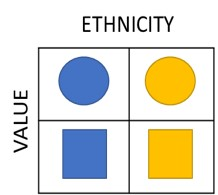
\includegraphics[width=0.7\linewidth]{model} 

}

\caption{Group-type of agents}\label{fig:model}
\end{figure}

In our model value orientation of agents is relevant for two reasons.
First, it determines an additional dimension of similarity which is
independent of ethnicity: liberals can recognize as similar
value-oriented also liberals of the other ethnic group, so as to
recognize of different value orientation conservatives of both ethnic
groups\footnote{Equally, also conservatives recognize similar value-oriented conservatives of both ethnic groups}.
Additionally, value orientation matters in defining the strength of
ethnic or value similarity in the relocation decision of agents. In
\cite{paolillo2018} agents randomly relocated to an empty node according
to a threshold function, based on ethnic composition for
ethnicity-oriented agents and value composition for value-oriented
agents. We substitute this behavior with a binary random utility
discrete choice model. At each time step, a random agent selects a
random empty node and compares its neighborhood composition to that of
its current node. By neighborhood of the agent we refer to the Moore
neighborhood of radius 1 of the agent selected; similarly, the
alternative neighborhood is the Moore neighborhood of radius 1 of an
empty cell. We substitute the threshold function in \cite{paolillo2018}
with a continuous linear function for both ethnic and value neighborhood
composition:

\begin{equation}
   U^e_j = \frac{x^e_j}{X_j}\quad\text{   ;    }\quad  U^v_j = \frac{x^v_j}{X_j}
\end{equation}

where:

\par

\(U^e_j\): ethnic utility of neighborhood \textit{j}

\par

\(x^e_j\): number of agents in neighborhood \textit{j} with same
ethnicity

\par

\(X_j\): total number agents in neighborhood \textit{j}

\par

\(U^v_j\): value utility of neighborhood \textit{j}

\par

\(x^v_j\): number of agents in neighborhood \textit{j} with same value

\par

\(X_j\): total number agents in neighborhood \textit{j}

\par

Both utilities can range {[}0,1{]}. Utility of a neighborhood is set to
0 if \(X_j = 0\), i.e.~not agents are in the neighborhood. The
probability for an agent to choose the alternative neighborhood over the
current one is modeled with a logistic function as:

\begin{equation}
    P_{al} = \frac{exp(\beta_e U^e_{al} + \beta_v U^v_{al})}{1 + exp((\beta_e U^e_{cr} + \beta_v U^v_{cr}) - (\beta_e U^e_{al} + \beta_v U^v_{al}))}
    \label{eq:lgst}
\end{equation}

where:

\par

\(\beta_e\): weight for ethnic preference

\par

\(\beta_v\): weight for value preference

\par

\(U^e_{al}\): ethnic utility of alternative neighborhood

\par

\(U^e_{cr}\): ethnic utility of current neighborhood

\par

\(U^v_{al}\): value utility of alternative neighborhood

\par

\(U^v_{cr}\): value utility of current neighborhood

\par

The higher \(\beta_e\) or \(\beta_v\), the higher the option with higher
ethnic or value utility is likely to be selected, the lower \(\beta_e\)
or \(\beta_v\), the higher the chance that selection is random for that
dimension. With both \(\beta_e = 0\) and \(\beta_v = 0\), the choice is
totally random and \(P_{al} = P_{cr} = 0.5\). This formula is a
transformation of Eq: \ref{eq:cndtnl} for a binary choice with
probability to relocate to alternative
neighborhood\footnote{The equivalence between logistic function  and conditional logit for two options is valid since the difference between random terms that are assumed to have a Gumbel distributions has a logistic distribution. The logistic function in Eq: \ref{eq:lgst} is transformation of Eq: \ref{eq:cndtnl} written as $P_{al} = \frac{exp(U_{al})}{exp(U_{al}-U_{cr})}$, resulting from division of numerator and denominator by numerator $exp(U_{al})$, with $exp(U_{cr})/exp(U_{al}) = exp(U_{cr}) - exp(U_{al})$ (see \cite[p.39]{train2009discrete} for detaills)}.
Probability computed is compared to a random number ranging between 0
and 1. If probability is higher than random number, then the agent moves
to the alternative neighborhood, leaving its cell empty. So, the
logistic function serves as a simplified version of the roulette wheel
selection
\footnote{see \cite{bruch2012methodological} for an example of roulette wheel selection}.

We opted for a binary choice to ease computational power required. As
tested, due to iterations of the model results would not change with
selection between more options. We opted for a continuous linear
function because default assumption in utility maximization and
sensitive to changes in neighborhood compositions, which is strategic to
our aim \citep{van2009neighborhood}. Moreover, it lets behavior of
agents differ only for parameters of determinism \(\beta_e\) and
\(\beta_v\), so to allow us to disentangle the effect of either ethnic
or value similarity preferences on emerging segregation.
{\textcolor{red}{Rocco: next paragraph: I mean that potentially one can span the parameters so to have ethnic liberal > ethnic conservative. We impose preferences as I describe because of theoretical consistency with our research goal}}
We vary \(\beta_e\) and \(\beta_v\) depending on the value orientation
of agents and in our experiments impose differences in heterogeneous
preferences between the two types of agents. Liberal agents, considered
as more prone to ethnic tolerance, hold higher value preferences: weight
for ethnic similarity cannot exceed their weight for value similarity
(\(\beta^{\circ}_v \geq \beta^{\circ}_e\)). Conservative agents hold
higher ethnic preferences: weight for value similarity cannot exceed
their weight for ethnic similarity
(\(\beta^{\Box}_e \geq \beta^{\Box}_v\)). Moreover, the heterogeneity
between conservative and liberal agents exists so that ethnic
preferences of liberals do not exceed those of conservatives
(\(\beta^{\Box}_e \geq \beta^{\circ}_e\)), and value preferences of
conservatives do not exceed those of liberals
(\(\beta^{\circ}_v \geq \beta^{\Box}_v\)).

As outcome of the model, we report the index of exposure for both ethnic
and value segregation of agents who have at least one neighbor. This is
the classic measure of segregation in Schelling and is equivalent to the
fraction of agents of same ethnicity or value orientation in the
neighborhood, indifferent to the actual number of neighbors.
Nevertheless, we consider this a best fir to our interest in hybrid
segregation scenarios. Since the measure is collected for all agents who
have at least one neighbor, an index equal 0 means assimilation of the
agent for that dimension, i.e.~exposed only to agents of different
ethnicity or value orientation. An index equal to 0.5 means that the
agent is perfectly integrated for that dimension, being exposed to
agents of different ethnicity or value orientation. An index equal 1
means total segregation, i.e.~exposure only to similar agents for that
dimension. Thus, the 2 indexes can be easily compared to visualize if
agents are assimilated, integrated or segregated for one dimension and
differently for the other.

\begin{table}[H]

\begin{tabular}{lll}
 \hline
\textbf{Agent definition}  & \textbf{Range}    \\ 
 \hline
 Ethnicity  (\textit{color})         & Blue (majority), Orange (minority)  \\
 Value orientation (\textit{shape}) & Square (conservative), Circle (liberal) \\
 Determinism ethnic utility ($\beta_e$) & $[0,\inf)$ 
 $\beta^{\Box}_e \geq \beta^{\Box}_v$
 $\quad\text{   ;    }\quad \beta^{\Box}_e \geq \beta^{\circ}_e$
 \\
 Determinism value utility ($\beta_v$) & $[0,\inf)$ $\beta^{\circ}_v \geq \beta^{\circ}_e$
 $\quad\text{   ;    }\quad \beta^{\circ}_v \geq \beta^{\Box}_v$\\
 \hline
\textbf{Global Parameters}  & \textbf{Range} \\ 
\hline 
 Population density      & $[0,0.99]$ \\
 Ethnic ratio majority/minority &  $[0,1]$ \\
 Value ratio conservative/liberal majority & $[0,1]$ \\
 Value ratio conservative/liberal minority  & $[0,1]$ \\
 \hline
 \textbf{Output measure}  & \textbf{Range} \\ 
\hline 
 Ethnic neighborhood exposure      & $[0,1]$ \\
 Value neighborhood exposure       & $[0,1]$ \\
 \hline
\end{tabular}
 \caption{Model parameters} 
 \label{tab:parameters}
\end{table}

\hypertarget{results}{%
\section{Results}\label{results}}

\hypertarget{baseline-conditions}{%
\subsection{Baseline Conditions}\label{baseline-conditions}}

We run our simulations for 1000 discrete time steps and run each
condition 20 times. We collected data for the last time step as
interested in the emerged equilibria resulting from relocation
preferences, population composition and degree of determinism.

In this first section, we report results for symmetric conditions so to
understand the key mechanisms of the model. At initialization, each
agent has \(50\%\) probability to be assigned to either majority or
minority ethnic group (equal ethnic size) and within each ethnic group,
\(50\%\) probability to be assigned to either conservative or liberal
value orientation. In short, each group-type represents \(25\%\) of the
population. Density of the grid inhabited is kept at \(70\%\) with
initial random distribution. Fig. \ref{fig:model_space} shows the
parameter space we explore in this baseline scenario and the figures
associated
{\textcolor{red}{Rocco: figures-experiment match to be updated in the end}}.
As measure of segregation, for both ethnic and value similarity, we
compute an index of exposure in the Moore neighborhood of agents who
have at least one neighbor. The index reports on average the fraction of
other agents of same ethnicity or same value orientation in the local
neighborhood of each agent. It ranges between \(0\), i.e.~exposure to
out-groups to \(1\), i.e.~full segregation, with \(0.5\) equal to
integration between the two groups. We report the index for ethnic
exposure (\(E_i\)) and value exposure (\(V_i\)) for each group-type:

\begin{equation}
   E_i = \frac{x^e_i}{X_i}\quad\text{   ;    }\quad  V_i = \frac{x^v_i}{X_i}
\end{equation}

where:\textbackslash{} \(x^v_i\): number of other co-value agents in the
Moore neighborhood of agent \textit{i}

\par

\(x^e_i\): number of other co-ethnic agents in the Moore neighborhood of
agent \text{i}

\par

\(X_i\): total number agents in neighborhood of agent \textit{i}

\par
\par

We report additionally the average density of the neighborhood agents
form, calculated as the fraction of inhabited grid cells in the Moore
neighborhood of agents. We are interested in density as indicator of
clustering of agents and how it relates to segregation patterns.

\begin{figure}[h]

{\centering 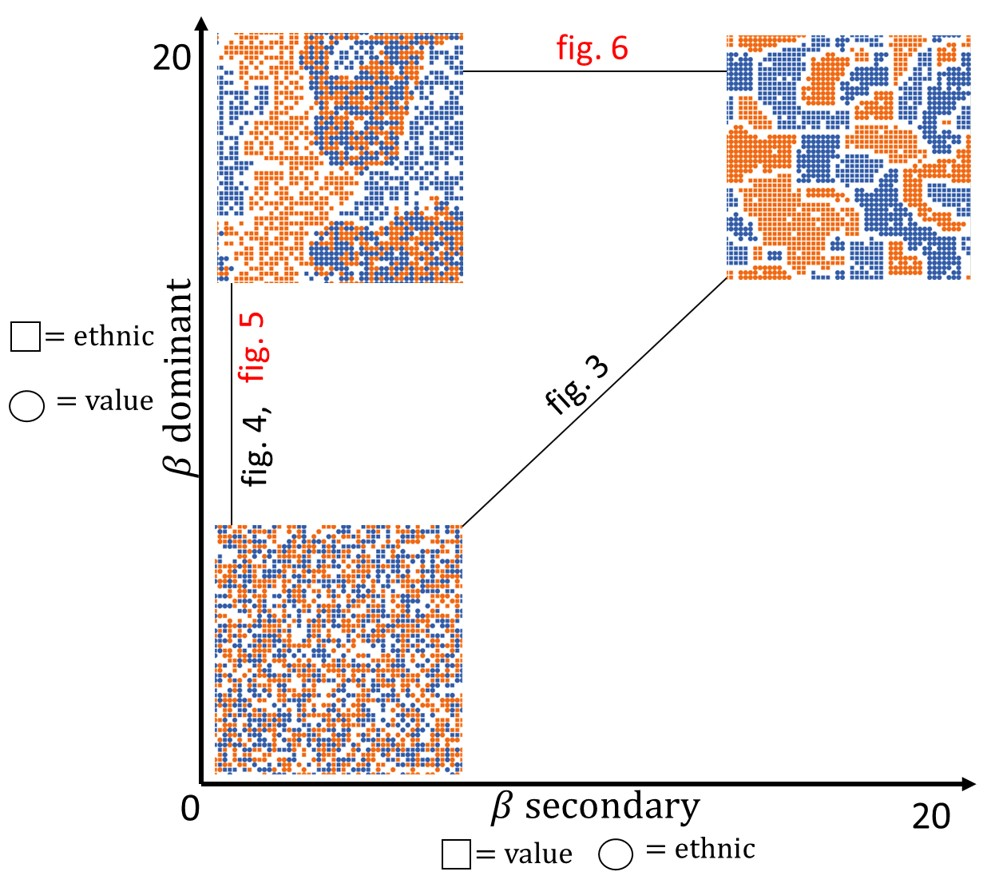
\includegraphics[width=0.7\linewidth]{model_space} 

}

\caption{Preference model space parameter and figure associated. Figure reference label: black color means liberals and conservatives hold same level of ß parameter (though with different definition of similarity). Red color means they hold different level of either dominant or secondary preference.Match figure-label to check/change in the end}\label{fig:model_space}
\end{figure}

Fig. \ref{fig:bsl} represents the baseline condition we compare results
to. Agents hold same preference for both ethnic and value segregation,
i.e.~they want to live close to agents of the same group-type. On the
x-axis, agents of both value-orientation increase their determinism
(parameter \(\beta\)). The graph shows how ethnic and value segregation
follow the same curve. Segregation increases monotonically from
\(\beta = 0\) until \(\beta = 7\) where full segregation is reached.
Density of neighborhoods remains basically unaltered from initial random
distribution, though slight increase when full segregation emerges at
\(\beta = 7\). Results mean that the size of neighborhoods of agents is
unaffected by increase of determinism, while their composition changes.

\begin{figure}[H]

{\centering 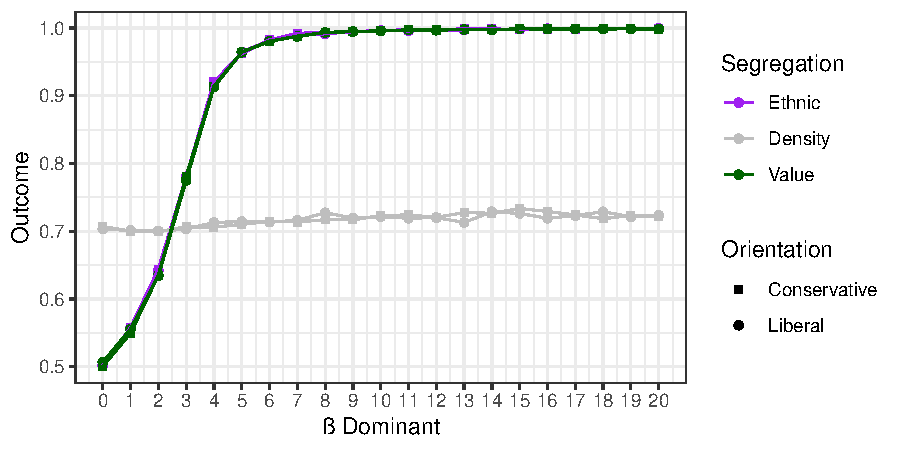
\includegraphics[width=0.8\linewidth]{ev_rum_files/figure-latex/bsl-1} 

}

\caption{Baseline condition. Each group-type represents 25\% of population. ß dominant = ß secondary}\label{fig:bsl}
\end{figure}

In Fig. \ref{fig:bsl_dom}, we investigate the scenario where agents hold
only to their dominant preference. Differently from previous condition
where agents would prefer someone with own identical characteristics,
liberals would relocate close to other liberals of different ethnic
group, as well as conserative try to maximize on ethnic utility with
liberal co-ethnics. This is ideal to investigate effects of different
preferences. For each type of agent, \(\beta\ dominant\) increases on
the x-axis, while \(\beta\ secondary = 0\) The figure shows how liberal
agents remain ethnically integrated, which is coherent with their random
relocation for ethnic dimension of neighborhoods (secondary preference
\(\beta_e = 0\)) with almost full value segregation. For conservative
agents, ethnic segregation is higher than value segregation of their
value counterpart, with full ethnic segregation reached with highest
determinism. What is unexpected is that also value segregation emerges
with increase in determinism, while their value preference is imposed to
\(\beta_v = 0\).

\begin{figure}[H]

{\centering 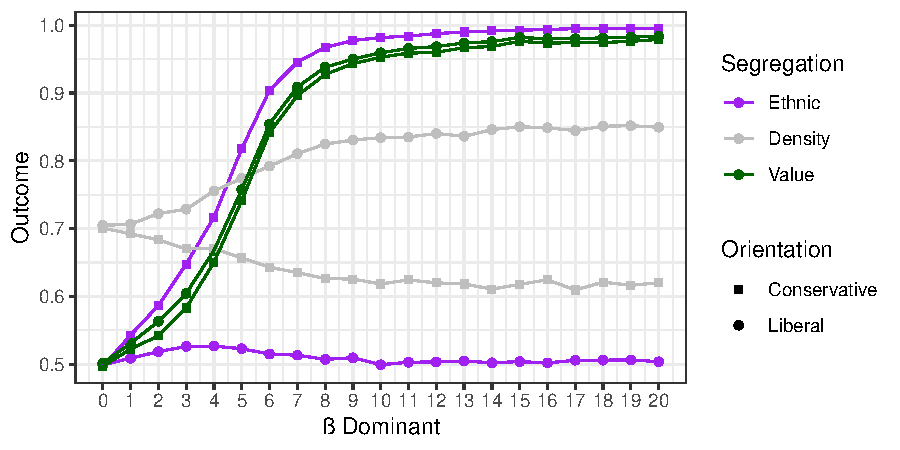
\includegraphics[width=0.8\linewidth]{ev_rum_files/figure-latex/bsl_dom-1} 

}

\caption{Baseline condition, ß dominant preference (ethnic for conservative, value for liberals on the x-axis), ß secondary preference (value conservative, ethnic liberal) equal to 0}\label{fig:bsl_dom}
\end{figure}

Value segregation of conservatives occurs as a by-product effect of
value preference of liberals, due to the different definition of
similarity in spatial sorting. Due to symmetric condition, both
conservatives and liberals could potentially consider half of the
population as similar to maximize homophily preferences (population
equally split into two ethnic groups and two value orientations).
However, though conservatives would relocate close to liberal
co-ethnics, they would be rejected by the latter who would prefer a
neighborhood with other liberals, while both conservatives and liberals
of the other ethnic group would be rejected based on the own ethnic
preference. In short, conservatives of each ethnic group can only count
on other conservatives of their own ethnicity to form stable
neighborhood, equal to \(25\%\) of the population. On the other side,
liberals would relocate close to co-values of both their own and the
other ethnic group, so to count on \(50\%\) of the population to
maximize value utility, i.e.~the double of percentage available to
conservatives. The result is that liberals form denser neighborhoods
compared to conservatives, because they have more similar agents to
relocate close to. Looking at Fig. \ref{fig:bsl_dom}, as determinism
increases, density of neighborhood of liberals increases from the
initial distribution, while conservatives' falls below it. By-product
occurs because liberals, avoiding conservatives of both ethnic groups
and forming denser neighborhood, reduces the space available on the grid
where conservatives of both groups can relocate, so to break also their
neighborhoods. Additionally, conservatives would sort with conservatives
of their own ethnic group.

\begin{figure}[H]

{\centering 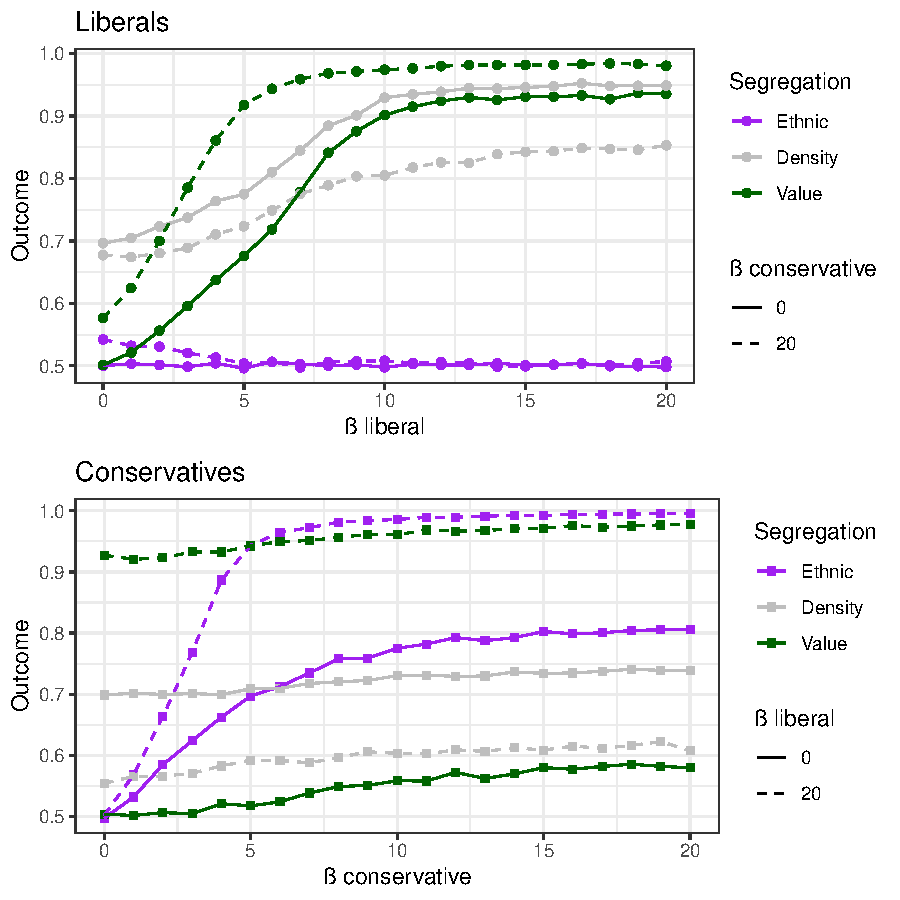
\includegraphics[width=0.7\linewidth]{ev_rum_files/figure-latex/bsl_fct-1} 

}

\caption{Baseline condition, for each value-orientation type, how its patterns are influenced by determinism of the other group. Secondary preference in each condition is equal to 0. Top panel liberals: ß value liberals on x-axis, linetype: ß ethnic conservative equal 0 or 20; Bottom panel: ß ethnic conservative on x-axis, linetype: ß value liberal.}\label{fig:bsl_fct}
\end{figure}

Fig. \ref{fig:bsl_fct} clarifies how the segregation patterns of each
group-type liberals and conservative depends on their dominant
preference or it is influenced by preferences of other group-type as
by-product. On top panel, results for liberals are reported. On x-axis,
liberals increase determinism ß value in their relocations, linetype
shows the conditions due to behavior of conservatives: total random
relocation ß = 0, or extreme determinism ß = 20. The picture shows how
the density of neighborhoods liberals form increases with increase of ß
value, though i shows lower levels when conservatives hold max ß ethnic,
compared to Fig. \ref{fig:bsl_dom}. While ethnic integration is
unaltered by ethnic preference of conservatives, as no difference is
evident. On the contrary, value segreation seems higher when
conservative cluster together until ß conservative = 20. Likely with ß =
0 they would randomnly relocate into neighborhoods of liberals, thus to
decrease their value utility. The difference is higher for lower
determinism area. The bottom panel repeats for conservative agents
influenced by behavior of liberals. With ß liberal = 0, a slight
increase emerges for higher determinism of conservatives, i.e.~they can
cluster only with other conservatives of their ethnic group, and taking
adavantage of liberal co-ethnics who randomly relocate. With ß value
liberals = 20, the by-product is evident and strong: value segregation
basically does not increase for all levels of ß ethnic conservative and
remains high. In short, the value segregation of conservatives is very
minimally due to clustering due to ethnic preference. Neighborhood
density remains equal to initial distribution with ß value liberal = 0,
meaning conservatives do not form denser neighborhoods as liberals,
which can be related to have lower ethnic segregation compared to value
segregation of liberals when conservative hold ß ethnic = 0.
Neighborhood density decreases and remains constant when ß value
liberals = 20, being their space in the grid limited by neighborhoods
formed by liberals and forming conservatives less dense neighborhoods.
However, though neighborhoods are less dense, the ethnic exposure for
conservatives reaches full segregation.

\begin{figure}[H]

{\centering 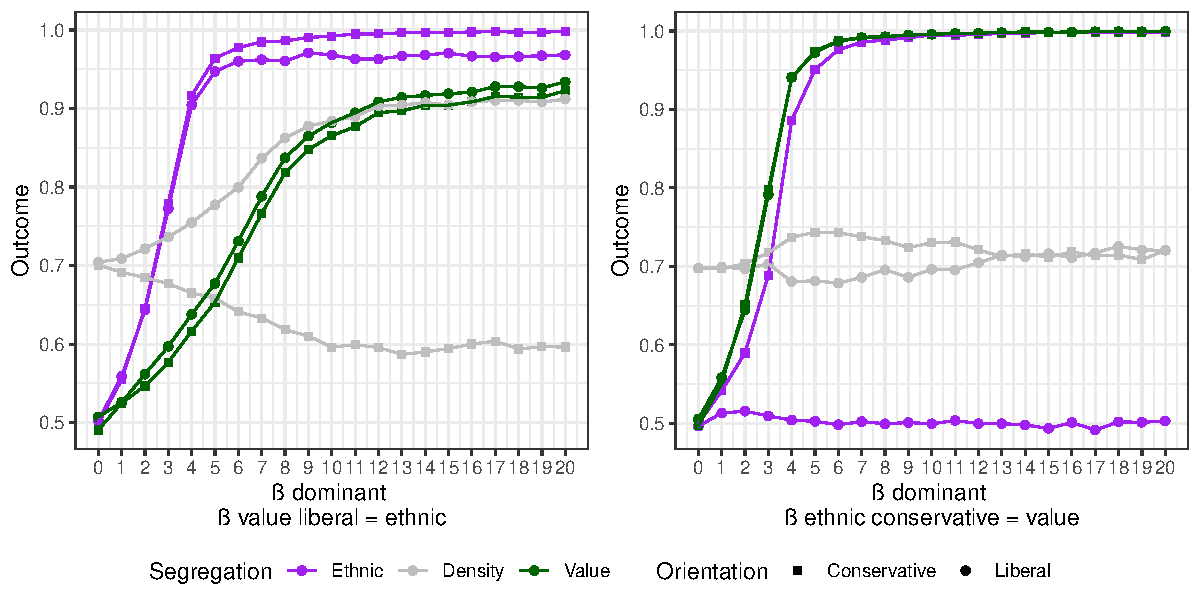
\includegraphics[width=1\linewidth]{ev_rum_files/figure-latex/bsl_sec-1} 

}

\caption{Baseline condition, Effect of agents holding ß dominant = ß secondary, comparison of different preferences. On the x-axis, increase ß dominant for all agent. Left panel: liberals hold value preference (dominant) equal to ethnic preference (secondary); left panel: conservatives subscribe only to ethnic preference. Right panel: liberals hold ethnic preference (dominant) equal to value preference (secondary)}\label{fig:bsl_sec}
\end{figure}

Fig. \ref{fig:bsl_sec} repeats Fig. \ref{fig:bsl_dom} but with the
difference that conservatives and liberals hold secondary preference
equal to dominant preference. The aim is to compare with Fig.
\ref{fig:bsl} and Fig. \ref{fig:bsl_dom}: how they would change if also
secondary preferences are taken into consideration, and allow to observe
how degree of determinism influences the process. This was the best
solution to include all into feasible picture so far. Lower value
segregation of conservatives as by-product, as they are more accepted by
liberals and shift in density neighborhood of conservatives. To think
about.

Heatmap in Fig. \ref{fig:htmp} shows instead other combinations that
would not be included in Fig. \ref{fig:bsl_sec}: e.g.~fix one level of
determinism ß value and increase ß ethnic of liberals. However, all
agents hold same degree of determinism, which obscures whether agents
cluster because of increase in secondary preference, or because of
by-product e.g.~for areas of high determinism.

\begin{figure}[H]

{\centering 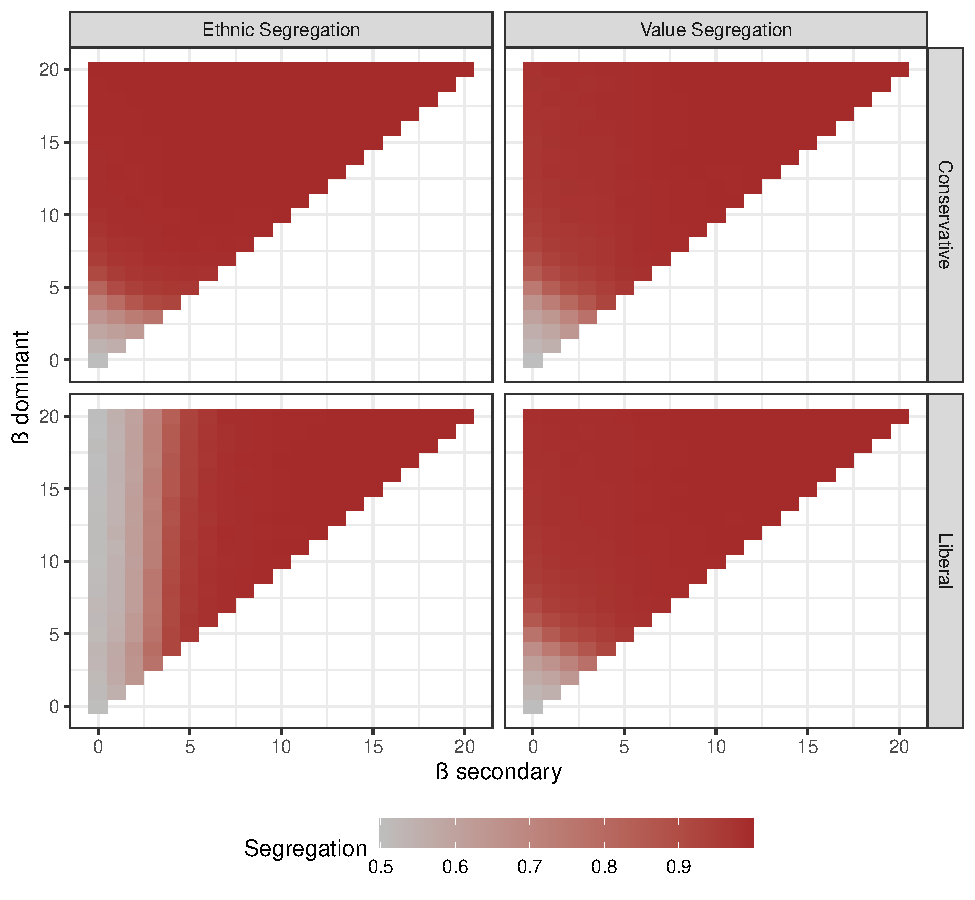
\includegraphics{ev_rum_files/figure-latex/htmp-1} 

}

\caption{Basic condition. Heatmap generated by ß dominant preference (ethnic for conservative, value for liberals) and secondary preference (value for conservatives, ethnic for liberals). Liberals and conservatives hold same level of ß dominant and ß secondary in each condition (global parameter)}\label{fig:htmp}
\end{figure}

\hypertarget{asymmetric-conditions}{%
\section{Asymmetric Conditions}\label{asymmetric-conditions}}

The main focus is on scenario with secondary ß = 0 (Fig:
\ref{fig:bsl_dom}), since it shows most interesting results as
by-product. In this section we want to show how segregation scenarios
that in the previous section depended on different homophily preferences
can vary if agents hold similar preferences but distribution in
population composition differ (e.g.~majority influences more than
minority, ceteris paribus). The main focus for simplicity is on
preference of liberals majority vs liberals minority, since they enact
mechanisms as by-product and represent new introduction to Schelling's
model (see figures in details). So also for increase of secondary ß For
simplicity of visualization and to focus on preferences of agents,
\(80\%\) ethnic ratio is considered in the experiments. For value
orientation, as in the asymmetric condition, each ethnic group equally
split into liberals and conservatives (i.e.~50\% of population is
liberal, and 50\% conservative, but more chance of both conservative and
liberal to belong to ethnic majority). Fig:\ref{fig:dislib_fig} and Fig:
\ref{fig:dislib_ethnic} are to show how results would change in the full
conditions due to joint distribution ethnic ratio and distribution of
liberals which affect population composition. In particular distribution
of liberals is of interest because it allows to break the ethnic
unbalance between liberal majority and minority, how conservatives of
both groups react to increase of liberals in the population, and how
effective change in the minority population would be, if an ethnic
critical mass is not reached. Basically in all conditions majority
remains split 50\% into liberals and conservatives, but both changes in
minority population are more interesting to relate to change into the
integration/segregation continuum.

In ethnic asymmetric conditions, we use the spatial relocation index to
measure whether segregation occurs from initial random distribution.
Local exposure can be computed from it, but it is not intuitive to
reader in my view. In the tables in appendix, the reader can see for
each condition what local exposure matches spatial clustering of agents.

\begin{equation}
    E^c_i = \frac{(\sfrac{x^e_i}{X_i})}{(\sfrac{N^e_i}{N})}  \quad\text{        ;          }\quad  V^c_i = \frac{(\sfrac{x^v_i}{X_i})}{(\sfrac{N^v_i}{N})} 
\end{equation}

where:

\par

\(x^e_i\): number of co-ethnics neighbors of agent \textit{i}

\par

\(x^v_i\): number of co-values neighbors of agent \textit{i}

\par

\(X_i\): number of neighbors of agent \textit{i}

\par

\(N^e_i\): number of agents in the population with same ethnicity of
agent \textit{i}

\par

\(N^v_i\): number of agents in the population with same value of agent
\textit{i}

\par

\(N\): total number of agents in the population

\par

\par

Fig: \ref{fig:asm_dom} wants to inform the reader of what is the direct
effect of different ethnic ratio and how spatial clustering relates to
local exposure. It replicates Fig: \ref{fig:bsl_dom} comparing the
condition of ethnic equal size (\(50 \%\)) vs majority/minority
condition used in this section (\(80\%\)). Results show given the same
ethnic preference, conservative minority have higher need to cluster to
satisfy ethnic utility, resulting in higher spatial clustering, 5 times
the initial random distribution, with increase of local ethnic exposure
to 1 (0.2*5). While for conservative majority, similar full ethnic
exposure is reached with lower spatial clustering, since there is more
chance to find co-ethnics in the population. For both liberals majority
and liberals minority full value segregation is reached with value
spatial clustering equal 2, i.e.~full local value exposure equal 1.
Ethnic segregation does not occur in terms of spatial clustering from
initial distribution for both liberals majority and liberals minority,
meaning higher ethnic exposure of liberals majority to 80\% and ethnic
assimilation for liberals minority 20\%

\begin{figure}[H]

{\centering 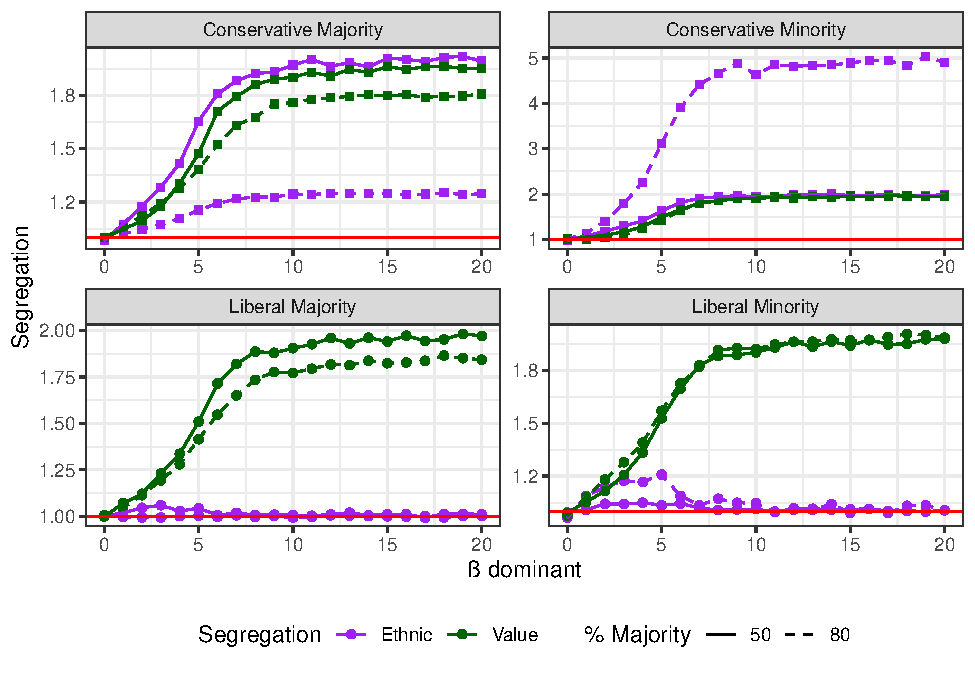
\includegraphics{ev_rum_files/figure-latex/asm_dom-1} 

}

\caption{Baseline ethnic asymmetric condition. Each panel reports the segregation pattern of each group-type (ethnicityXvalue). X-axis: ß dominant (ethnic for conservative, value for liberals), Y-axis: dislocation index. Agents hold only dominant preference: ß secondary = 0. Linetype: comparison equal ethnic size (50 \%) vs majority/minority condition (80\%).}\label{fig:asm_dom}
\end{figure}

\begin{figure}[H]

{\centering 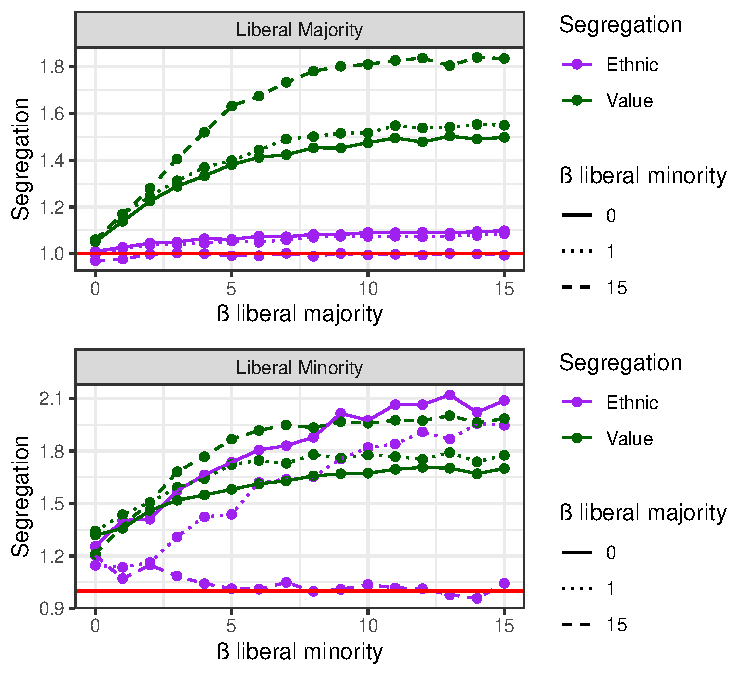
\includegraphics[width=1\linewidth]{ev_rum_files/figure-latex/asm_lib_lib-1} 

}

\caption{Ethnic asymmetric: effect dominant preference (ß value) liberals minority over liberals majority (top panel) vs effect liberals majority over liberals minority (bottom panel). For each panel, on x-axis increase ß value preference of group-type, linetype: ß value preference of out-group counterpart. Conservative agents hold to dominant ethnic preference ß = 15. Secondary preference for both conservative and liberals = 0}\label{fig:asm_lib_lib}
\end{figure}

Fig: \ref{fig:asm_lib_lib} first explores how liberals majority and
minority influence each other, basically to explore whether ethnic
integration at local exposure can be reached as due to different value
preferences of either group, or ethnic assimilation of minority and
value segregation of both in Fig: \ref{fig:asm_dom} would be affected.
Each panel shows results of liberals majority (top) and liberals
minority (bottom). For each graph, results show changes due to ethnic
counterpart having no preference at all (ß = 0), low value determinism
(ß = 1) or high value determinism (ß = 15). In all conditions,
conservatives of both ethnic groups hold ß ethnic = 15, so to have
stable ethnic segregation pattern from their behavior.

Liberals majority are lower affected by value preference of liberals
minority for what concerns ethnic segregation. Basically if the other
group doesn't care about value homophily, the agents can relocate only
close to liberal co-ethnics. For liberals majority not much change in
spatial clustering occurs because of majority condition, while for
liberal minority the same condition leads from ethnic assimilation to
ethnic segregation, though ethnic preference is not involved. Even a
small amount of determinism of liberals majority is enough to increase
value segregation of liberals minority (see bttom panel with ß liberal
minority equal 0). However, in top panel, higher value segregation is
reached by liberals majority for higher determinism if liberal minority
hold high ß value = 15

I included ß = 0 of ethnic counterpart as theoretical baseline: what
happens if there no preference at all in the ethnic counterpart.
Methodologically is correct to include in my view, though difference
with ß=1 is not that stricking. We could think of cutting off if the
figure is too complicated.

\begin{figure}[H]

{\centering 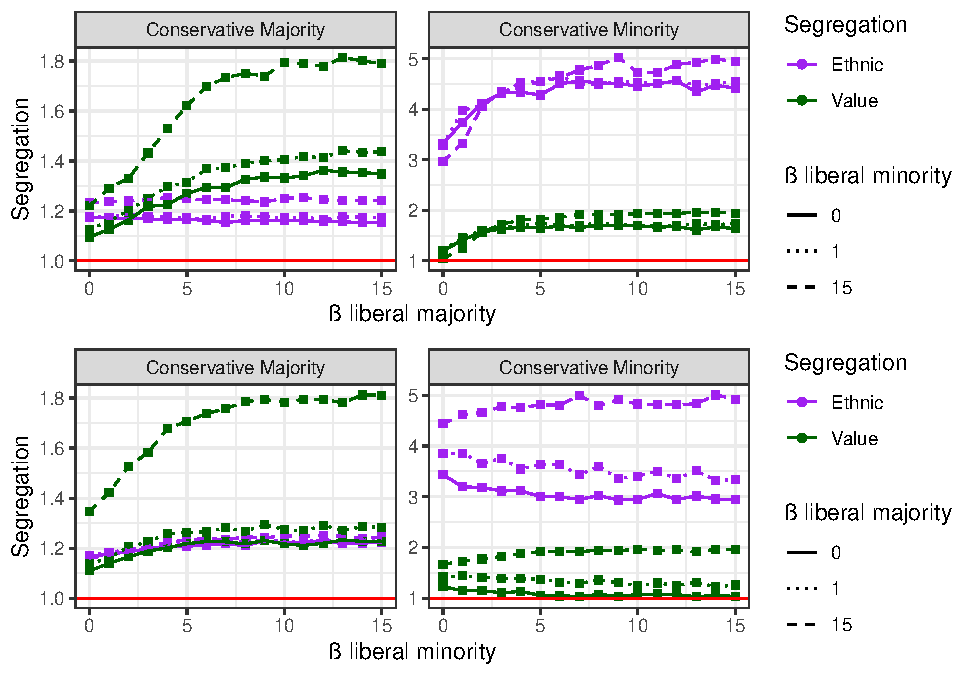
\includegraphics[width=1\linewidth]{ev_rum_files/figure-latex/asm_lib_con-1} 

}

\caption{Ethnic asymmetric: effect of ß value liberals majority or liberals minority over conservatives majority and conservatives minority. Each panel reports pattens of conservative majority (left) or conservative minority (right). Top panel: effect of ß value liberals majority (on x-axis), linetype: changes due to different levels of ß value liberal minority. Bottom panel: effect of ß value liberlas minority (on x-axis), linetype: changes due to different levels of ß value liberal majority. Conservative agents hold to dominant ethnic preference ß = 15. Secondary preference for both conservative and liberals = 0}\label{fig:asm_lib_con}
\end{figure}

Fig: \ref{fig:asm_lib_con} focuses on effect of liberals majority and
liberals minority over conservatives. The idea is to observe how the
effect of liberals can vary depending on the value preference of ethnic
counterpart, and how conservatives can differently being affected due to
ethnic asymmetry. Expected: liberals majority have more influence than
liberals minority, conservative majority are less affected than
conservative minority.

The picture shows influence of liberals majority on top panel, liberals
minority on bottom panel. If too complicated, we could split. Also here,
ß liberals ethnic counterpart as baseline, if too complex we could get
it off.

Value segregation of conservative majority show similar patterns whether
value of liberals minority is swept or liberals majority. Ethnic
segregation (spatial clustering) of conservative minority is already
high due to ethnic minority as Fig: \ref{fig:asm_dom} has shown, but it
increases as liberal majority increase ß value, as effect of rejection
and limiting their space of relocation. This can be considered a
by-product by ethnic asymmetry, compared to by-product by value in
symmetric condition. Looking at bottom panel, for lower ß liberal
majority, increase in ß liberal minority seems to slightly decrease
ethnic segregation of conservative minority. Likely liberals of both
ethnic groups form dense, value homogeneous neighborhoods with few
liberals majority who are not sensitive to conservatives because of
lower determinism, while liberals minority because value utility
maximization is preserved, since few conservative minority. So,
conservative minority can maximize ethnic utility at cost of living
close to few liberals of majority group, which decreases the spatial
clustering. As ß liberal majority = 15, increase in ß liberal minority
is associated with higher ethnic clustering of conservative minority as
in the top panel.

\begin{figure}[H]

{\centering 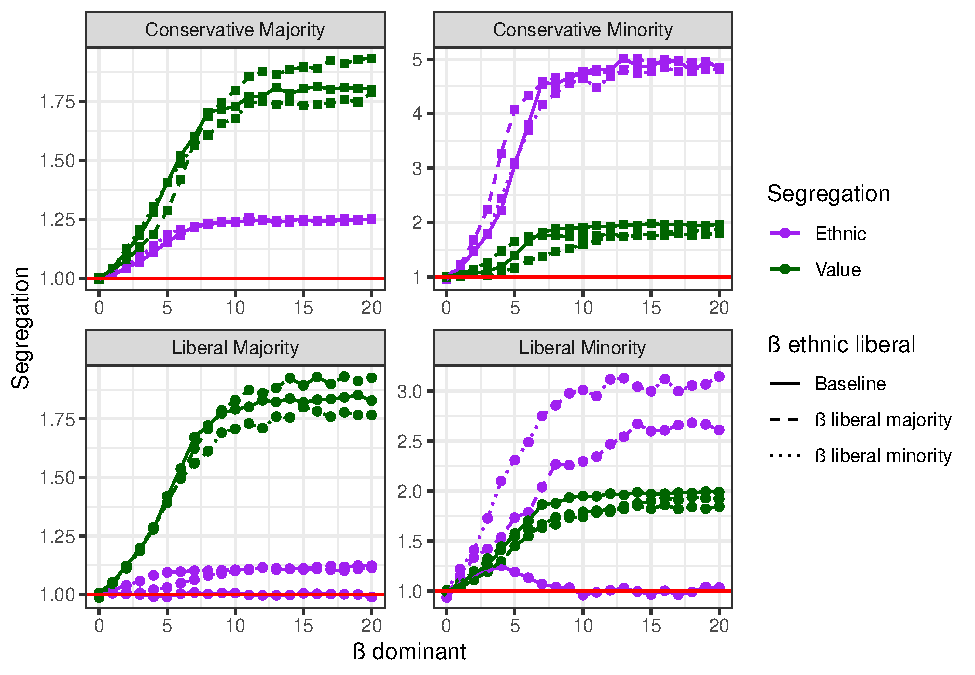
\includegraphics[width=1\linewidth]{ev_rum_files/figure-latex/et_lib-1} 

}

\caption{Ethnic asymmetric: effect of ß ethnic of liberals (secondary) equal to ß value liberals (dominant. x-axis: increase dominant preference for all agents (global parameter). Each panel reports segregation patterns of each group-type (ethnicXvalue). Linetype represents conditions compared: baseline: liberals of both ethnic groups hold  only to dominant preference (ß secondary = 0); ß liberal majority = liberals majority hold same ethnic and value preference (liberals minority hold only to value preference), ß liberal minority = liberals minorty hold same ethnic and value preference (liberals majority hold only to value preference)}\label{fig:et_lib}
\end{figure}

Finally, Fig: \ref{fig:et_lib} shows effect of liberals majority or
liberal minority holding both ethnic and value preference. Compared to
Fig: \ref{fig:bsl_sec}, we observe how ethnic asymmetry interacts with
degree of determinism. Each panel reports result for one group-type and
compares a baseline where agents only subscribe to ß dominant (ß
secondary = 0), to liberals majority subscribing also to ß ethnic or
liberals minority doing so.

Generally to interpret deeper. Liberals majority holding also ethnic
preference increases the value by-product for conservative majority for
high determinism compared to baseline, lower for higher randomness. For
conservative minority, liberals majority holding also ethnic preference
increases ethnic segregation compared to baseline for higher randomness
are, liberals minority holding also ethnic preference shows no
difference from baseline. Differences between conditions disappear for
high determinism. For value segregation of conservative minority, lower
value segregation as by-product occurs if liberals minority hold also
ethnic preference in higher randomness area, it increases for liberals
majority holding also ethnic preference. For higher determinism,
differences between liberals majority and liberals minority disappear,
with baseline showing (very slight) higher value.

For liberals majority, slight difference in value segregation occurs for
high determinism, with higher value segregation of liberals majority if
they hold also to ethnic preference, lower if liberals minority hold
also ethnic preference. Slightly decrease in ethnic segregation for
higher randomness if liberals majority hold also to ethnic preference.
For liberals minority differences are more evident: value segregation
decreases compared to baseline equally if liberals majority or liberals
minority increase hold also ethnic preference. If liberals majority hold
ethnic preference, ethnic segregation of liberals minority increases as
they increase ß value preference, since they can count only on liberals
co-ethnics to maximize value utility. If also minority were to hold
ethnic preference, ethnic segregation would be even higher, as direct
effect of their preference, decreasing value segregation because they
would accept more co-ethnic conservatives.

\begin{figure}[H]

{\centering 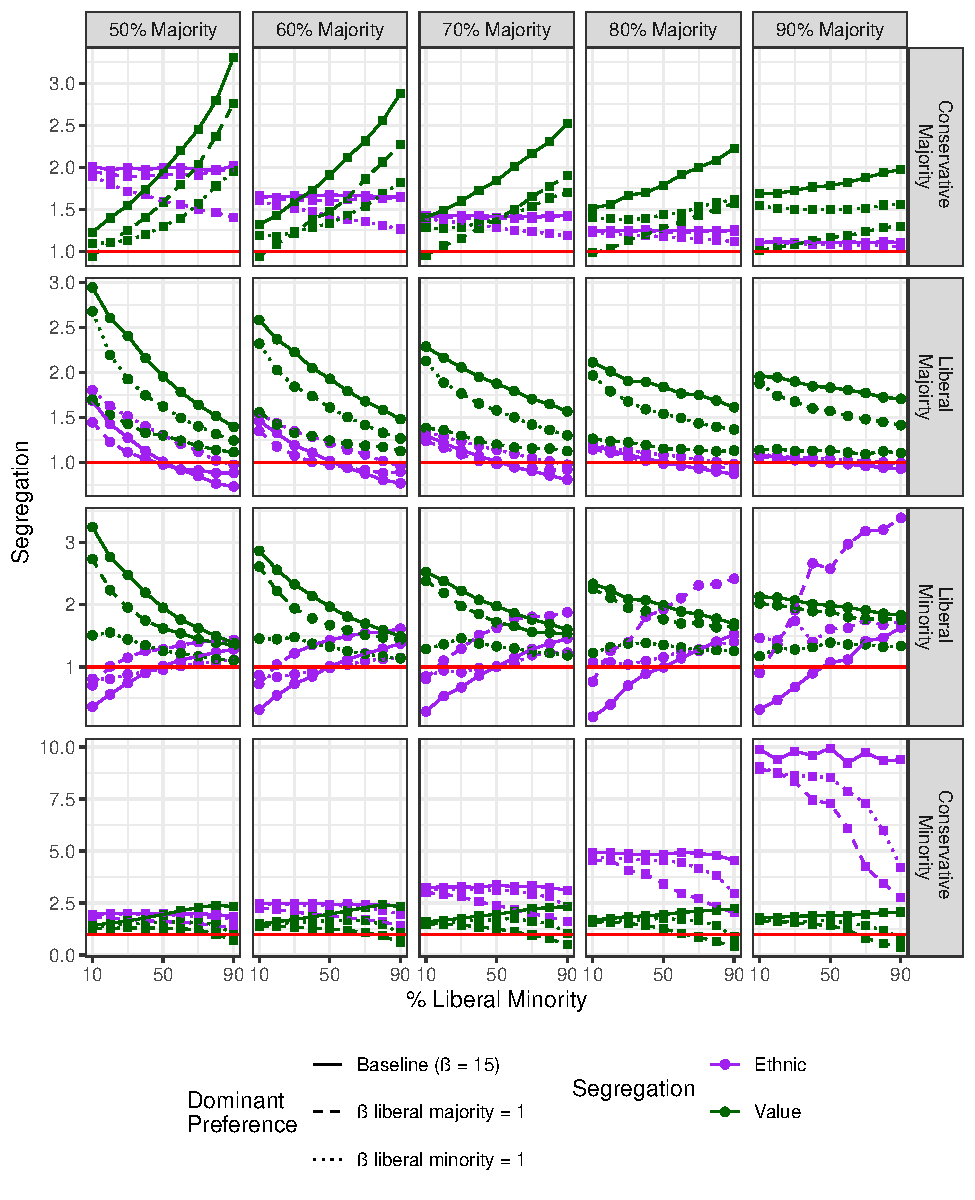
\includegraphics{ev_rum_files/figure-latex/dislib_fig-1} 

}

\caption{Comparison of lower determinism in liberals majority or liberals minority, effect of ethnic size and distribution of liberals. X-axis: pecentage of liberals of ethnic minority, column: ethnic ratio majority/minority. Each row reports the behavior of specific group-type. Linetype: conditions compared. Baseline: all agents hold dominant preference ß = 15,  secondary preference ß = 0; ß liberal majority = 1: liberals majority have minimum determinism (liberals minority hold to ß value = 15); ß liberal minority = 1: liberals minority have minimum determinism (liberals majority hold to ß value = 15). Conservatives of both ethnic groups hold to ß ethnic = 15 in all conditions}\label{fig:dislib_fig}
\end{figure}

Fig: \ref{fig:dislib_fig} compares baseline dominant ß = 15 to either
lower value determinis (ß = 1) of either liberals minority and liberals
majority, and highlights differences due to population composition due
to ethnic asymmetry and distribution of liberals.

I have to think about more. More interesting result is liberal majority
falling into ethnic assimilation because of value preference, provided a
critical mass is reached between ethnic ratio and distribution of
liberals. Even if liberals minority increases, but their ethnic group is
underrepresented, homophily based on value similarity will not make a
difference. I think there are insights for the majority-minority
paradigm and diverse societies here, with due limits. Anyway, I have to
think of for the specific conditions.

I include 90\% conclusion for completeness. However, this creates an
extreme condition where segregation/assimilation occurs mostly for
ethnic asymmetry, it is too unbalanced and value to extreme compared to
others. However, we can decide about later.

\begin{figure}[H]

{\centering 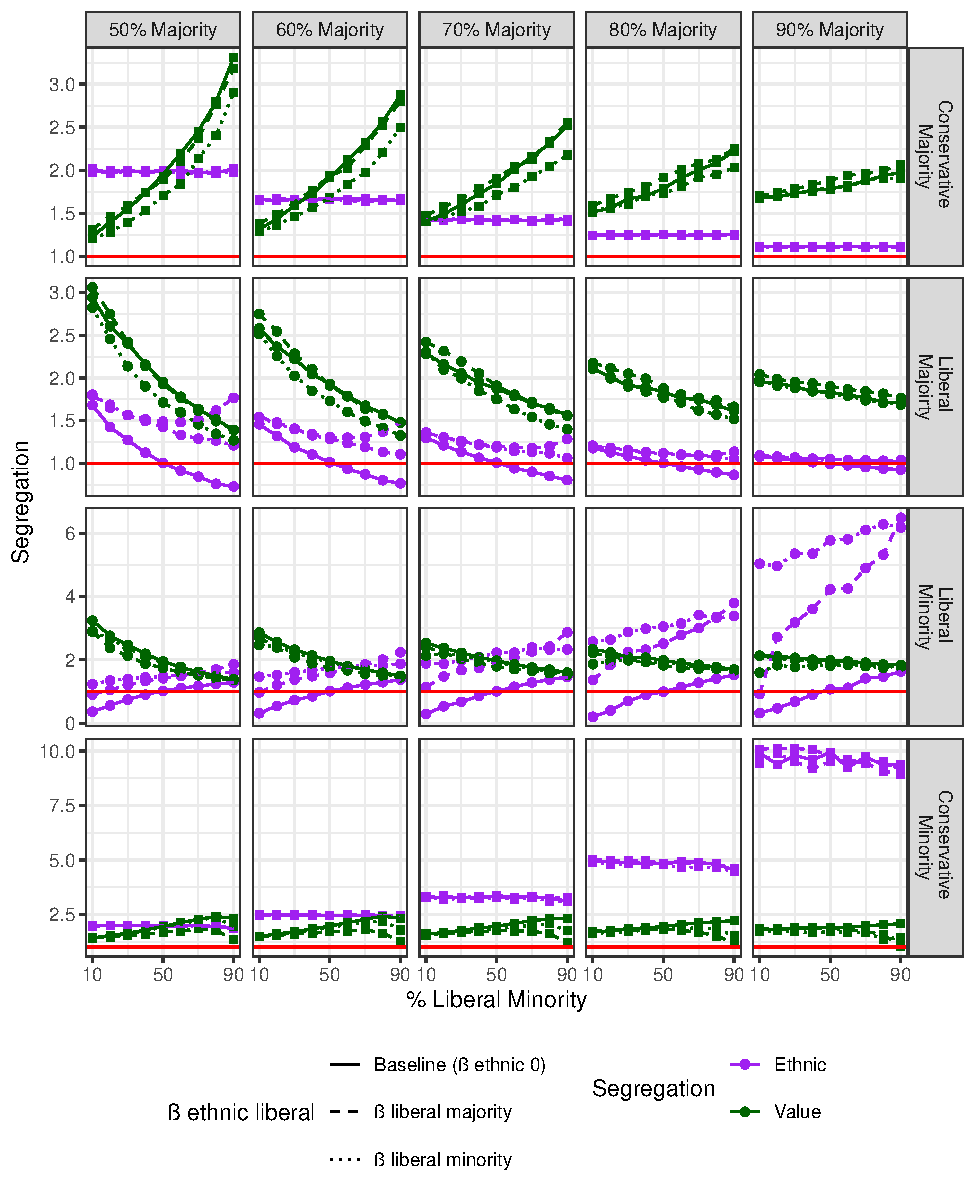
\includegraphics{ev_rum_files/figure-latex/dislib_ethnic-1} 

}

\caption{Comparison of liberals holding both ethnic and value preference, effect of ethnic size and distribution of liberals. Linetype: conditions compared. Conservatives of both ethnic groupd hold ß ethnic = 15 and ß secondary (value) = 0. Baseline: both liberals and  conservatives hold dominant preference ß = 15 and sercondary ß = 0; ß liberal majority = liberals majority hold both ethnic and value preference ß = 15 (liberals minority hold ß value = 15 and ß ethnic = 0); ß liberals minority = liberals minority hold both ethnic and value preference ß = 15 (liberals majority hold ß value = 15 and ß ethni = 0)}\label{fig:dislib_ethnic}
\end{figure}

Fig: \ref{fig:dislib_ethnic}, same as Fig: \ref{fig:dislib_fig} for
liberals holding also to ethnic preference, how segregation will differ
from baseline ß = 15 and for combination ethnic size and distribution of
liberals. Seems less changes, but it has to be thought about.

\hypertarget{discussion-and-conclusions-working-on}{%
\section{Discussion and Conclusions (working
on)}\label{discussion-and-conclusions-working-on}}

{\textcolor{red}{Rocco: more to the point: societies show lower ethnic segregation, increasing other dimensions (e.g. ses), and literature shows other characteristics matter $>$ acs2018 $>$ now discrete choice and other extension, in medias res; results similar to \cite{paolillo2018}}}

Schelling's model is often cited to describe how high levels of spatial
ethnic segregation can persist in society even if people hold slight
preference to live close to co-ethnics. However, the high complexity of
current society challenge some assumption of the model. In particular,
people belong to different categories, both within and between ethnic
groups, and literature suggesting ethnicity could be less relevant than
other categories to define similarity preferences in relocation choice.
In this paper we wanted to extend Schelling to these scenario. We built
on \cite{paolillo2018} extension of Schelling to the scenario of members
of the same ethnic group sharing common attributes with out-groups and
holding higher preference for either ethnic membership or secondary
characteristics. We extend the model to discrete choice random utility
models, testing on effect of different weights (level of randomness) of
agents and letting agents hold both ethnic and value preference. Our
results confirm some peculiarities of value similarity based on shared
attributes across ethnic membership despite our change to the decisional
process of agents. First, value similarity can induce a by-product
segregation of conservatives who do not care about secondary attributes.
Second, value similarity form denser neighborhoods due to inclusion of
co-values from both ethnic groups; neighborhoods become more resilient
to fluctuations in neighborhood composition. As already observed in
\cite{paolillo2018} the tendency is to form robust neighborhood value
homogeneous but ethnically integrated.

Most results are similar to \cite{paolillo2018} because a thereshold = 0
equals to randomness \(\beta = 0\) in terms of relocation decision of
agents and aggregated results. However, inclusion of randomness, along
with preference for both ethnic and value similarity, and senstivity to
different group size, show different highlights on the segregation
process.

Our results show who the definition of similarity based on shared
characteristics might be not sufficient to guarantee spatial integration
between groups. If people care about both ethnic and value similarity,
full segregation for both dimension would lead to division of society in
four group-types. However, lower determinism in the relocation choice
can decrease segregation. If liberals become more ethnically
conservatives, they would need higher preference to reach full ethnic
segregation, as long as conservatives not care about secondary
preference. On the contrary, value segregation of conservatives would
not increase if they were to increase value preference, as long as
liberals are enough to enact by-product value-segregation. This could
explain why segregation by ses seems stronger than ethnic segregation
{\textcolor{red}{Rocco: costs to be considered}} and ethnic homogeneous
neighborhoods are often also ses and educational homogeneous
{\textcolor{red}{Rocco: link to double segregation in Fossett, not because of affordability, but because of by-product of other classes wanting to segregate}}.
Sensitivity analysis shows the role of relative sizes. First, effects
due to majority are higher, this is evident from liberals majority who
can cause more changes in the model. Even if liberals minority could
cause the same mechanism, they don't reach a critical mass to do so.
Relative size show how same preference in terms of weights can have
different effect: for majority remaining in high ethnic exposure though
not spatially segregating, while for minority higher spatial clustering
emerges to satisfy even low preference. Segregation patterns of
liberals: even if liberals of two ethnic groups recognize each other as
similar, this would not translate into integrated neighborhoods because
of relative sizes. The result shows ethnic assimilation of liberals
minority separated from their co-ethnics with different secondary
attributes. Only if distribution of liberals increases to a certain
critical mass, the ethnic exposure of majority as effect of value
similarity would diminish We show how integration can emerge from the
condition where majority increase ethnic preference, through adaptation
between liberals and conservatives of minority group and the spatial
configurations formed.

{\textcolor{red}{Rocco: to compare with Schelling: how segregation is a stable results, when and why in our model integration can emerge}}

In Schelling, segregation as unstable condition results from all agents
holding the same threshold (hold same preference) within spatial
constraints and cascades that change neighborhood composition. In our
results, segregation would equally emerge if agents hold high
deterministic preference (higher \(\beta\)) for both dimensions.
Integration will persist if agents hold random behavior for either or
both dimensions, and the structural conditions of ethnic sizes and value
distribution

Limits: a mix of linear combinations, all can be predicted, once the
model is understood.

Next steps: to overcome tendency to segregation, a first step is to
change the shape of utility function, along with the two-dimensional
homophily behavior.
{\textcolor{red}{Rocco: This links to the literature showing how segregation emerges also for integrationist preferences (Zhang, Van Rijt etc.) third paper of the dissertation I am working on}}

\hypertarget{annex-robustness-analysis}{%
\section{Annex: Robustness Analysis}\label{annex-robustness-analysis}}

\begin{table}[H]

\caption{\label{tab:bsl_t}$\beta$ dominant = liberal}
\centering
\resizebox{\linewidth}{!}{
\begin{tabular}[t]{r|r|r|r|r|r|r|r|r|r|r|r|r}
\hline
\multicolumn{1}{c|}{ } & \multicolumn{6}{c|}{Conservatives} & \multicolumn{6}{c}{Liberals} \\
\cline{2-7} \cline{8-13}
\multicolumn{1}{c|}{ } & \multicolumn{2}{c|}{Ethnic} & \multicolumn{2}{c|}{Value} & \multicolumn{2}{c|}{Density} & \multicolumn{2}{c|}{Ethnic} & \multicolumn{2}{c|}{Value} & \multicolumn{2}{c}{Density} \\
\cline{2-3} \cline{4-5} \cline{6-7} \cline{8-9} \cline{10-11} \cline{12-13}
Dominant & Mean & SD & Mean & SD & Mean & SD & Mean & SD & Mean & SD & Mean & SD\\
\hline
0 & 0.502 & 0.009 & 0.500 & 0.015 & 0.707 & 0.012 & 0.502 & 0.010 & 0.506 & 0.015 & 0.703 & 0.010\\
\hline
1 & 0.558 & 0.010 & 0.550 & 0.014 & 0.700 & 0.010 & 0.557 & 0.008 & 0.556 & 0.013 & 0.701 & 0.009\\
\hline
2 & 0.644 & 0.010 & 0.635 & 0.015 & 0.699 & 0.008 & 0.643 & 0.017 & 0.634 & 0.012 & 0.700 & 0.013\\
\hline
3 & 0.780 & 0.021 & 0.781 & 0.020 & 0.706 & 0.007 & 0.780 & 0.012 & 0.775 & 0.021 & 0.703 & 0.012\\
\hline
4 & 0.921 & 0.014 & 0.914 & 0.009 & 0.706 & 0.012 & 0.914 & 0.014 & 0.913 & 0.009 & 0.713 & 0.010\\
\hline
5 & 0.962 & 0.009 & 0.964 & 0.007 & 0.710 & 0.014 & 0.964 & 0.009 & 0.964 & 0.007 & 0.714 & 0.012\\
\hline
6 & 0.982 & 0.003 & 0.980 & 0.003 & 0.714 & 0.008 & 0.982 & 0.005 & 0.981 & 0.003 & 0.713 & 0.011\\
\hline
7 & 0.992 & 0.003 & 0.988 & 0.002 & 0.714 & 0.011 & 0.989 & 0.004 & 0.988 & 0.003 & 0.716 & 0.010\\
\hline
8 & 0.993 & 0.003 & 0.994 & 0.002 & 0.717 & 0.015 & 0.991 & 0.004 & 0.993 & 0.002 & 0.727 & 0.010\\
\hline
9 & 0.995 & 0.002 & 0.995 & 0.001 & 0.717 & 0.016 & 0.995 & 0.003 & 0.995 & 0.001 & 0.719 & 0.019\\
\hline
10 & 0.996 & 0.001 & 0.996 & 0.002 & 0.723 & 0.012 & 0.996 & 0.001 & 0.996 & 0.001 & 0.721 & 0.015\\
\hline
11 & 0.997 & 0.002 & 0.997 & 0.001 & 0.724 & 0.019 & 0.996 & 0.002 & 0.997 & 0.001 & 0.719 & 0.011\\
\hline
12 & 0.998 & 0.002 & 0.997 & 0.001 & 0.720 & 0.008 & 0.997 & 0.002 & 0.997 & 0.001 & 0.720 & 0.013\\
\hline
13 & 0.999 & 0.001 & 0.998 & 0.001 & 0.728 & 0.011 & 0.997 & 0.002 & 0.998 & 0.001 & 0.713 & 0.016\\
\hline
14 & 0.999 & 0.001 & 0.998 & 0.001 & 0.726 & 0.022 & 0.998 & 0.001 & 0.997 & 0.001 & 0.729 & 0.012\\
\hline
15 & 0.998 & 0.001 & 0.999 & 0.001 & 0.734 & 0.017 & 0.998 & 0.001 & 0.999 & 0.001 & 0.726 & 0.015\\
\hline
16 & 0.998 & 0.002 & 0.999 & 0.001 & 0.729 & 0.014 & 0.999 & 0.001 & 0.999 & 0.001 & 0.719 & 0.010\\
\hline
17 & 0.998 & 0.002 & 0.999 & 0.001 & 0.724 & 0.017 & 0.998 & 0.001 & 0.999 & 0.001 & 0.723 & 0.013\\
\hline
18 & 0.999 & 0.001 & 0.999 & 0.001 & 0.719 & 0.011 & 0.999 & 0.001 & 0.999 & 0.001 & 0.729 & 0.013\\
\hline
19 & 0.999 & 0.001 & 0.999 & 0.001 & 0.723 & 0.015 & 0.999 & 0.002 & 0.999 & 0.001 & 0.721 & 0.010\\
\hline
20 & 0.999 & 0.001 & 0.998 & 0.001 & 0.722 & 0.014 & 1.000 & 0.001 & 0.999 & 0.001 & 0.724 & 0.012\\
\hline
\end{tabular}}
\end{table}

\begin{table}[H]

\caption{\label{tab:bsl_dom_t}$\beta$ secondary = 0}
\centering
\resizebox{\linewidth}{!}{
\begin{tabular}[t]{r|r|r|r|r|r|r|r|r|r|r|r|r}
\hline
\multicolumn{1}{c|}{ } & \multicolumn{6}{c|}{Conservatives} & \multicolumn{6}{c}{Liberals} \\
\cline{2-7} \cline{8-13}
\multicolumn{1}{c|}{ } & \multicolumn{2}{c|}{Ethnic} & \multicolumn{2}{c|}{Value} & \multicolumn{2}{c|}{Density} & \multicolumn{2}{c|}{Ethnic} & \multicolumn{2}{c|}{Value} & \multicolumn{2}{c}{Density} \\
\cline{2-3} \cline{4-5} \cline{6-7} \cline{8-9} \cline{10-11} \cline{12-13}
Dominant & Mean & SD & Mean & SD & Mean & SD & Mean & SD & Mean & SD & Mean & SD\\
\hline
0 & 0.496 & 0.009 & 0.497 & 0.015 & 0.701 & 0.009 & 0.499 & 0.009 & 0.502 & 0.013 & 0.705 & 0.007\\
\hline
1 & 0.543 & 0.009 & 0.522 & 0.010 & 0.692 & 0.009 & 0.509 & 0.010 & 0.531 & 0.019 & 0.707 & 0.009\\
\hline
2 & 0.586 & 0.008 & 0.542 & 0.010 & 0.683 & 0.013 & 0.518 & 0.008 & 0.563 & 0.014 & 0.722 & 0.010\\
\hline
3 & 0.647 & 0.006 & 0.583 & 0.011 & 0.670 & 0.008 & 0.526 & 0.010 & 0.604 & 0.015 & 0.728 & 0.009\\
\hline
4 & 0.717 & 0.014 & 0.650 & 0.013 & 0.671 & 0.013 & 0.527 & 0.013 & 0.668 & 0.010 & 0.755 & 0.008\\
\hline
5 & 0.818 & 0.014 & 0.741 & 0.022 & 0.657 & 0.013 & 0.523 & 0.011 & 0.757 & 0.015 & 0.774 & 0.016\\
\hline
6 & 0.904 & 0.014 & 0.841 & 0.013 & 0.643 & 0.010 & 0.515 & 0.007 & 0.854 & 0.013 & 0.792 & 0.012\\
\hline
7 & 0.946 & 0.009 & 0.896 & 0.016 & 0.635 & 0.009 & 0.513 & 0.010 & 0.909 & 0.011 & 0.810 & 0.008\\
\hline
8 & 0.967 & 0.006 & 0.927 & 0.014 & 0.626 & 0.015 & 0.507 & 0.006 & 0.938 & 0.011 & 0.825 & 0.013\\
\hline
9 & 0.977 & 0.003 & 0.943 & 0.005 & 0.626 & 0.012 & 0.510 & 0.009 & 0.950 & 0.005 & 0.831 & 0.009\\
\hline
10 & 0.982 & 0.004 & 0.953 & 0.009 & 0.618 & 0.006 & 0.499 & 0.009 & 0.959 & 0.008 & 0.834 & 0.013\\
\hline
11 & 0.984 & 0.003 & 0.959 & 0.006 & 0.624 & 0.009 & 0.503 & 0.008 & 0.966 & 0.004 & 0.835 & 0.010\\
\hline
12 & 0.988 & 0.002 & 0.960 & 0.005 & 0.620 & 0.011 & 0.503 & 0.009 & 0.968 & 0.005 & 0.840 & 0.011\\
\hline
13 & 0.990 & 0.003 & 0.967 & 0.007 & 0.618 & 0.014 & 0.505 & 0.009 & 0.974 & 0.006 & 0.836 & 0.011\\
\hline
14 & 0.991 & 0.003 & 0.968 & 0.004 & 0.611 & 0.013 & 0.502 & 0.011 & 0.976 & 0.003 & 0.846 & 0.014\\
\hline
15 & 0.992 & 0.003 & 0.976 & 0.004 & 0.618 & 0.012 & 0.504 & 0.009 & 0.982 & 0.003 & 0.850 & 0.013\\
\hline
16 & 0.994 & 0.002 & 0.973 & 0.005 & 0.624 & 0.013 & 0.502 & 0.007 & 0.980 & 0.005 & 0.849 & 0.010\\
\hline
17 & 0.995 & 0.002 & 0.974 & 0.005 & 0.609 & 0.016 & 0.506 & 0.011 & 0.980 & 0.004 & 0.844 & 0.015\\
\hline
18 & 0.995 & 0.002 & 0.974 & 0.006 & 0.621 & 0.009 & 0.506 & 0.004 & 0.981 & 0.004 & 0.851 & 0.017\\
\hline
19 & 0.995 & 0.002 & 0.976 & 0.005 & 0.616 & 0.011 & 0.506 & 0.009 & 0.982 & 0.004 & 0.852 & 0.009\\
\hline
20 & 0.995 & 0.001 & 0.979 & 0.003 & 0.620 & 0.009 & 0.504 & 0.008 & 0.984 & 0.003 & 0.849 & 0.013\\
\hline
\end{tabular}}
\end{table}

\begin{table}[H]
\caption{\label{tab:bls_fct_t}Referred to Fig: \ref{fig:bsl_fct}}

\resizebox{\linewidth}{!}{
\begin{tabular}{r|r|r|r|r|r|r|r|r|r|r|r|r}
\hline
\multicolumn{13}{c}{Liberals Segregation} \\
\cline{1-13}
\multicolumn{1}{c|}{ } & \multicolumn{6}{c|}{ß conservative = 0} & \multicolumn{6}{c}{ß conservative = 20} \\
\cline{2-7} \cline{8-13}
\multicolumn{1}{c|}{ } & \multicolumn{2}{c|}{Ethnic} & \multicolumn{2}{c|}{Value} & \multicolumn{2}{c|}{Density} & \multicolumn{2}{c|}{Ethnic} & \multicolumn{2}{c|}{Value} & \multicolumn{2}{c}{Density} \\
\cline{2-3} \cline{4-5} \cline{6-7} \cline{8-9} \cline{10-11} \cline{12-13}
ß liberal & Mean & SD & Mean & SD & Mean & SD & Mean & SD & Mean & SD & Mean & SD\\
\hline
0 & 0.500 & 0.007 & 0.501 & 0.012 & 0.696 & 0.009 & 0.542 & 0.011 & 0.577 & 0.010 & 0.677 & 0.010\\
\hline
1 & 0.503 & 0.009 & 0.521 & 0.010 & 0.705 & 0.013 & 0.532 & 0.014 & 0.625 & 0.008 & 0.674 & 0.011\\
\hline
2 & 0.501 & 0.010 & 0.556 & 0.014 & 0.723 & 0.005 & 0.531 & 0.010 & 0.700 & 0.012 & 0.680 & 0.013\\
\hline
3 & 0.499 & 0.011 & 0.596 & 0.018 & 0.737 & 0.010 & 0.521 & 0.011 & 0.785 & 0.014 & 0.689 & 0.009\\
\hline
4 & 0.504 & 0.007 & 0.637 & 0.018 & 0.764 & 0.010 & 0.513 & 0.011 & 0.861 & 0.012 & 0.711 & 0.013\\
\hline
5 & 0.496 & 0.009 & 0.676 & 0.017 & 0.775 & 0.005 & 0.504 & 0.008 & 0.917 & 0.012 & 0.723 & 0.013\\
\hline
6 & 0.506 & 0.009 & 0.718 & 0.012 & 0.810 & 0.007 & 0.506 & 0.008 & 0.944 & 0.006 & 0.749 & 0.011\\
\hline
7 & 0.503 & 0.010 & 0.779 & 0.013 & 0.845 & 0.015 & 0.497 & 0.008 & 0.959 & 0.006 & 0.775 & 0.012\\
\hline
8 & 0.500 & 0.010 & 0.841 & 0.020 & 0.885 & 0.015 & 0.506 & 0.011 & 0.968 & 0.005 & 0.789 & 0.011\\
\hline
9 & 0.502 & 0.006 & 0.876 & 0.012 & 0.901 & 0.013 & 0.507 & 0.008 & 0.971 & 0.003 & 0.803 & 0.012\\
\hline
10 & 0.498 & 0.009 & 0.901 & 0.008 & 0.929 & 0.007 & 0.508 & 0.008 & 0.974 & 0.005 & 0.805 & 0.017\\
\hline
11 & 0.503 & 0.009 & 0.915 & 0.008 & 0.935 & 0.007 & 0.505 & 0.006 & 0.976 & 0.006 & 0.817 & 0.008\\
\hline
12 & 0.501 & 0.011 & 0.924 & 0.006 & 0.939 & 0.007 & 0.506 & 0.007 & 0.980 & 0.003 & 0.826 & 0.012\\
\hline
13 & 0.501 & 0.007 & 0.930 & 0.008 & 0.944 & 0.004 & 0.504 & 0.010 & 0.982 & 0.003 & 0.825 & 0.015\\
\hline
14 & 0.504 & 0.010 & 0.926 & 0.008 & 0.944 & 0.005 & 0.499 & 0.007 & 0.982 & 0.003 & 0.839 & 0.012\\
\hline
15 & 0.501 & 0.010 & 0.931 & 0.010 & 0.946 & 0.007 & 0.499 & 0.011 & 0.982 & 0.003 & 0.842 & 0.015\\
\hline
16 & 0.502 & 0.008 & 0.931 & 0.009 & 0.948 & 0.007 & 0.502 & 0.006 & 0.982 & 0.002 & 0.844 & 0.012\\
\hline
17 & 0.504 & 0.009 & 0.933 & 0.007 & 0.952 & 0.008 & 0.504 & 0.005 & 0.983 & 0.002 & 0.848 & 0.014\\
\hline
18 & 0.499 & 0.004 & 0.927 & 0.009 & 0.948 & 0.006 & 0.501 & 0.007 & 0.984 & 0.003 & 0.847 & 0.008\\
\hline
19 & 0.499 & 0.005 & 0.937 & 0.007 & 0.948 & 0.006 & 0.504 & 0.013 & 0.983 & 0.004 & 0.846 & 0.011\\
\hline
20 & 0.498 & 0.011 & 0.935 & 0.007 & 0.949 & 0.006 & 0.507 & 0.008 & 0.980 & 0.003 & 0.853 & 0.008\\
\hline
\end{tabular}}\begin{table}
\centering
\resizebox{\linewidth}{!}{
\begin{tabular}{r|r|r|r|r|r|r|r|r|r|r|r|r}
\hline
\multicolumn{13}{c}{Conservatives Segregation} \\
\cline{1-13}
\multicolumn{1}{c|}{ } & \multicolumn{6}{c|}{ß liberal = 0} & \multicolumn{6}{c}{ß liberal = 20} \\
\cline{2-7} \cline{8-13}
\multicolumn{1}{c|}{ } & \multicolumn{2}{c|}{Ethnic} & \multicolumn{2}{c|}{Value} & \multicolumn{2}{c|}{Density} & \multicolumn{2}{c|}{Ethnic} & \multicolumn{2}{c|}{Value} & \multicolumn{2}{c}{Density} \\
\cline{2-3} \cline{4-5} \cline{6-7} \cline{8-9} \cline{10-11} \cline{12-13}
ß cons & Mean & SD & Mean & SD & Mean & SD & Mean & SD & Mean & SD & Mean & SD\\
\hline
0 & 0.497 & 0.007 & 0.504 & 0.011 & 0.699 & 0.010 & 0.502 & 0.012 & 0.927 & 0.009 & 0.554 & 0.009\\
\hline
1 & 0.532 & 0.009 & 0.501 & 0.019 & 0.702 & 0.007 & 0.568 & 0.009 & 0.921 & 0.014 & 0.565 & 0.014\\
\hline
2 & 0.584 & 0.006 & 0.506 & 0.014 & 0.700 & 0.008 & 0.663 & 0.015 & 0.923 & 0.009 & 0.566 & 0.011\\
\hline
3 & 0.624 & 0.010 & 0.504 & 0.015 & 0.701 & 0.007 & 0.768 & 0.017 & 0.933 & 0.007 & 0.571 & 0.012\\
\hline
4 & 0.662 & 0.009 & 0.521 & 0.011 & 0.699 & 0.014 & 0.887 & 0.012 & 0.933 & 0.008 & 0.582 & 0.011\\
\hline
5 & 0.697 & 0.014 & 0.517 & 0.014 & 0.709 & 0.012 & 0.944 & 0.009 & 0.943 & 0.005 & 0.592 & 0.014\\
\hline
6 & 0.712 & 0.012 & 0.524 & 0.011 & 0.710 & 0.011 & 0.965 & 0.006 & 0.950 & 0.007 & 0.592 & 0.012\\
\hline
7 & 0.735 & 0.010 & 0.538 & 0.019 & 0.718 & 0.010 & 0.972 & 0.003 & 0.951 & 0.008 & 0.588 & 0.015\\
\hline
8 & 0.758 & 0.013 & 0.549 & 0.015 & 0.720 & 0.010 & 0.982 & 0.004 & 0.957 & 0.008 & 0.596 & 0.013\\
\hline
9 & 0.759 & 0.009 & 0.551 & 0.011 & 0.722 & 0.005 & 0.984 & 0.004 & 0.961 & 0.008 & 0.606 & 0.012\\
\hline
10 & 0.775 & 0.013 & 0.558 & 0.016 & 0.730 & 0.011 & 0.986 & 0.003 & 0.961 & 0.010 & 0.603 & 0.008\\
\hline
11 & 0.782 & 0.009 & 0.558 & 0.011 & 0.731 & 0.010 & 0.989 & 0.003 & 0.969 & 0.005 & 0.602 & 0.020\\
\hline
12 & 0.793 & 0.013 & 0.572 & 0.012 & 0.729 & 0.011 & 0.990 & 0.002 & 0.967 & 0.005 & 0.609 & 0.012\\
\hline
13 & 0.788 & 0.012 & 0.562 & 0.014 & 0.730 & 0.011 & 0.991 & 0.003 & 0.968 & 0.004 & 0.606 & 0.011\\
\hline
14 & 0.792 & 0.008 & 0.569 & 0.007 & 0.736 & 0.009 & 0.992 & 0.003 & 0.971 & 0.006 & 0.612 & 0.012\\
\hline
15 & 0.803 & 0.012 & 0.580 & 0.009 & 0.734 & 0.004 & 0.992 & 0.002 & 0.972 & 0.006 & 0.608 & 0.015\\
\hline
16 & 0.799 & 0.016 & 0.577 & 0.025 & 0.735 & 0.009 & 0.994 & 0.002 & 0.976 & 0.004 & 0.615 & 0.013\\
\hline
17 & 0.801 & 0.005 & 0.582 & 0.013 & 0.737 & 0.015 & 0.995 & 0.001 & 0.973 & 0.003 & 0.611 & 0.014\\
\hline
18 & 0.804 & 0.015 & 0.585 & 0.015 & 0.741 & 0.006 & 0.995 & 0.002 & 0.975 & 0.006 & 0.616 & 0.013\\
\hline
19 & 0.805 & 0.009 & 0.582 & 0.016 & 0.739 & 0.017 & 0.996 & 0.002 & 0.977 & 0.003 & 0.622 & 0.011\\
\hline
20 & 0.806 & 0.014 & 0.580 & 0.016 & 0.738 & 0.010 & 0.996 & 0.002 & 0.978 & 0.005 & 0.608 & 0.015\\
\hline
\end{tabular}}
\end{table}
\end{table}

\begin{table}[H]

\caption{\label{tab:bsl_sec_t}Sensitivity secondary preference by type-group}
\centering
\resizebox{\linewidth}{!}{
\begin{tabular}[t]{r|r|r|r|r|r|r|r|r|r|r|r|r}
\hline
\multicolumn{1}{c|}{ } & \multicolumn{6}{c|}{Conservatives} & \multicolumn{6}{c}{Liberals} \\
\cline{2-7} \cline{8-13}
\multicolumn{1}{c|}{ } & \multicolumn{2}{c|}{Ethnic} & \multicolumn{2}{c|}{Value} & \multicolumn{2}{c|}{Density} & \multicolumn{2}{c|}{Ethnic} & \multicolumn{2}{c|}{Value} & \multicolumn{2}{c}{Density} \\
\cline{2-3} \cline{4-5} \cline{6-7} \cline{8-9} \cline{10-11} \cline{12-13}
Dominant & Mean & SD & Mean & SD & Mean & SD & Mean & SD & Mean & SD & Mean & SD\\
\hline
\multicolumn{13}{l}{\textbf{ß value liberal = ethnic}}\\
\hline
\hspace{1em}0 & 0.499 & 0.012 & 0.491 & 0.015 & 0.701 & 0.008 & 0.502 & 0.006 & 0.507 & 0.015 & 0.704 & 0.007\\
\hline
\hspace{1em}1 & 0.555 & 0.009 & 0.525 & 0.017 & 0.692 & 0.010 & 0.559 & 0.010 & 0.526 & 0.018 & 0.709 & 0.009\\
\hline
\hspace{1em}2 & 0.646 & 0.014 & 0.547 & 0.015 & 0.685 & 0.009 & 0.644 & 0.012 & 0.562 & 0.015 & 0.722 & 0.007\\
\hline
\hspace{1em}3 & 0.779 & 0.013 & 0.577 & 0.015 & 0.677 & 0.012 & 0.773 & 0.015 & 0.597 & 0.012 & 0.736 & 0.010\\
\hline
\hspace{1em}4 & 0.917 & 0.007 & 0.617 & 0.010 & 0.665 & 0.010 & 0.905 & 0.006 & 0.638 & 0.013 & 0.755 & 0.008\\
\hline
\hspace{1em}5 & 0.964 & 0.008 & 0.653 & 0.011 & 0.659 & 0.009 & 0.947 & 0.012 & 0.677 & 0.008 & 0.777 & 0.010\\
\hline
\hspace{1em}6 & 0.977 & 0.005 & 0.710 & 0.014 & 0.641 & 0.013 & 0.960 & 0.005 & 0.731 & 0.009 & 0.800 & 0.009\\
\hline
\hspace{1em}7 & 0.985 & 0.004 & 0.766 & 0.009 & 0.633 & 0.008 & 0.962 & 0.012 & 0.788 & 0.009 & 0.837 & 0.007\\
\hline
\hspace{1em}8 & 0.986 & 0.002 & 0.818 & 0.015 & 0.618 & 0.017 & 0.960 & 0.007 & 0.837 & 0.008 & 0.863 & 0.013\\
\hline
\hspace{1em}9 & 0.990 & 0.003 & 0.848 & 0.021 & 0.610 & 0.008 & 0.971 & 0.007 & 0.865 & 0.014 & 0.878 & 0.012\\
\hline
\hspace{1em}10 & 0.992 & 0.002 & 0.865 & 0.015 & 0.596 & 0.012 & 0.968 & 0.009 & 0.882 & 0.014 & 0.884 & 0.010\\
\hline
\hspace{1em}11 & 0.995 & 0.002 & 0.877 & 0.010 & 0.599 & 0.012 & 0.963 & 0.009 & 0.895 & 0.008 & 0.890 & 0.010\\
\hline
\hspace{1em}12 & 0.995 & 0.003 & 0.895 & 0.017 & 0.596 & 0.013 & 0.963 & 0.006 & 0.908 & 0.014 & 0.903 & 0.013\\
\hline
\hspace{1em}13 & 0.996 & 0.001 & 0.897 & 0.015 & 0.587 & 0.010 & 0.967 & 0.008 & 0.914 & 0.010 & 0.904 & 0.010\\
\hline
\hspace{1em}14 & 0.996 & 0.001 & 0.904 & 0.009 & 0.590 & 0.012 & 0.968 & 0.005 & 0.917 & 0.010 & 0.907 & 0.007\\
\hline
\hspace{1em}15 & 0.997 & 0.002 & 0.904 & 0.014 & 0.594 & 0.013 & 0.970 & 0.005 & 0.919 & 0.013 & 0.905 & 0.008\\
\hline
\hspace{1em}16 & 0.997 & 0.001 & 0.909 & 0.016 & 0.600 & 0.010 & 0.967 & 0.005 & 0.921 & 0.014 & 0.909 & 0.014\\
\hline
\hspace{1em}17 & 0.998 & 0.001 & 0.915 & 0.014 & 0.604 & 0.013 & 0.966 & 0.006 & 0.928 & 0.012 & 0.910 & 0.009\\
\hline
\hspace{1em}18 & 0.997 & 0.002 & 0.914 & 0.009 & 0.594 & 0.014 & 0.966 & 0.007 & 0.928 & 0.010 & 0.910 & 0.009\\
\hline
\hspace{1em}19 & 0.997 & 0.002 & 0.914 & 0.012 & 0.597 & 0.014 & 0.967 & 0.008 & 0.926 & 0.009 & 0.908 & 0.010\\
\hline
\hspace{1em}20 & 0.998 & 0.002 & 0.923 & 0.011 & 0.596 & 0.008 & 0.968 & 0.006 & 0.934 & 0.010 & 0.912 & 0.010\\
\hline
\multicolumn{13}{l}{\textbf{ß ethnic conservative = value}}\\
\hline
\hspace{1em}0 & 0.499 & 0.007 & 0.497 & 0.015 & 0.697 & 0.009 & 0.496 & 0.008 & 0.505 & 0.014 & 0.698 & 0.008\\
\hline
\hspace{1em}1 & 0.541 & 0.008 & 0.551 & 0.012 & 0.697 & 0.008 & 0.513 & 0.011 & 0.558 & 0.016 & 0.699 & 0.009\\
\hline
\hspace{1em}2 & 0.590 & 0.011 & 0.651 & 0.019 & 0.703 & 0.009 & 0.515 & 0.006 & 0.644 & 0.009 & 0.697 & 0.011\\
\hline
\hspace{1em}3 & 0.689 & 0.012 & 0.798 & 0.013 & 0.717 & 0.007 & 0.509 & 0.008 & 0.791 & 0.013 & 0.703 & 0.015\\
\hline
\hspace{1em}4 & 0.886 & 0.011 & 0.940 & 0.009 & 0.737 & 0.010 & 0.504 & 0.011 & 0.941 & 0.008 & 0.681 & 0.013\\
\hline
\hspace{1em}5 & 0.951 & 0.004 & 0.974 & 0.004 & 0.743 & 0.012 & 0.502 & 0.011 & 0.973 & 0.005 & 0.681 & 0.009\\
\hline
\hspace{1em}6 & 0.976 & 0.005 & 0.987 & 0.002 & 0.743 & 0.015 & 0.498 & 0.009 & 0.987 & 0.002 & 0.679 & 0.011\\
\hline
\hspace{1em}7 & 0.986 & 0.004 & 0.992 & 0.002 & 0.738 & 0.015 & 0.502 & 0.009 & 0.991 & 0.002 & 0.686 & 0.014\\
\hline
\hspace{1em}8 & 0.988 & 0.002 & 0.993 & 0.002 & 0.733 & 0.011 & 0.499 & 0.013 & 0.993 & 0.002 & 0.696 & 0.018\\
\hline
\hspace{1em}9 & 0.991 & 0.003 & 0.995 & 0.002 & 0.724 & 0.017 & 0.501 & 0.010 & 0.995 & 0.002 & 0.686 & 0.012\\
\hline
\hspace{1em}10 & 0.995 & 0.002 & 0.996 & 0.001 & 0.730 & 0.011 & 0.499 & 0.007 & 0.996 & 0.001 & 0.696 & 0.014\\
\hline
\hspace{1em}11 & 0.995 & 0.003 & 0.997 & 0.001 & 0.731 & 0.011 & 0.504 & 0.010 & 0.997 & 0.001 & 0.695 & 0.013\\
\hline
\hspace{1em}12 & 0.995 & 0.002 & 0.997 & 0.001 & 0.721 & 0.013 & 0.500 & 0.008 & 0.997 & 0.001 & 0.705 & 0.016\\
\hline
\hspace{1em}13 & 0.997 & 0.002 & 0.998 & 0.001 & 0.712 & 0.005 & 0.499 & 0.010 & 0.998 & 0.001 & 0.714 & 0.009\\
\hline
\hspace{1em}14 & 0.997 & 0.002 & 0.999 & 0.001 & 0.716 & 0.013 & 0.498 & 0.010 & 0.999 & 0.001 & 0.712 & 0.010\\
\hline
\hspace{1em}15 & 0.998 & 0.001 & 0.998 & 0.001 & 0.712 & 0.013 & 0.493 & 0.005 & 0.998 & 0.001 & 0.716 & 0.011\\
\hline
\hspace{1em}16 & 0.998 & 0.001 & 0.999 & 0.001 & 0.718 & 0.013 & 0.501 & 0.010 & 0.998 & 0.001 & 0.711 & 0.011\\
\hline
\hspace{1em}17 & 0.998 & 0.002 & 0.999 & 0.001 & 0.713 & 0.011 & 0.491 & 0.013 & 0.999 & 0.001 & 0.717 & 0.009\\
\hline
\hspace{1em}18 & 0.998 & 0.001 & 0.999 & 0.001 & 0.714 & 0.014 & 0.502 & 0.009 & 0.999 & 0.001 & 0.725 & 0.010\\
\hline
\hspace{1em}19 & 0.998 & 0.001 & 0.999 & 0.001 & 0.708 & 0.012 & 0.501 & 0.010 & 0.999 & 0.001 & 0.721 & 0.016\\
\hline
\hspace{1em}20 & 0.998 & 0.001 & 0.999 & 0.001 & 0.720 & 0.011 & 0.503 & 0.006 & 0.999 & 0.001 & 0.720 & 0.014\\
\hline
\end{tabular}}
\end{table}

\begin{table}[H]
\caption{\label{tab:asm_dom_t}Referred to Fig: \ref{fig:asm_dom}. $50\%$ Majority}

\resizebox{\linewidth}{!}{
\begin{tabular}{r|r|r|r|r|r|r|r|r|r|r|r|r|r|r|r|r}
\hline
\multicolumn{1}{c|}{ } & \multicolumn{8}{c|}{Conservative Majority} & \multicolumn{8}{c}{Conservative Minority} \\
\cline{2-9} \cline{10-17}
\multicolumn{1}{c|}{ } & \multicolumn{4}{c|}{Ethnic} & \multicolumn{4}{c|}{Value} & \multicolumn{4}{c|}{Ethnic} & \multicolumn{4}{c}{Value} \\
\cline{2-5} \cline{6-9} \cline{10-13} \cline{14-17}
\multicolumn{1}{c|}{ } & \multicolumn{2}{c|}{Clustering} & \multicolumn{2}{c|}{Exposure} & \multicolumn{2}{c|}{Clustering} & \multicolumn{2}{c|}{Exposure} & \multicolumn{2}{c|}{Clustering} & \multicolumn{2}{c|}{Exposure} & \multicolumn{2}{c|}{Clustering} & \multicolumn{2}{c}{Exposure} \\
\cline{2-3} \cline{4-5} \cline{6-7} \cline{8-9} \cline{10-11} \cline{12-13} \cline{14-15} \cline{16-17}
Dominant & Mean & SD & Mean & SD & Mean & SD & Mean & SD & Mean & SD & Mean & SD & Mean & SD & Mean & SD\\
\hline
0 & 0.985 & 0.017 & 0.495 & 0.008 & 1.00 & 0.014 & 0.495 & 0.012 & 0.983 & 0.018 & 0.489 & 0.014 & 0.995 & 0.015 & 0.493 & 0.018\\
\hline
1 & 1.075 & 0.020 & 0.530 & 0.009 & 1.05 & 0.024 & 0.525 & 0.017 & 1.081 & 0.014 & 0.548 & 0.011 & 1.053 & 0.040 & 0.529 & 0.020\\
\hline
2 & 1.176 & 0.026 & 0.587 & 0.013 & 1.10 & 0.031 & 0.547 & 0.015 & 1.179 & 0.026 & 0.591 & 0.016 & 1.091 & 0.027 & 0.545 & 0.016\\
\hline
3 & 1.284 & 0.031 & 0.644 & 0.014 & 1.17 & 0.025 & 0.595 & 0.019 & 1.297 & 0.035 & 0.646 & 0.021 & 1.172 & 0.032 & 0.595 & 0.025\\
\hline
4 & 1.419 & 0.035 & 0.710 & 0.015 & 1.31 & 0.037 & 0.656 & 0.025 & 1.409 & 0.032 & 0.704 & 0.016 & 1.277 & 0.047 & 0.642 & 0.029\\
\hline
5 & 1.654 & 0.033 & 0.819 & 0.010 & 1.47 & 0.049 & 0.736 & 0.018 & 1.629 & 0.031 & 0.822 & 0.019 & 1.493 & 0.040 & 0.747 & 0.023\\
\hline
6 & 1.807 & 0.063 & 0.908 & 0.011 & 1.71 & 0.036 & 0.851 & 0.022 & 1.816 & 0.050 & 0.903 & 0.012 & 1.665 & 0.075 & 0.829 & 0.022\\
\hline
7 & 1.881 & 0.036 & 0.948 & 0.007 & 1.79 & 0.038 & 0.898 & 0.014 & 1.910 & 0.047 & 0.946 & 0.009 & 1.797 & 0.056 & 0.900 & 0.020\\
\hline
8 & 1.922 & 0.043 & 0.965 & 0.006 & 1.86 & 0.057 & 0.932 & 0.006 & 1.942 & 0.051 & 0.965 & 0.007 & 1.852 & 0.056 & 0.928 & 0.013\\
\hline
9 & 1.931 & 0.039 & 0.974 & 0.005 & 1.89 & 0.040 & 0.937 & 0.013 & 1.965 & 0.050 & 0.973 & 0.006 & 1.900 & 0.038 & 0.943 & 0.008\\
\hline
10 & 1.970 & 0.041 & 0.978 & 0.006 & 1.90 & 0.051 & 0.947 & 0.014 & 1.946 & 0.031 & 0.979 & 0.004 & 1.898 & 0.056 & 0.945 & 0.009\\
\hline
11 & 2.001 & 0.048 & 0.984 & 0.004 & 1.93 & 0.026 & 0.959 & 0.008 & 1.942 & 0.040 & 0.986 & 0.003 & 1.936 & 0.024 & 0.963 & 0.006\\
\hline
12 & 1.964 & 0.033 & 0.989 & 0.003 & 1.91 & 0.026 & 0.963 & 0.010 & 1.995 & 0.037 & 0.990 & 0.004 & 1.913 & 0.042 & 0.966 & 0.009\\
\hline
13 & 1.983 & 0.036 & 0.992 & 0.003 & 1.95 & 0.048 & 0.966 & 0.009 & 1.981 & 0.035 & 0.990 & 0.003 & 1.939 & 0.047 & 0.963 & 0.007\\
\hline
14 & 1.959 & 0.032 & 0.991 & 0.003 & 1.93 & 0.044 & 0.969 & 0.006 & 2.005 & 0.030 & 0.990 & 0.004 & 1.925 & 0.037 & 0.967 & 0.006\\
\hline
15 & 2.008 & 0.038 & 0.994 & 0.002 & 1.96 & 0.026 & 0.972 & 0.010 & 1.967 & 0.037 & 0.993 & 0.002 & 1.958 & 0.047 & 0.970 & 0.010\\
\hline
16 & 2.002 & 0.044 & 0.994 & 0.003 & 1.94 & 0.063 & 0.976 & 0.006 & 1.974 & 0.045 & 0.993 & 0.002 & 1.940 & 0.056 & 0.974 & 0.005\\
\hline
17 & 1.989 & 0.038 & 0.994 & 0.002 & 1.96 & 0.046 & 0.972 & 0.007 & 1.986 & 0.038 & 0.993 & 0.002 & 1.960 & 0.044 & 0.972 & 0.010\\
\hline
18 & 2.013 & 0.057 & 0.995 & 0.002 & 1.96 & 0.035 & 0.975 & 0.007 & 1.973 & 0.054 & 0.996 & 0.001 & 1.968 & 0.034 & 0.977 & 0.004\\
\hline
19 & 2.018 & 0.031 & 0.995 & 0.002 & 1.95 & 0.042 & 0.980 & 0.004 & 1.962 & 0.032 & 0.995 & 0.002 & 1.941 & 0.044 & 0.976 & 0.008\\
\hline
20 & 1.993 & 0.046 & 0.995 & 0.002 & 1.95 & 0.060 & 0.976 & 0.007 & 1.990 & 0.044 & 0.995 & 0.001 & 1.960 & 0.070 & 0.982 & 0.007\\
\hline
\end{tabular}}\begin{table}
\centering
\resizebox{\linewidth}{!}{
\begin{tabular}{r|r|r|r|r|r|r|r|r|r|r|r|r|r|r|r|r}
\hline
\multicolumn{1}{c|}{ } & \multicolumn{8}{c|}{Liberal Majority} & \multicolumn{8}{c}{Liberal Minority} \\
\cline{2-9} \cline{10-17}
\multicolumn{1}{c|}{ } & \multicolumn{4}{c|}{Ethnic} & \multicolumn{4}{c|}{Value} & \multicolumn{4}{c|}{Ethnic} & \multicolumn{4}{c}{Value} \\
\cline{2-5} \cline{6-9} \cline{10-13} \cline{14-17}
\multicolumn{1}{c|}{ } & \multicolumn{2}{c|}{Clustering} & \multicolumn{2}{c|}{Exposure} & \multicolumn{2}{c|}{Clustering} & \multicolumn{2}{c|}{Exposure} & \multicolumn{2}{c|}{Clustering} & \multicolumn{2}{c|}{Exposure} & \multicolumn{2}{c|}{Clustering} & \multicolumn{2}{c}{Exposure} \\
\cline{2-3} \cline{4-5} \cline{6-7} \cline{8-9} \cline{10-11} \cline{12-13} \cline{14-15} \cline{16-17}
Dominant & Mean & SD & Mean & SD & Mean & SD & Mean & SD & Mean & SD & Mean & SD & Mean & SD & Mean & SD\\
\hline
0 & 1.000 & 0.025 & 0.503 & 0.017 & 0.999 & 0.017 & 0.504 & 0.019 & 0.993 & 0.023 & 0.494 & 0.012 & 0.991 & 0.019 & 0.500 & 0.012\\
\hline
1 & 1.019 & 0.018 & 0.503 & 0.012 & 1.070 & 0.028 & 0.533 & 0.017 & 1.008 & 0.020 & 0.511 & 0.015 & 1.054 & 0.031 & 0.525 & 0.022\\
\hline
2 & 1.046 & 0.021 & 0.522 & 0.013 & 1.121 & 0.026 & 0.561 & 0.015 & 1.043 & 0.015 & 0.523 & 0.008 & 1.115 & 0.024 & 0.558 & 0.016\\
\hline
3 & 1.059 & 0.033 & 0.532 & 0.015 & 1.230 & 0.036 & 0.606 & 0.015 & 1.041 & 0.021 & 0.518 & 0.017 & 1.207 & 0.033 & 0.595 & 0.014\\
\hline
4 & 1.028 & 0.026 & 0.514 & 0.015 & 1.337 & 0.044 & 0.665 & 0.013 & 1.049 & 0.027 & 0.524 & 0.020 & 1.333 & 0.032 & 0.663 & 0.010\\
\hline
5 & 1.043 & 0.036 & 0.517 & 0.020 & 1.510 & 0.038 & 0.754 & 0.017 & 1.035 & 0.031 & 0.523 & 0.019 & 1.528 & 0.046 & 0.763 & 0.009\\
\hline
6 & 1.006 & 0.035 & 0.506 & 0.028 & 1.715 & 0.047 & 0.860 & 0.006 & 1.044 & 0.031 & 0.520 & 0.025 & 1.695 & 0.035 & 0.850 & 0.015\\
\hline
7 & 1.018 & 0.025 & 0.514 & 0.017 & 1.820 & 0.054 & 0.907 & 0.009 & 1.019 & 0.027 & 0.505 & 0.020 & 1.829 & 0.049 & 0.912 & 0.014\\
\hline
8 & 1.006 & 0.030 & 0.506 & 0.017 & 1.887 & 0.041 & 0.941 & 0.006 & 1.007 & 0.020 & 0.501 & 0.018 & 1.880 & 0.038 & 0.937 & 0.010\\
\hline
9 & 1.009 & 0.031 & 0.509 & 0.018 & 1.881 & 0.036 & 0.947 & 0.009 & 1.010 & 0.022 & 0.501 & 0.017 & 1.887 & 0.036 & 0.950 & 0.005\\
\hline
10 & 1.005 & 0.036 & 0.499 & 0.019 & 1.905 & 0.045 & 0.956 & 0.009 & 1.013 & 0.022 & 0.510 & 0.016 & 1.902 & 0.047 & 0.954 & 0.007\\
\hline
11 & 1.003 & 0.021 & 0.494 & 0.015 & 1.927 & 0.028 & 0.968 & 0.005 & 0.995 & 0.030 & 0.506 & 0.022 & 1.929 & 0.027 & 0.969 & 0.005\\
\hline
12 & 1.010 & 0.034 & 0.508 & 0.017 & 1.960 & 0.037 & 0.970 & 0.006 & 1.017 & 0.032 & 0.505 & 0.016 & 1.961 & 0.030 & 0.971 & 0.003\\
\hline
13 & 1.020 & 0.026 & 0.510 & 0.014 & 1.931 & 0.047 & 0.971 & 0.007 & 1.015 & 0.037 & 0.507 & 0.023 & 1.933 & 0.048 & 0.972 & 0.004\\
\hline
14 & 1.004 & 0.037 & 0.508 & 0.015 & 1.962 & 0.044 & 0.975 & 0.004 & 1.009 & 0.028 & 0.498 & 0.018 & 1.963 & 0.047 & 0.975 & 0.004\\
\hline
15 & 1.011 & 0.026 & 0.501 & 0.012 & 1.941 & 0.044 & 0.979 & 0.006 & 1.012 & 0.038 & 0.511 & 0.022 & 1.940 & 0.036 & 0.978 & 0.007\\
\hline
16 & 1.011 & 0.024 & 0.502 & 0.017 & 1.973 & 0.067 & 0.981 & 0.005 & 1.013 & 0.046 & 0.510 & 0.023 & 1.973 & 0.070 & 0.981 & 0.004\\
\hline
17 & 0.993 & 0.036 & 0.496 & 0.021 & 1.945 & 0.041 & 0.979 & 0.005 & 1.003 & 0.030 & 0.502 & 0.018 & 1.947 & 0.047 & 0.980 & 0.006\\
\hline
18 & 1.013 & 0.022 & 0.501 & 0.020 & 1.953 & 0.033 & 0.983 & 0.005 & 1.004 & 0.035 & 0.507 & 0.015 & 1.950 & 0.032 & 0.982 & 0.005\\
\hline
19 & 1.013 & 0.029 & 0.499 & 0.013 & 1.983 & 0.039 & 0.985 & 0.003 & 0.998 & 0.015 & 0.506 & 0.010 & 1.975 & 0.040 & 0.981 & 0.007\\
\hline
20 & 1.011 & 0.037 & 0.505 & 0.023 & 1.972 & 0.066 & 0.982 & 0.005 & 1.006 & 0.041 & 0.504 & 0.026 & 1.978 & 0.054 & 0.986 & 0.006\\
\hline
\end{tabular}}
\end{table}
\end{table}

\begin{table}[H]
\caption{\label{tab:asm_dom_t}Referred to Fig: \ref{fig:asm_dom}. $80\%$Majority}

\resizebox{\linewidth}{!}{
\begin{tabular}{r|r|r|r|r|r|r|r|r|r|r|r|r|r|r|r|r}
\hline
\multicolumn{1}{c|}{ } & \multicolumn{8}{c|}{Conservative Majority} & \multicolumn{8}{c}{Conservative Minority} \\
\cline{2-9} \cline{10-17}
\multicolumn{1}{c|}{ } & \multicolumn{4}{c|}{Ethnic} & \multicolumn{4}{c|}{Value} & \multicolumn{4}{c|}{Ethnic} & \multicolumn{4}{c}{Value} \\
\cline{2-5} \cline{6-9} \cline{10-13} \cline{14-17}
\multicolumn{1}{c|}{ } & \multicolumn{2}{c|}{Clustering} & \multicolumn{2}{c|}{Exposure} & \multicolumn{2}{c|}{Clustering} & \multicolumn{2}{c|}{Exposure} & \multicolumn{2}{c|}{Clustering} & \multicolumn{2}{c|}{Exposure} & \multicolumn{2}{c|}{Clustering} & \multicolumn{2}{c}{Exposure} \\
\cline{2-3} \cline{4-5} \cline{6-7} \cline{8-9} \cline{10-11} \cline{12-13} \cline{14-15} \cline{16-17}
Dominant & Mean & SD & Mean & SD & Mean & SD & Mean & SD & Mean & SD & Mean & SD & Mean & SD & Mean & SD\\
\hline
0 & 0.995 & 0.006 & 0.800 & 0.009 & 1.00 & 0.017 & 0.507 & 0.015 & 1.01 & 0.088 & 0.198 & 0.023 & 1.02 & 0.029 & 0.518 & 0.013\\
\hline
1 & 1.021 & 0.010 & 0.814 & 0.014 & 1.05 & 0.026 & 0.527 & 0.022 & 1.14 & 0.108 & 0.230 & 0.024 & 1.00 & 0.040 & 0.503 & 0.029\\
\hline
2 & 1.047 & 0.010 & 0.837 & 0.013 & 1.12 & 0.019 & 0.556 & 0.010 & 1.40 & 0.151 & 0.280 & 0.026 & 1.04 & 0.042 & 0.517 & 0.025\\
\hline
3 & 1.072 & 0.009 & 0.861 & 0.011 & 1.19 & 0.026 & 0.599 & 0.012 & 1.79 & 0.179 & 0.353 & 0.032 & 1.10 & 0.040 & 0.555 & 0.024\\
\hline
4 & 1.108 & 0.013 & 0.883 & 0.006 & 1.28 & 0.038 & 0.634 & 0.020 & 2.26 & 0.138 & 0.459 & 0.031 & 1.24 & 0.068 & 0.615 & 0.033\\
\hline
5 & 1.155 & 0.015 & 0.923 & 0.008 & 1.38 & 0.044 & 0.698 & 0.023 & 3.12 & 0.207 & 0.625 & 0.034 & 1.42 & 0.054 & 0.716 & 0.031\\
\hline
6 & 1.191 & 0.010 & 0.953 & 0.008 & 1.52 & 0.032 & 0.761 & 0.014 & 3.90 & 0.340 & 0.776 & 0.043 & 1.63 & 0.079 & 0.816 & 0.036\\
\hline
7 & 1.218 & 0.015 & 0.974 & 0.004 & 1.63 & 0.045 & 0.810 & 0.013 & 4.41 & 0.212 & 0.883 & 0.032 & 1.81 & 0.069 & 0.900 & 0.030\\
\hline
8 & 1.228 & 0.012 & 0.983 & 0.003 & 1.68 & 0.030 & 0.845 & 0.012 & 4.66 & 0.191 & 0.928 & 0.015 & 1.86 & 0.056 & 0.940 & 0.018\\
\hline
9 & 1.227 & 0.011 & 0.990 & 0.002 & 1.75 & 0.032 & 0.874 & 0.012 & 4.88 & 0.202 & 0.943 & 0.024 & 1.90 & 0.063 & 0.946 & 0.024\\
\hline
10 & 1.245 & 0.010 & 0.989 & 0.003 & 1.76 & 0.034 & 0.875 & 0.016 & 4.63 & 0.176 & 0.949 & 0.014 & 1.91 & 0.048 & 0.950 & 0.012\\
\hline
11 & 1.242 & 0.018 & 0.993 & 0.001 & 1.78 & 0.040 & 0.884 & 0.010 & 4.85 & 0.293 & 0.969 & 0.008 & 1.95 & 0.057 & 0.972 & 0.013\\
\hline
12 & 1.248 & 0.014 & 0.994 & 0.001 & 1.78 & 0.031 & 0.892 & 0.009 & 4.82 & 0.211 & 0.978 & 0.006 & 1.96 & 0.045 & 0.980 & 0.006\\
\hline
13 & 1.247 & 0.014 & 0.995 & 0.001 & 1.79 & 0.048 & 0.894 & 0.010 & 4.83 & 0.179 & 0.974 & 0.009 & 1.95 & 0.052 & 0.974 & 0.012\\
\hline
14 & 1.248 & 0.010 & 0.996 & 0.001 & 1.80 & 0.053 & 0.901 & 0.010 & 4.85 & 0.188 & 0.976 & 0.008 & 1.95 & 0.052 & 0.975 & 0.011\\
\hline
15 & 1.246 & 0.015 & 0.997 & 0.002 & 1.80 & 0.036 & 0.897 & 0.013 & 4.89 & 0.206 & 0.975 & 0.012 & 1.95 & 0.038 & 0.974 & 0.011\\
\hline
16 & 1.241 & 0.011 & 0.996 & 0.001 & 1.80 & 0.040 & 0.899 & 0.014 & 4.95 & 0.213 & 0.975 & 0.013 & 1.95 & 0.041 & 0.973 & 0.015\\
\hline
17 & 1.245 & 0.018 & 0.997 & 0.001 & 1.79 & 0.041 & 0.898 & 0.011 & 4.95 & 0.244 & 0.982 & 0.010 & 1.96 & 0.050 & 0.982 & 0.009\\
\hline
18 & 1.252 & 0.010 & 0.997 & 0.001 & 1.79 & 0.036 & 0.907 & 0.010 & 4.83 & 0.138 & 0.982 & 0.007 & 1.94 & 0.036 & 0.982 & 0.007\\
\hline
19 & 1.242 & 0.015 & 0.998 & 0.000 & 1.80 & 0.040 & 0.904 & 0.009 & 5.03 & 0.271 & 0.985 & 0.004 & 1.95 & 0.044 & 0.983 & 0.007\\
\hline
20 & 1.246 & 0.009 & 0.997 & 0.001 & 1.81 & 0.051 & 0.904 & 0.010 & 4.90 & 0.152 & 0.978 & 0.006 & 1.95 & 0.065 & 0.977 & 0.011\\
\hline
\end{tabular}}\begin{table}
\centering
\resizebox{\linewidth}{!}{
\begin{tabular}{r|r|r|r|r|r|r|r|r|r|r|r|r|r|r|r|r}
\hline
\multicolumn{1}{c|}{ } & \multicolumn{8}{c|}{Liberal Majority} & \multicolumn{8}{c}{Liberal Minority} \\
\cline{2-9} \cline{10-17}
\multicolumn{1}{c|}{ } & \multicolumn{4}{c|}{Ethnic} & \multicolumn{4}{c|}{Value} & \multicolumn{4}{c|}{Ethnic} & \multicolumn{4}{c}{Value} \\
\cline{2-5} \cline{6-9} \cline{10-13} \cline{14-17}
\multicolumn{1}{c|}{ } & \multicolumn{2}{c|}{Clustering} & \multicolumn{2}{c|}{Exposure} & \multicolumn{2}{c|}{Clustering} & \multicolumn{2}{c|}{Exposure} & \multicolumn{2}{c|}{Clustering} & \multicolumn{2}{c|}{Exposure} & \multicolumn{2}{c|}{Clustering} & \multicolumn{2}{c}{Exposure} \\
\cline{2-3} \cline{4-5} \cline{6-7} \cline{8-9} \cline{10-11} \cline{12-13} \cline{14-15} \cline{16-17}
Dominant & Mean & SD & Mean & SD & Mean & SD & Mean & SD & Mean & SD & Mean & SD & Mean & SD & Mean & SD\\
\hline
0 & 1.004 & 0.006 & 0.807 & 0.010 & 1.01 & 0.019 & 0.496 & 0.017 & 0.964 & 0.077 & 0.189 & 0.015 & 0.977 & 0.032 & 0.481 & 0.016\\
\hline
1 & 0.996 & 0.008 & 0.794 & 0.016 & 1.05 & 0.024 & 0.523 & 0.017 & 1.088 & 0.106 & 0.220 & 0.019 & 1.080 & 0.041 & 0.539 & 0.023\\
\hline
2 & 0.994 & 0.006 & 0.794 & 0.011 & 1.11 & 0.014 & 0.562 & 0.013 & 1.137 & 0.064 & 0.228 & 0.013 & 1.181 & 0.034 & 0.596 & 0.020\\
\hline
3 & 0.993 & 0.008 & 0.797 & 0.010 & 1.19 & 0.021 & 0.593 & 0.015 & 1.174 & 0.082 & 0.232 & 0.014 & 1.278 & 0.044 & 0.635 & 0.015\\
\hline
4 & 1.001 & 0.011 & 0.798 & 0.014 & 1.28 & 0.028 & 0.644 & 0.014 & 1.167 & 0.083 & 0.237 & 0.019 & 1.389 & 0.044 & 0.699 & 0.023\\
\hline
5 & 1.002 & 0.011 & 0.801 & 0.016 & 1.42 & 0.041 & 0.701 & 0.017 & 1.209 & 0.075 & 0.243 & 0.020 & 1.570 & 0.054 & 0.778 & 0.026\\
\hline
6 & 0.997 & 0.012 & 0.798 & 0.017 & 1.55 & 0.033 & 0.774 & 0.010 & 1.088 & 0.074 & 0.217 & 0.015 & 1.725 & 0.064 & 0.862 & 0.017\\
\hline
7 & 1.005 & 0.011 & 0.804 & 0.009 & 1.65 & 0.042 & 0.831 & 0.010 & 1.035 & 0.112 & 0.207 & 0.019 & 1.819 & 0.049 & 0.916 & 0.015\\
\hline
8 & 0.997 & 0.009 & 0.798 & 0.010 & 1.74 & 0.044 & 0.860 & 0.008 & 1.072 & 0.080 & 0.213 & 0.018 & 1.914 & 0.047 & 0.949 & 0.011\\
\hline
9 & 1.002 & 0.013 & 0.808 & 0.012 & 1.78 & 0.048 & 0.889 & 0.011 & 1.049 & 0.075 & 0.203 & 0.014 & 1.925 & 0.047 & 0.964 & 0.008\\
\hline
10 & 0.993 & 0.016 & 0.789 & 0.015 & 1.77 & 0.038 & 0.891 & 0.013 & 1.046 & 0.065 & 0.215 & 0.012 & 1.920 & 0.037 & 0.965 & 0.008\\
\hline
11 & 0.997 & 0.012 & 0.797 & 0.016 & 1.79 & 0.035 & 0.901 & 0.009 & 0.999 & 0.100 & 0.200 & 0.023 & 1.946 & 0.036 & 0.977 & 0.007\\
\hline
12 & 1.005 & 0.010 & 0.801 & 0.004 & 1.82 & 0.038 & 0.909 & 0.006 & 1.009 & 0.087 & 0.205 & 0.016 & 1.961 & 0.039 & 0.981 & 0.005\\
\hline
13 & 1.004 & 0.013 & 0.801 & 0.013 & 1.81 & 0.039 & 0.909 & 0.010 & 1.008 & 0.087 & 0.203 & 0.020 & 1.963 & 0.048 & 0.983 & 0.005\\
\hline
14 & 1.001 & 0.018 & 0.799 & 0.012 & 1.84 & 0.052 & 0.917 & 0.007 & 1.041 & 0.079 & 0.210 & 0.016 & 1.976 & 0.054 & 0.986 & 0.006\\
\hline
15 & 1.000 & 0.009 & 0.800 & 0.010 & 1.82 & 0.050 & 0.914 & 0.011 & 0.991 & 0.104 & 0.198 & 0.024 & 1.970 & 0.049 & 0.987 & 0.005\\
\hline
16 & 0.998 & 0.007 & 0.801 & 0.008 & 1.83 & 0.042 & 0.916 & 0.010 & 1.014 & 0.072 & 0.200 & 0.016 & 1.971 & 0.044 & 0.987 & 0.004\\
\hline
17 & 1.002 & 0.011 & 0.802 & 0.018 & 1.84 & 0.041 & 0.915 & 0.009 & 0.992 & 0.098 & 0.197 & 0.020 & 1.988 & 0.041 & 0.989 & 0.003\\
\hline
18 & 0.994 & 0.007 & 0.792 & 0.007 & 1.86 & 0.046 & 0.921 & 0.008 & 1.032 & 0.085 & 0.210 & 0.018 & 2.007 & 0.045 & 0.991 & 0.002\\
\hline
19 & 1.001 & 0.013 & 0.805 & 0.016 & 1.85 & 0.035 & 0.919 & 0.007 & 1.034 & 0.103 & 0.203 & 0.026 & 1.999 & 0.039 & 0.992 & 0.003\\
\hline
20 & 1.002 & 0.012 & 0.802 & 0.010 & 1.84 & 0.055 & 0.920 & 0.008 & 1.006 & 0.048 & 0.201 & 0.011 & 1.985 & 0.065 & 0.991 & 0.005\\
\hline
\end{tabular}}
\end{table}
\end{table}

\begin{table}

\caption{\label{tab:asm_lib_majt_t}Referred to Fig: \ref{fig:asm_lib_lib}. Focus on liberals majority}
\centering
\fontsize{9}{11}\selectfont
\begin{tabular}[t]{r|r|r|r|r|r|r|r|r}
\hline
\multicolumn{1}{c|}{ } & \multicolumn{4}{c|}{Ethnic} & \multicolumn{4}{c}{Value} \\
\cline{2-5} \cline{6-9}
\multicolumn{1}{c|}{ } & \multicolumn{2}{c|}{Clustering} & \multicolumn{2}{c|}{Exposure} & \multicolumn{2}{c|}{Clustering} & \multicolumn{2}{c}{Exposure} \\
\cline{2-3} \cline{4-5} \cline{6-7} \cline{8-9}
ß lib maj & Mean & SD & Mean & SD & Mean & SD & Mean & SD\\
\hline
\multicolumn{9}{l}{\textbf{ß liberal minority = 0}}\\
\hline
\hspace{1em}0 & 1.010 & 0.007 & 0.806 & 0.007 & 1.05 & 0.026 & 0.521 & 0.021\\
\hline
\hspace{1em}1 & 1.028 & 0.011 & 0.819 & 0.012 & 1.14 & 0.017 & 0.565 & 0.015\\
\hline
\hspace{1em}2 & 1.046 & 0.011 & 0.833 & 0.013 & 1.23 & 0.018 & 0.608 & 0.011\\
\hline
\hspace{1em}3 & 1.050 & 0.008 & 0.841 & 0.008 & 1.29 & 0.032 & 0.646 & 0.014\\
\hline
\hspace{1em}4 & 1.065 & 0.012 & 0.850 & 0.010 & 1.33 & 0.024 & 0.663 & 0.012\\
\hline
\hspace{1em}5 & 1.061 & 0.015 & 0.844 & 0.013 & 1.38 & 0.020 & 0.687 & 0.011\\
\hline
\hspace{1em}6 & 1.075 & 0.008 & 0.861 & 0.010 & 1.41 & 0.026 & 0.705 & 0.017\\
\hline
\hspace{1em}7 & 1.073 & 0.008 & 0.865 & 0.009 & 1.42 & 0.032 & 0.706 & 0.012\\
\hline
\hspace{1em}8 & 1.083 & 0.008 & 0.866 & 0.011 & 1.45 & 0.045 & 0.728 & 0.011\\
\hline
\hspace{1em}9 & 1.082 & 0.011 & 0.865 & 0.010 & 1.45 & 0.031 & 0.732 & 0.011\\
\hline
\hspace{1em}10 & 1.091 & 0.014 & 0.869 & 0.012 & 1.48 & 0.033 & 0.736 & 0.014\\
\hline
\hspace{1em}11 & 1.090 & 0.007 & 0.872 & 0.015 & 1.50 & 0.027 & 0.737 & 0.012\\
\hline
\hspace{1em}12 & 1.092 & 0.007 & 0.877 & 0.012 & 1.48 & 0.022 & 0.748 & 0.011\\
\hline
\hspace{1em}13 & 1.089 & 0.011 & 0.869 & 0.009 & 1.50 & 0.025 & 0.743 & 0.009\\
\hline
\hspace{1em}14 & 1.095 & 0.014 & 0.875 & 0.011 & 1.49 & 0.029 & 0.747 & 0.015\\
\hline
\hspace{1em}15 & 1.098 & 0.012 & 0.876 & 0.008 & 1.50 & 0.029 & 0.743 & 0.014\\
\hline
\multicolumn{9}{l}{\textbf{ß liberal minority = 1}}\\
\hline
\hspace{1em}0 & 0.996 & 0.014 & 0.798 & 0.016 & 1.06 & 0.014 & 0.534 & 0.009\\
\hline
\hspace{1em}1 & 1.023 & 0.014 & 0.824 & 0.011 & 1.17 & 0.015 & 0.580 & 0.007\\
\hline
\hspace{1em}2 & 1.038 & 0.009 & 0.826 & 0.010 & 1.25 & 0.020 & 0.627 & 0.010\\
\hline
\hspace{1em}3 & 1.041 & 0.009 & 0.833 & 0.009 & 1.31 & 0.031 & 0.654 & 0.016\\
\hline
\hspace{1em}4 & 1.045 & 0.012 & 0.839 & 0.013 & 1.37 & 0.033 & 0.688 & 0.013\\
\hline
\hspace{1em}5 & 1.054 & 0.011 & 0.848 & 0.007 & 1.40 & 0.036 & 0.707 & 0.012\\
\hline
\hspace{1em}6 & 1.049 & 0.010 & 0.849 & 0.008 & 1.44 & 0.034 & 0.725 & 0.011\\
\hline
\hspace{1em}7 & 1.060 & 0.009 & 0.847 & 0.009 & 1.49 & 0.033 & 0.738 & 0.010\\
\hline
\hspace{1em}8 & 1.071 & 0.008 & 0.853 & 0.013 & 1.50 & 0.050 & 0.752 & 0.010\\
\hline
\hspace{1em}9 & 1.074 & 0.011 & 0.859 & 0.008 & 1.51 & 0.027 & 0.757 & 0.011\\
\hline
\hspace{1em}10 & 1.074 & 0.012 & 0.860 & 0.010 & 1.52 & 0.031 & 0.760 & 0.012\\
\hline
\hspace{1em}11 & 1.075 & 0.011 & 0.859 & 0.009 & 1.55 & 0.028 & 0.767 & 0.014\\
\hline
\hspace{1em}12 & 1.072 & 0.009 & 0.861 & 0.011 & 1.54 & 0.035 & 0.764 & 0.008\\
\hline
\hspace{1em}13 & 1.076 & 0.007 & 0.857 & 0.010 & 1.54 & 0.023 & 0.778 & 0.011\\
\hline
\hspace{1em}14 & 1.079 & 0.011 & 0.861 & 0.010 & 1.55 & 0.027 & 0.776 & 0.012\\
\hline
\hspace{1em}15 & 1.086 & 0.016 & 0.867 & 0.013 & 1.55 & 0.041 & 0.778 & 0.009\\
\hline
\multicolumn{9}{l}{\textbf{ß liberal minority = 15}}\\
\hline
\hspace{1em}0 & 0.970 & 0.008 & 0.773 & 0.007 & 1.06 & 0.017 & 0.530 & 0.014\\
\hline
\hspace{1em}1 & 0.977 & 0.013 & 0.778 & 0.017 & 1.17 & 0.022 & 0.583 & 0.011\\
\hline
\hspace{1em}2 & 0.998 & 0.014 & 0.798 & 0.017 & 1.28 & 0.020 & 0.638 & 0.010\\
\hline
\hspace{1em}3 & 1.003 & 0.009 & 0.801 & 0.016 & 1.41 & 0.038 & 0.707 & 0.013\\
\hline
\hspace{1em}4 & 1.001 & 0.016 & 0.795 & 0.017 & 1.52 & 0.027 & 0.760 & 0.009\\
\hline
\hspace{1em}5 & 0.991 & 0.010 & 0.791 & 0.013 & 1.63 & 0.053 & 0.813 & 0.018\\
\hline
\hspace{1em}6 & 0.991 & 0.010 & 0.793 & 0.010 & 1.67 & 0.021 & 0.845 & 0.011\\
\hline
\hspace{1em}7 & 1.002 & 0.013 & 0.802 & 0.010 & 1.73 & 0.045 & 0.873 & 0.011\\
\hline
\hspace{1em}8 & 0.989 & 0.011 & 0.794 & 0.014 & 1.78 & 0.042 & 0.887 & 0.012\\
\hline
\hspace{1em}9 & 1.001 & 0.010 & 0.808 & 0.009 & 1.80 & 0.037 & 0.891 & 0.015\\
\hline
\hspace{1em}10 & 0.994 & 0.011 & 0.792 & 0.009 & 1.81 & 0.047 & 0.906 & 0.007\\
\hline
\hspace{1em}11 & 0.998 & 0.008 & 0.793 & 0.007 & 1.83 & 0.034 & 0.910 & 0.009\\
\hline
\hspace{1em}12 & 0.994 & 0.014 & 0.795 & 0.011 & 1.84 & 0.042 & 0.909 & 0.012\\
\hline
\hspace{1em}13 & 1.001 & 0.016 & 0.805 & 0.015 & 1.80 & 0.034 & 0.913 & 0.012\\
\hline
\hspace{1em}14 & 0.999 & 0.013 & 0.802 & 0.018 & 1.84 & 0.043 & 0.918 & 0.010\\
\hline
\hspace{1em}15 & 0.994 & 0.009 & 0.797 & 0.009 & 1.83 & 0.047 & 0.913 & 0.010\\
\hline
\end{tabular}
\end{table}

\begin{table}

\caption{\label{tab:asm_lib_mint_t}Referred to . Focus on liberals minority}
\centering
\fontsize{9}{11}\selectfont
\begin{tabular}[t]{r|r|r|r|r|r|r|r|r}
\hline
\multicolumn{1}{c|}{ } & \multicolumn{4}{c|}{Ethnic} & \multicolumn{4}{c}{Value} \\
\cline{2-5} \cline{6-9}
\multicolumn{1}{c|}{ } & \multicolumn{2}{c|}{Clustering} & \multicolumn{2}{c|}{Exposure} & \multicolumn{2}{c|}{Clustering} & \multicolumn{2}{c}{Exposure} \\
\cline{2-3} \cline{4-5} \cline{6-7} \cline{8-9}
ß lib min & Mean & SD & Mean & SD & Mean & SD & Mean & SD\\
\hline
\multicolumn{9}{l}{\textbf{ß liberal majority = 0}}\\
\hline
\hspace{1em}0 & 1.256 & 0.133 & 0.247 & 0.026 & 1.32 & 0.042 & 0.663 & 0.023\\
\hline
\hspace{1em}1 & 1.403 & 0.080 & 0.280 & 0.015 & 1.36 & 0.036 & 0.685 & 0.019\\
\hline
\hspace{1em}2 & 1.410 & 0.144 & 0.280 & 0.026 & 1.46 & 0.031 & 0.728 & 0.015\\
\hline
\hspace{1em}3 & 1.574 & 0.149 & 0.315 & 0.032 & 1.52 & 0.034 & 0.757 & 0.020\\
\hline
\hspace{1em}4 & 1.663 & 0.116 & 0.333 & 0.023 & 1.55 & 0.043 & 0.782 & 0.018\\
\hline
\hspace{1em}5 & 1.735 & 0.088 & 0.347 & 0.020 & 1.58 & 0.056 & 0.795 & 0.014\\
\hline
\hspace{1em}6 & 1.807 & 0.131 & 0.361 & 0.029 & 1.61 & 0.040 & 0.804 & 0.018\\
\hline
\hspace{1em}7 & 1.830 & 0.125 & 0.370 & 0.018 & 1.63 & 0.040 & 0.811 & 0.022\\
\hline
\hspace{1em}8 & 1.879 & 0.156 & 0.367 & 0.032 & 1.66 & 0.035 & 0.829 & 0.016\\
\hline
\hspace{1em}9 & 2.015 & 0.089 & 0.414 & 0.011 & 1.67 & 0.039 & 0.829 & 0.020\\
\hline
\hspace{1em}10 & 1.975 & 0.133 & 0.394 & 0.025 & 1.67 & 0.050 & 0.842 & 0.020\\
\hline
\hspace{1em}11 & 2.065 & 0.218 & 0.412 & 0.041 & 1.70 & 0.058 & 0.838 & 0.013\\
\hline
\hspace{1em}12 & 2.065 & 0.182 & 0.422 & 0.031 & 1.71 & 0.051 & 0.849 & 0.007\\
\hline
\hspace{1em}13 & 2.121 & 0.177 & 0.414 & 0.025 & 1.70 & 0.050 & 0.845 & 0.017\\
\hline
\hspace{1em}14 & 2.021 & 0.092 & 0.403 & 0.019 & 1.67 & 0.046 & 0.845 & 0.010\\
\hline
\hspace{1em}15 & 2.089 & 0.125 & 0.417 & 0.020 & 1.70 & 0.042 & 0.849 & 0.015\\
\hline
\multicolumn{9}{l}{\textbf{ß liberal majority = 1}}\\
\hline
\hspace{1em}0 & 1.147 & 0.100 & 0.229 & 0.025 & 1.34 & 0.039 & 0.672 & 0.022\\
\hline
\hspace{1em}1 & 1.136 & 0.125 & 0.226 & 0.031 & 1.44 & 0.060 & 0.718 & 0.038\\
\hline
\hspace{1em}2 & 1.163 & 0.083 & 0.239 & 0.021 & 1.51 & 0.063 & 0.754 & 0.034\\
\hline
\hspace{1em}3 & 1.309 & 0.048 & 0.259 & 0.012 & 1.59 & 0.058 & 0.796 & 0.015\\
\hline
\hspace{1em}4 & 1.424 & 0.145 & 0.291 & 0.035 & 1.64 & 0.046 & 0.829 & 0.015\\
\hline
\hspace{1em}5 & 1.438 & 0.095 & 0.291 & 0.022 & 1.72 & 0.078 & 0.851 & 0.024\\
\hline
\hspace{1em}6 & 1.620 & 0.121 & 0.315 & 0.025 & 1.75 & 0.030 & 0.864 & 0.018\\
\hline
\hspace{1em}7 & 1.639 & 0.126 & 0.332 & 0.033 & 1.73 & 0.068 & 0.865 & 0.021\\
\hline
\hspace{1em}8 & 1.653 & 0.118 & 0.332 & 0.029 & 1.78 & 0.060 & 0.882 & 0.016\\
\hline
\hspace{1em}9 & 1.755 & 0.088 & 0.362 & 0.013 & 1.76 & 0.039 & 0.881 & 0.017\\
\hline
\hspace{1em}10 & 1.820 & 0.139 & 0.363 & 0.028 & 1.78 & 0.047 & 0.880 & 0.018\\
\hline
\hspace{1em}11 & 1.841 & 0.118 & 0.367 & 0.020 & 1.77 & 0.031 & 0.885 & 0.014\\
\hline
\hspace{1em}12 & 1.910 & 0.115 & 0.389 & 0.030 & 1.75 & 0.044 & 0.881 & 0.018\\
\hline
\hspace{1em}13 & 1.868 & 0.115 & 0.373 & 0.020 & 1.79 & 0.050 & 0.894 & 0.018\\
\hline
\hspace{1em}14 & 1.957 & 0.068 & 0.391 & 0.021 & 1.74 & 0.040 & 0.886 & 0.014\\
\hline
\hspace{1em}15 & 1.948 & 0.119 & 0.400 & 0.025 & 1.78 & 0.056 & 0.887 & 0.018\\
\hline
\multicolumn{9}{l}{\textbf{ß liberal majority = 15}}\\
\hline
\hspace{1em}0 & 1.202 & 0.120 & 0.244 & 0.024 & 1.21 & 0.069 & 0.606 & 0.036\\
\hline
\hspace{1em}1 & 1.071 & 0.124 & 0.212 & 0.027 & 1.37 & 0.049 & 0.681 & 0.036\\
\hline
\hspace{1em}2 & 1.148 & 0.151 & 0.228 & 0.030 & 1.50 & 0.044 & 0.758 & 0.019\\
\hline
\hspace{1em}3 & 1.085 & 0.079 & 0.214 & 0.015 & 1.68 & 0.053 & 0.832 & 0.025\\
\hline
\hspace{1em}4 & 1.042 & 0.096 & 0.209 & 0.018 & 1.77 & 0.037 & 0.893 & 0.017\\
\hline
\hspace{1em}5 & 1.013 & 0.093 & 0.204 & 0.019 & 1.87 & 0.037 & 0.933 & 0.011\\
\hline
\hspace{1em}6 & 1.009 & 0.077 & 0.205 & 0.018 & 1.92 & 0.031 & 0.952 & 0.009\\
\hline
\hspace{1em}7 & 1.048 & 0.106 & 0.204 & 0.020 & 1.95 & 0.088 & 0.968 & 0.009\\
\hline
\hspace{1em}8 & 0.997 & 0.065 & 0.202 & 0.013 & 1.93 & 0.045 & 0.972 & 0.007\\
\hline
\hspace{1em}9 & 1.009 & 0.091 & 0.200 & 0.016 & 1.97 & 0.021 & 0.981 & 0.003\\
\hline
\hspace{1em}10 & 1.037 & 0.097 & 0.211 & 0.022 & 1.96 & 0.047 & 0.983 & 0.006\\
\hline
\hspace{1em}11 & 1.017 & 0.085 & 0.206 & 0.016 & 1.98 & 0.075 & 0.983 & 0.004\\
\hline
\hspace{1em}12 & 1.013 & 0.063 & 0.206 & 0.012 & 1.97 & 0.033 & 0.985 & 0.003\\
\hline
\hspace{1em}13 & 0.978 & 0.069 & 0.198 & 0.020 & 2.00 & 0.044 & 0.986 & 0.006\\
\hline
\hspace{1em}14 & 0.957 & 0.065 & 0.187 & 0.013 & 1.96 & 0.029 & 0.986 & 0.004\\
\hline
\hspace{1em}15 & 1.044 & 0.068 & 0.208 & 0.022 & 1.99 & 0.040 & 0.991 & 0.004\\
\hline
\end{tabular}
\end{table}

\begin{table}[H]

\caption{\label{tab:asm_lib_con_t_maj}Referred to Fig: \ref{fig:asm_lib_con}: effect of liberal majority}
\centering
\resizebox{\linewidth}{!}{
\begin{tabular}[t]{r|r|r|r|r|r|r|r|r|r|r|r|r|r|r|r|r}
\hline
\multicolumn{1}{c|}{ } & \multicolumn{8}{c|}{Conservative Majority} & \multicolumn{8}{c}{Conservative Minority} \\
\cline{2-9} \cline{10-17}
\multicolumn{1}{c|}{ } & \multicolumn{4}{c|}{Ethnic} & \multicolumn{4}{c|}{Value} & \multicolumn{4}{c|}{Ethnic} & \multicolumn{4}{c}{Value} \\
\cline{2-5} \cline{6-9} \cline{10-13} \cline{14-17}
\multicolumn{1}{c|}{ } & \multicolumn{2}{c|}{Clustering} & \multicolumn{2}{c|}{Exposure} & \multicolumn{2}{c|}{Clustering} & \multicolumn{2}{c|}{Exposure} & \multicolumn{2}{c|}{Clustering} & \multicolumn{2}{c|}{Exposure} & \multicolumn{2}{c|}{Clustering} & \multicolumn{2}{c}{Exposure} \\
\cline{2-3} \cline{4-5} \cline{6-7} \cline{8-9} \cline{10-11} \cline{12-13} \cline{14-15} \cline{16-17}
ß liberal majority & Mean & SD & Mean & SD & Mean & SD & Mean & SD & Mean & SD & Mean & SD & Mean & SD & Mean & SD\\
\hline
\multicolumn{17}{l}{\textbf{ß liberal minority = 0}}\\
\hline
\hspace{1em}0 & 1.17 & 0.008 & 0.937 & 0.007 & 1.09 & 0.024 & 0.552 & 0.021 & 3.32 & 0.149 & 0.671 & 0.020 & 1.20 & 0.062 & 0.603 & 0.025\\
\hline
\hspace{1em}1 & 1.17 & 0.013 & 0.934 & 0.005 & 1.13 & 0.026 & 0.567 & 0.018 & 3.75 & 0.248 & 0.759 & 0.038 & 1.41 & 0.104 & 0.711 & 0.054\\
\hline
\hspace{1em}2 & 1.17 & 0.013 & 0.932 & 0.004 & 1.16 & 0.019 & 0.586 & 0.013 & 4.12 & 0.244 & 0.836 & 0.016 & 1.57 & 0.053 & 0.791 & 0.017\\
\hline
\hspace{1em}3 & 1.17 & 0.013 & 0.936 & 0.007 & 1.22 & 0.019 & 0.607 & 0.016 & 4.32 & 0.208 & 0.859 & 0.024 & 1.63 & 0.066 & 0.812 & 0.025\\
\hline
\hspace{1em}4 & 1.16 & 0.008 & 0.929 & 0.010 & 1.23 & 0.027 & 0.615 & 0.017 & 4.34 & 0.227 & 0.874 & 0.020 & 1.67 & 0.048 & 0.837 & 0.018\\
\hline
\hspace{1em}5 & 1.17 & 0.013 & 0.927 & 0.010 & 1.27 & 0.023 & 0.638 & 0.015 & 4.28 & 0.260 & 0.875 & 0.022 & 1.65 & 0.066 & 0.829 & 0.030\\
\hline
\hspace{1em}6 & 1.16 & 0.011 & 0.931 & 0.007 & 1.29 & 0.033 & 0.648 & 0.014 & 4.50 & 0.232 & 0.894 & 0.023 & 1.69 & 0.061 & 0.845 & 0.021\\
\hline
\hspace{1em}7 & 1.15 & 0.006 & 0.930 & 0.009 & 1.29 & 0.024 & 0.652 & 0.017 & 4.56 & 0.235 & 0.882 & 0.017 & 1.66 & 0.050 & 0.835 & 0.015\\
\hline
\hspace{1em}8 & 1.16 & 0.013 & 0.930 & 0.007 & 1.33 & 0.027 & 0.661 & 0.020 & 4.52 & 0.230 & 0.904 & 0.020 & 1.70 & 0.057 & 0.849 & 0.021\\
\hline
\hspace{1em}9 & 1.16 & 0.008 & 0.928 & 0.008 & 1.34 & 0.026 & 0.662 & 0.015 & 4.51 & 0.215 & 0.903 & 0.011 & 1.71 & 0.051 & 0.846 & 0.026\\
\hline
\hspace{1em}10 & 1.16 & 0.017 & 0.925 & 0.005 & 1.33 & 0.020 & 0.667 & 0.020 & 4.45 & 0.273 & 0.903 & 0.020 & 1.70 & 0.109 & 0.847 & 0.033\\
\hline
\hspace{1em}11 & 1.16 & 0.011 & 0.928 & 0.008 & 1.34 & 0.020 & 0.679 & 0.012 & 4.50 & 0.236 & 0.900 & 0.020 & 1.66 & 0.060 & 0.843 & 0.023\\
\hline
\hspace{1em}12 & 1.16 & 0.013 & 0.928 & 0.007 & 1.36 & 0.031 & 0.672 & 0.014 & 4.56 & 0.244 & 0.896 & 0.015 & 1.68 & 0.061 & 0.830 & 0.026\\
\hline
\hspace{1em}13 & 1.16 & 0.013 & 0.923 & 0.010 & 1.36 & 0.015 & 0.685 & 0.014 & 4.34 & 0.243 & 0.875 & 0.024 & 1.61 & 0.064 & 0.814 & 0.032\\
\hline
\hspace{1em}14 & 1.15 & 0.010 & 0.922 & 0.009 & 1.35 & 0.041 & 0.675 & 0.012 & 4.48 & 0.158 & 0.895 & 0.015 & 1.67 & 0.070 & 0.834 & 0.027\\
\hline
\hspace{1em}15 & 1.16 & 0.006 & 0.922 & 0.008 & 1.35 & 0.030 & 0.679 & 0.012 & 4.42 & 0.242 & 0.890 & 0.031 & 1.64 & 0.102 & 0.824 & 0.047\\
\hline
\multicolumn{17}{l}{\textbf{ß liberal minority = 1}}\\
\hline
\hspace{1em}0 & 1.18 & 0.014 & 0.943 & 0.008 & 1.13 & 0.027 & 0.556 & 0.021 & 3.29 & 0.233 & 0.653 & 0.030 & 1.21 & 0.053 & 0.599 & 0.028\\
\hline
\hspace{1em}1 & 1.18 & 0.014 & 0.946 & 0.005 & 1.16 & 0.022 & 0.584 & 0.013 & 3.98 & 0.243 & 0.774 & 0.039 & 1.46 & 0.080 & 0.736 & 0.046\\
\hline
\hspace{1em}2 & 1.19 & 0.014 & 0.944 & 0.004 & 1.20 & 0.034 & 0.596 & 0.015 & 4.09 & 0.151 & 0.834 & 0.027 & 1.60 & 0.063 & 0.795 & 0.036\\
\hline
\hspace{1em}3 & 1.18 & 0.016 & 0.944 & 0.007 & 1.25 & 0.027 & 0.627 & 0.016 & 4.31 & 0.255 & 0.856 & 0.023 & 1.66 & 0.051 & 0.830 & 0.024\\
\hline
\hspace{1em}4 & 1.18 & 0.010 & 0.945 & 0.005 & 1.30 & 0.031 & 0.645 & 0.017 & 4.54 & 0.314 & 0.889 & 0.023 & 1.71 & 0.062 & 0.852 & 0.037\\
\hline
\hspace{1em}5 & 1.17 & 0.013 & 0.943 & 0.008 & 1.31 & 0.027 & 0.650 & 0.017 & 4.56 & 0.229 & 0.891 & 0.017 & 1.74 & 0.046 & 0.861 & 0.019\\
\hline
\hspace{1em}6 & 1.17 & 0.010 & 0.944 & 0.005 & 1.37 & 0.031 & 0.680 & 0.018 & 4.66 & 0.091 & 0.886 & 0.020 & 1.71 & 0.050 & 0.848 & 0.024\\
\hline
\hspace{1em}7 & 1.18 & 0.012 & 0.942 & 0.005 & 1.37 & 0.031 & 0.692 & 0.011 & 4.49 & 0.222 & 0.903 & 0.011 & 1.71 & 0.041 & 0.860 & 0.025\\
\hline
\hspace{1em}8 & 1.18 & 0.014 & 0.939 & 0.009 & 1.39 & 0.026 & 0.693 & 0.024 & 4.50 & 0.321 & 0.912 & 0.018 & 1.75 & 0.055 & 0.869 & 0.023\\
\hline
\hspace{1em}9 & 1.18 & 0.013 & 0.941 & 0.007 & 1.40 & 0.024 & 0.701 & 0.014 & 4.56 & 0.197 & 0.911 & 0.013 & 1.73 & 0.049 & 0.866 & 0.028\\
\hline
\hspace{1em}10 & 1.17 & 0.011 & 0.938 & 0.007 & 1.40 & 0.034 & 0.701 & 0.011 & 4.53 & 0.255 & 0.902 & 0.019 & 1.71 & 0.063 & 0.851 & 0.028\\
\hline
\hspace{1em}11 & 1.18 & 0.011 & 0.939 & 0.007 & 1.42 & 0.037 & 0.714 & 0.010 & 4.50 & 0.136 & 0.905 & 0.022 & 1.69 & 0.076 & 0.850 & 0.027\\
\hline
\hspace{1em}12 & 1.16 & 0.014 & 0.936 & 0.006 & 1.41 & 0.019 & 0.711 & 0.014 & 4.57 & 0.284 & 0.895 & 0.018 & 1.70 & 0.031 & 0.853 & 0.023\\
\hline
\hspace{1em}13 & 1.18 & 0.009 & 0.936 & 0.012 & 1.44 & 0.026 & 0.713 & 0.010 & 4.48 & 0.272 & 0.912 & 0.016 & 1.74 & 0.059 & 0.860 & 0.019\\
\hline
\hspace{1em}14 & 1.18 & 0.015 & 0.938 & 0.004 & 1.44 & 0.031 & 0.718 & 0.013 & 4.51 & 0.218 & 0.906 & 0.014 & 1.72 & 0.048 & 0.859 & 0.022\\
\hline
\hspace{1em}15 & 1.17 & 0.011 & 0.937 & 0.011 & 1.44 & 0.036 & 0.714 & 0.020 & 4.54 & 0.311 & 0.915 & 0.019 & 1.74 & 0.061 & 0.866 & 0.033\\
\hline
\multicolumn{17}{l}{\textbf{ß liberal minority = 15}}\\
\hline
\hspace{1em}0 & 1.23 & 0.007 & 0.982 & 0.003 & 1.22 & 0.025 & 0.611 & 0.014 & 2.97 & 0.114 & 0.601 & 0.024 & 1.05 & 0.075 & 0.524 & 0.034\\
\hline
\hspace{1em}1 & 1.24 & 0.014 & 0.985 & 0.003 & 1.29 & 0.033 & 0.647 & 0.023 & 3.33 & 0.273 & 0.678 & 0.035 & 1.25 & 0.104 & 0.625 & 0.047\\
\hline
\hspace{1em}2 & 1.24 & 0.010 & 0.992 & 0.002 & 1.33 & 0.031 & 0.667 & 0.012 & 4.06 & 0.222 & 0.811 & 0.023 & 1.56 & 0.045 & 0.785 & 0.025\\
\hline
\hspace{1em}3 & 1.25 & 0.019 & 0.994 & 0.002 & 1.43 & 0.041 & 0.712 & 0.021 & 4.35 & 0.253 & 0.874 & 0.030 & 1.73 & 0.060 & 0.858 & 0.031\\
\hline
\hspace{1em}4 & 1.25 & 0.015 & 0.996 & 0.001 & 1.53 & 0.030 & 0.764 & 0.016 & 4.43 & 0.278 & 0.909 & 0.025 & 1.81 & 0.065 & 0.903 & 0.029\\
\hline
\hspace{1em}5 & 1.25 & 0.015 & 0.996 & 0.001 & 1.62 & 0.047 & 0.813 & 0.023 & 4.55 & 0.208 & 0.918 & 0.013 & 1.82 & 0.046 & 0.915 & 0.016\\
\hline
\hspace{1em}6 & 1.25 & 0.011 & 0.996 & 0.001 & 1.70 & 0.033 & 0.841 & 0.013 & 4.62 & 0.171 & 0.923 & 0.021 & 1.86 & 0.055 & 0.920 & 0.022\\
\hline
\hspace{1em}7 & 1.24 & 0.017 & 0.996 & 0.002 & 1.73 & 0.034 & 0.860 & 0.015 & 4.78 & 0.258 & 0.950 & 0.021 & 1.92 & 0.062 & 0.952 & 0.020\\
\hline
\hspace{1em}8 & 1.24 & 0.016 & 0.996 & 0.001 & 1.75 & 0.042 & 0.878 & 0.013 & 4.87 & 0.271 & 0.959 & 0.015 & 1.91 & 0.048 & 0.960 & 0.014\\
\hline
\hspace{1em}9 & 1.24 & 0.012 & 0.997 & 0.001 & 1.74 & 0.046 & 0.879 & 0.016 & 5.03 & 0.183 & 0.971 & 0.006 & 1.92 & 0.036 & 0.972 & 0.007\\
\hline
\hspace{1em}10 & 1.25 & 0.013 & 0.996 & 0.001 & 1.79 & 0.041 & 0.895 & 0.011 & 4.73 & 0.179 & 0.960 & 0.008 & 1.93 & 0.052 & 0.962 & 0.006\\
\hline
\hspace{1em}11 & 1.25 & 0.009 & 0.996 & 0.001 & 1.79 & 0.044 & 0.898 & 0.012 & 4.72 & 0.165 & 0.969 & 0.010 & 1.93 & 0.041 & 0.969 & 0.011\\
\hline
\hspace{1em}12 & 1.25 & 0.013 & 0.996 & 0.002 & 1.78 & 0.055 & 0.897 & 0.013 & 4.89 & 0.200 & 0.974 & 0.011 & 1.94 & 0.051 & 0.976 & 0.012\\
\hline
\hspace{1em}13 & 1.24 & 0.007 & 0.996 & 0.002 & 1.81 & 0.055 & 0.896 & 0.014 & 4.93 & 0.137 & 0.968 & 0.009 & 1.97 & 0.059 & 0.970 & 0.014\\
\hline
\hspace{1em}14 & 1.24 & 0.019 & 0.996 & 0.001 & 1.80 & 0.029 & 0.902 & 0.014 & 4.99 & 0.295 & 0.979 & 0.008 & 1.96 & 0.036 & 0.980 & 0.009\\
\hline
\hspace{1em}15 & 1.24 & 0.010 & 0.996 & 0.001 & 1.79 & 0.048 & 0.898 & 0.013 & 4.95 & 0.182 & 0.977 & 0.010 & 1.94 & 0.060 & 0.976 & 0.011\\
\hline
\end{tabular}}
\end{table}

\begin{table}[H]

\caption{\label{tab:asm_lib_con_t_min}Referred to Fig: \ref{fig:asm_lib_con}: effect of liberal minority}
\centering
\resizebox{\linewidth}{!}{
\begin{tabular}[t]{r|r|r|r|r|r|r|r|r|r|r|r|r|r|r|r|r}
\hline
\multicolumn{1}{c|}{ } & \multicolumn{8}{c|}{Conservative Majority} & \multicolumn{8}{c}{Conservative Minority} \\
\cline{2-9} \cline{10-17}
\multicolumn{1}{c|}{ } & \multicolumn{4}{c|}{Ethnic} & \multicolumn{4}{c|}{Value} & \multicolumn{4}{c|}{Ethnic} & \multicolumn{4}{c}{Value} \\
\cline{2-5} \cline{6-9} \cline{10-13} \cline{14-17}
\multicolumn{1}{c|}{ } & \multicolumn{2}{c|}{Clustering} & \multicolumn{2}{c|}{Exposure} & \multicolumn{2}{c|}{Clustering} & \multicolumn{2}{c|}{Exposure} & \multicolumn{2}{c|}{Clustering} & \multicolumn{2}{c|}{Exposure} & \multicolumn{2}{c|}{Clustering} & \multicolumn{2}{c}{Exposure} \\
\cline{2-3} \cline{4-5} \cline{6-7} \cline{8-9} \cline{10-11} \cline{12-13} \cline{14-15} \cline{16-17}
ß liberal minority & Mean & SD & Mean & SD & Mean & SD & Mean & SD & Mean & SD & Mean & SD & Mean & SD & Mean & SD\\
\hline
\multicolumn{17}{l}{\textbf{ß liberal majority = 0}}\\
\hline
\hspace{1em}0 & 1.17 & 0.008 & 0.937 & 0.006 & 1.11 & 0.026 & 0.551 & 0.010 & 3.44 & 0.251 & 0.675 & 0.040 & 1.23 & 0.096 & 0.612 & 0.052\\
\hline
\hspace{1em}1 & 1.18 & 0.009 & 0.942 & 0.005 & 1.14 & 0.014 & 0.565 & 0.019 & 3.20 & 0.220 & 0.637 & 0.042 & 1.15 & 0.102 & 0.569 & 0.049\\
\hline
\hspace{1em}2 & 1.18 & 0.010 & 0.950 & 0.006 & 1.17 & 0.039 & 0.584 & 0.015 & 3.18 & 0.238 & 0.632 & 0.041 & 1.15 & 0.103 & 0.577 & 0.053\\
\hline
\hspace{1em}3 & 1.20 & 0.016 & 0.958 & 0.005 & 1.19 & 0.033 & 0.596 & 0.024 & 3.12 & 0.273 & 0.623 & 0.041 & 1.11 & 0.116 & 0.555 & 0.048\\
\hline
\hspace{1em}4 & 1.21 & 0.010 & 0.963 & 0.006 & 1.20 & 0.028 & 0.595 & 0.017 & 3.12 & 0.193 & 0.623 & 0.022 & 1.14 & 0.067 & 0.562 & 0.033\\
\hline
\hspace{1em}5 & 1.21 & 0.012 & 0.967 & 0.008 & 1.22 & 0.025 & 0.605 & 0.021 & 3.00 & 0.217 & 0.598 & 0.031 & 1.06 & 0.062 & 0.525 & 0.036\\
\hline
\hspace{1em}6 & 1.21 & 0.008 & 0.970 & 0.006 & 1.23 & 0.022 & 0.615 & 0.013 & 3.00 & 0.113 & 0.598 & 0.017 & 1.05 & 0.024 & 0.525 & 0.017\\
\hline
\hspace{1em}7 & 1.22 & 0.009 & 0.972 & 0.004 & 1.23 & 0.027 & 0.615 & 0.018 & 2.95 & 0.075 & 0.596 & 0.026 & 1.04 & 0.060 & 0.522 & 0.034\\
\hline
\hspace{1em}8 & 1.21 & 0.014 & 0.973 & 0.003 & 1.22 & 0.028 & 0.608 & 0.021 & 3.02 & 0.110 & 0.591 & 0.031 & 1.08 & 0.044 & 0.537 & 0.021\\
\hline
\hspace{1em}9 & 1.23 & 0.012 & 0.977 & 0.004 & 1.23 & 0.024 & 0.620 & 0.018 & 2.94 & 0.098 & 0.603 & 0.026 & 1.04 & 0.056 & 0.526 & 0.033\\
\hline
\hspace{1em}10 & 1.22 & 0.014 & 0.976 & 0.004 & 1.22 & 0.032 & 0.604 & 0.019 & 2.95 & 0.187 & 0.588 & 0.025 & 1.07 & 0.050 & 0.533 & 0.025\\
\hline
\hspace{1em}11 & 1.22 & 0.013 & 0.978 & 0.006 & 1.21 & 0.025 & 0.612 & 0.013 & 3.06 & 0.271 & 0.611 & 0.029 & 1.08 & 0.062 & 0.549 & 0.039\\
\hline
\hspace{1em}12 & 1.23 & 0.023 & 0.978 & 0.003 & 1.22 & 0.029 & 0.613 & 0.020 & 2.95 & 0.152 & 0.603 & 0.034 & 1.07 & 0.051 & 0.540 & 0.031\\
\hline
\hspace{1em}13 & 1.22 & 0.010 & 0.979 & 0.003 & 1.23 & 0.033 & 0.620 & 0.018 & 3.02 & 0.214 & 0.589 & 0.037 & 1.03 & 0.101 & 0.518 & 0.051\\
\hline
\hspace{1em}14 & 1.22 & 0.015 & 0.977 & 0.003 & 1.23 & 0.016 & 0.606 & 0.016 & 2.96 & 0.182 & 0.589 & 0.027 & 1.06 & 0.048 & 0.523 & 0.025\\
\hline
\hspace{1em}15 & 1.22 & 0.009 & 0.979 & 0.003 & 1.23 & 0.028 & 0.614 & 0.019 & 2.94 & 0.182 & 0.587 & 0.023 & 1.04 & 0.082 & 0.519 & 0.041\\
\hline
\multicolumn{17}{l}{\textbf{ß liberal majority = 1}}\\
\hline
\hspace{1em}0 & 1.17 & 0.012 & 0.938 & 0.006 & 1.14 & 0.021 & 0.568 & 0.013 & 3.85 & 0.274 & 0.764 & 0.033 & 1.42 & 0.075 & 0.710 & 0.036\\
\hline
\hspace{1em}1 & 1.18 & 0.012 & 0.948 & 0.007 & 1.16 & 0.026 & 0.581 & 0.027 & 3.86 & 0.306 & 0.764 & 0.029 & 1.45 & 0.107 & 0.722 & 0.044\\
\hline
\hspace{1em}2 & 1.20 & 0.011 & 0.950 & 0.010 & 1.21 & 0.017 & 0.601 & 0.014 & 3.66 & 0.272 & 0.750 & 0.041 & 1.42 & 0.107 & 0.706 & 0.047\\
\hline
\hspace{1em}3 & 1.20 & 0.008 & 0.961 & 0.006 & 1.23 & 0.026 & 0.612 & 0.016 & 3.76 & 0.173 & 0.742 & 0.037 & 1.40 & 0.076 & 0.697 & 0.043\\
\hline
\hspace{1em}4 & 1.22 & 0.014 & 0.967 & 0.005 & 1.26 & 0.041 & 0.622 & 0.018 & 3.55 & 0.334 & 0.723 & 0.052 & 1.38 & 0.105 & 0.684 & 0.053\\
\hline
\hspace{1em}5 & 1.22 & 0.016 & 0.974 & 0.005 & 1.26 & 0.023 & 0.639 & 0.017 & 3.64 & 0.216 & 0.736 & 0.029 & 1.38 & 0.056 & 0.697 & 0.037\\
\hline
\hspace{1em}6 & 1.21 & 0.009 & 0.977 & 0.004 & 1.26 & 0.021 & 0.639 & 0.013 & 3.63 & 0.150 & 0.706 & 0.031 & 1.32 & 0.082 & 0.667 & 0.035\\
\hline
\hspace{1em}7 & 1.23 & 0.012 & 0.977 & 0.003 & 1.28 & 0.040 & 0.640 & 0.019 & 3.44 & 0.322 & 0.692 & 0.040 & 1.29 & 0.109 & 0.647 & 0.060\\
\hline
\hspace{1em}8 & 1.23 & 0.016 & 0.980 & 0.004 & 1.27 & 0.044 & 0.639 & 0.013 & 3.60 & 0.391 & 0.719 & 0.047 & 1.36 & 0.100 & 0.687 & 0.061\\
\hline
\hspace{1em}9 & 1.24 & 0.012 & 0.980 & 0.003 & 1.29 & 0.017 & 0.646 & 0.013 & 3.36 & 0.185 & 0.693 & 0.031 & 1.30 & 0.068 & 0.651 & 0.033\\
\hline
\hspace{1em}10 & 1.23 & 0.016 & 0.982 & 0.004 & 1.27 & 0.028 & 0.644 & 0.014 & 3.41 & 0.232 & 0.679 & 0.049 & 1.25 & 0.115 & 0.632 & 0.060\\
\hline
\hspace{1em}11 & 1.23 & 0.013 & 0.984 & 0.002 & 1.27 & 0.032 & 0.634 & 0.020 & 3.51 & 0.204 & 0.699 & 0.034 & 1.30 & 0.096 & 0.651 & 0.046\\
\hline
\hspace{1em}12 & 1.23 & 0.011 & 0.983 & 0.004 & 1.29 & 0.019 & 0.642 & 0.016 & 3.36 & 0.228 & 0.682 & 0.027 & 1.25 & 0.070 & 0.622 & 0.032\\
\hline
\hspace{1em}13 & 1.23 & 0.012 & 0.983 & 0.005 & 1.27 & 0.021 & 0.636 & 0.010 & 3.51 & 0.318 & 0.699 & 0.046 & 1.32 & 0.093 & 0.660 & 0.049\\
\hline
\hspace{1em}14 & 1.23 & 0.016 & 0.985 & 0.003 & 1.29 & 0.031 & 0.630 & 0.014 & 3.32 & 0.255 & 0.663 & 0.053 & 1.22 & 0.110 & 0.600 & 0.060\\
\hline
\hspace{1em}15 & 1.24 & 0.011 & 0.983 & 0.004 & 1.28 & 0.023 & 0.642 & 0.011 & 3.34 & 0.248 & 0.685 & 0.036 & 1.26 & 0.094 & 0.632 & 0.051\\
\hline
\multicolumn{17}{l}{\textbf{ß liberal majority = 15}}\\
\hline
\hspace{1em}0 & 1.16 & 0.012 & 0.925 & 0.008 & 1.35 & 0.045 & 0.672 & 0.022 & 4.44 & 0.109 & 0.902 & 0.026 & 1.67 & 0.079 & 0.833 & 0.033\\
\hline
\hspace{1em}1 & 1.17 & 0.009 & 0.940 & 0.007 & 1.42 & 0.039 & 0.717 & 0.022 & 4.61 & 0.152 & 0.914 & 0.014 & 1.73 & 0.087 & 0.872 & 0.019\\
\hline
\hspace{1em}2 & 1.19 & 0.013 & 0.953 & 0.007 & 1.53 & 0.030 & 0.757 & 0.020 & 4.66 & 0.299 & 0.926 & 0.020 & 1.77 & 0.052 & 0.880 & 0.022\\
\hline
\hspace{1em}3 & 1.21 & 0.017 & 0.967 & 0.007 & 1.58 & 0.042 & 0.799 & 0.014 & 4.77 & 0.308 & 0.941 & 0.021 & 1.83 & 0.075 & 0.921 & 0.026\\
\hline
\hspace{1em}4 & 1.22 & 0.012 & 0.978 & 0.003 & 1.68 & 0.049 & 0.830 & 0.015 & 4.75 & 0.224 & 0.951 & 0.011 & 1.88 & 0.049 & 0.930 & 0.017\\
\hline
\hspace{1em}5 & 1.23 & 0.011 & 0.985 & 0.003 & 1.71 & 0.029 & 0.854 & 0.013 & 4.81 & 0.176 & 0.968 & 0.008 & 1.92 & 0.029 & 0.961 & 0.007\\
\hline
\hspace{1em}6 & 1.24 & 0.008 & 0.988 & 0.002 & 1.74 & 0.034 & 0.875 & 0.008 & 4.80 & 0.132 & 0.973 & 0.003 & 1.92 & 0.045 & 0.968 & 0.008\\
\hline
\hspace{1em}7 & 1.23 & 0.009 & 0.993 & 0.002 & 1.76 & 0.055 & 0.883 & 0.015 & 4.99 & 0.156 & 0.972 & 0.011 & 1.92 & 0.071 & 0.964 & 0.014\\
\hline
\hspace{1em}8 & 1.25 & 0.013 & 0.993 & 0.002 & 1.78 & 0.044 & 0.887 & 0.012 & 4.80 & 0.198 & 0.973 & 0.010 & 1.95 & 0.050 & 0.968 & 0.012\\
\hline
\hspace{1em}9 & 1.24 & 0.011 & 0.995 & 0.001 & 1.79 & 0.034 & 0.900 & 0.018 & 4.91 & 0.170 & 0.976 & 0.006 & 1.94 & 0.038 & 0.972 & 0.010\\
\hline
\hspace{1em}10 & 1.25 & 0.011 & 0.995 & 0.001 & 1.78 & 0.037 & 0.887 & 0.015 & 4.83 & 0.155 & 0.979 & 0.007 & 1.97 & 0.049 & 0.978 & 0.007\\
\hline
\hspace{1em}11 & 1.25 & 0.018 & 0.995 & 0.002 & 1.79 & 0.059 & 0.900 & 0.014 & 4.82 & 0.301 & 0.974 & 0.011 & 1.94 & 0.067 & 0.973 & 0.012\\
\hline
\hspace{1em}12 & 1.25 & 0.010 & 0.996 & 0.001 & 1.79 & 0.029 & 0.899 & 0.014 & 4.82 & 0.172 & 0.979 & 0.011 & 1.95 & 0.040 & 0.978 & 0.011\\
\hline
\hspace{1em}13 & 1.25 & 0.018 & 0.996 & 0.001 & 1.78 & 0.053 & 0.903 & 0.013 & 4.83 & 0.274 & 0.972 & 0.008 & 1.92 & 0.046 & 0.971 & 0.008\\
\hline
\hspace{1em}14 & 1.24 & 0.007 & 0.997 & 0.001 & 1.81 & 0.047 & 0.901 & 0.012 & 5.01 & 0.136 & 0.980 & 0.009 & 1.97 & 0.025 & 0.977 & 0.009\\
\hline
\hspace{1em}15 & 1.25 & 0.018 & 0.997 & 0.001 & 1.81 & 0.027 & 0.906 & 0.009 & 4.92 & 0.277 & 0.979 & 0.010 & 1.96 & 0.045 & 0.981 & 0.012\\
\hline
\end{tabular}}
\end{table}

\begin{table}[H]

\caption{\label{tab:etlib_pc_con_t}Referred to Fig: \ref{fig:et_lib}: focus on conservatives}
\centering
\resizebox{\linewidth}{!}{
\begin{tabular}[t]{r|r|r|r|r|r|r|r|r|r|r|r|r|r|r|r|r}
\hline
\multicolumn{1}{c|}{ } & \multicolumn{8}{c|}{Conservative Majority} & \multicolumn{8}{c}{Conservative Minority} \\
\cline{2-9} \cline{10-17}
\multicolumn{1}{c|}{ } & \multicolumn{4}{c|}{Ethnic} & \multicolumn{4}{c|}{Value} & \multicolumn{4}{c|}{Ethnic} & \multicolumn{4}{c}{Value} \\
\cline{2-5} \cline{6-9} \cline{10-13} \cline{14-17}
\multicolumn{1}{c|}{ } & \multicolumn{2}{c|}{Clustering} & \multicolumn{2}{c|}{Exposure} & \multicolumn{2}{c|}{Clustering} & \multicolumn{2}{c|}{Exposure} & \multicolumn{2}{c|}{Clustering} & \multicolumn{2}{c|}{Exposure} & \multicolumn{2}{c|}{Clustering} & \multicolumn{2}{c}{Exposure} \\
\cline{2-3} \cline{4-5} \cline{6-7} \cline{8-9} \cline{10-11} \cline{12-13} \cline{14-15} \cline{16-17}
ß dom & Mean & SD & Mean & SD & Mean & SD & Mean & SD & Mean & SD & Mean & SD & Mean & SD & Mean & SD\\
\hline
\multicolumn{17}{l}{\textbf{Baseline (ß ethnic liberal = 0)}}\\
\hline
\hspace{1em}0 & 0.997 & 0.008 & 0.796 & 0.011 & 0.999 & 0.020 & 0.502 & 0.011 & 0.998 & 0.051 & 0.201 & 0.013 & 1.007 & 0.031 & 0.506 & 0.020\\
\hline
\hspace{1em}1 & 1.015 & 0.008 & 0.812 & 0.011 & 1.042 & 0.019 & 0.521 & 0.009 & 1.174 & 0.084 & 0.235 & 0.015 & 1.045 & 0.023 & 0.523 & 0.021\\
\hline
\hspace{1em}2 & 1.046 & 0.008 & 0.835 & 0.005 & 1.114 & 0.024 & 0.564 & 0.018 & 1.467 & 0.115 & 0.295 & 0.026 & 1.064 & 0.016 & 0.539 & 0.015\\
\hline
\hspace{1em}3 & 1.069 & 0.012 & 0.859 & 0.008 & 1.183 & 0.023 & 0.593 & 0.014 & 1.776 & 0.179 & 0.348 & 0.038 & 1.107 & 0.045 & 0.555 & 0.030\\
\hline
\hspace{1em}4 & 1.112 & 0.015 & 0.888 & 0.007 & 1.281 & 0.046 & 0.642 & 0.023 & 2.226 & 0.130 & 0.449 & 0.036 & 1.187 & 0.067 & 0.595 & 0.025\\
\hline
\hspace{1em}5 & 1.151 & 0.013 & 0.924 & 0.008 & 1.407 & 0.038 & 0.707 & 0.017 & 3.064 & 0.154 & 0.603 & 0.034 & 1.390 & 0.083 & 0.698 & 0.037\\
\hline
\hspace{1em}6 & 1.194 & 0.012 & 0.950 & 0.006 & 1.522 & 0.039 & 0.754 & 0.020 & 3.803 & 0.196 & 0.774 & 0.037 & 1.650 & 0.075 & 0.818 & 0.031\\
\hline
\hspace{1em}7 & 1.216 & 0.013 & 0.976 & 0.004 & 1.602 & 0.040 & 0.810 & 0.015 & 4.580 & 0.269 & 0.901 & 0.026 & 1.814 & 0.080 & 0.917 & 0.028\\
\hline
\hspace{1em}8 & 1.233 & 0.012 & 0.982 & 0.002 & 1.704 & 0.043 & 0.846 & 0.018 & 4.534 & 0.152 & 0.924 & 0.020 & 1.882 & 0.050 & 0.935 & 0.019\\
\hline
\hspace{1em}9 & 1.239 & 0.013 & 0.987 & 0.002 & 1.717 & 0.036 & 0.865 & 0.013 & 4.672 & 0.220 & 0.947 & 0.016 & 1.894 & 0.041 & 0.954 & 0.009\\
\hline
\hspace{1em}10 & 1.240 & 0.015 & 0.990 & 0.003 & 1.727 & 0.027 & 0.870 & 0.015 & 4.777 & 0.302 & 0.958 & 0.015 & 1.902 & 0.044 & 0.958 & 0.016\\
\hline
\hspace{1em}11 & 1.242 & 0.008 & 0.992 & 0.001 & 1.772 & 0.042 & 0.885 & 0.014 & 4.816 & 0.115 & 0.967 & 0.012 & 1.938 & 0.055 & 0.967 & 0.011\\
\hline
\hspace{1em}12 & 1.246 & 0.017 & 0.994 & 0.002 & 1.771 & 0.043 & 0.893 & 0.014 & 4.805 & 0.234 & 0.970 & 0.016 & 1.920 & 0.055 & 0.969 & 0.016\\
\hline
\hspace{1em}13 & 1.235 & 0.014 & 0.995 & 0.002 & 1.809 & 0.031 & 0.900 & 0.015 & 5.015 & 0.265 & 0.972 & 0.010 & 1.958 & 0.041 & 0.975 & 0.011\\
\hline
\hspace{1em}14 & 1.246 & 0.015 & 0.995 & 0.001 & 1.781 & 0.037 & 0.897 & 0.014 & 4.873 & 0.239 & 0.978 & 0.006 & 1.951 & 0.040 & 0.982 & 0.006\\
\hline
\hspace{1em}15 & 1.250 & 0.015 & 0.997 & 0.001 & 1.803 & 0.048 & 0.895 & 0.016 & 4.859 & 0.237 & 0.983 & 0.007 & 1.984 & 0.069 & 0.984 & 0.009\\
\hline
\hspace{1em}16 & 1.240 & 0.018 & 0.996 & 0.001 & 1.812 & 0.024 & 0.902 & 0.012 & 5.000 & 0.334 & 0.976 & 0.008 & 1.961 & 0.032 & 0.976 & 0.009\\
\hline
\hspace{1em}17 & 1.244 & 0.010 & 0.997 & 0.001 & 1.802 & 0.048 & 0.900 & 0.009 & 4.959 & 0.188 & 0.983 & 0.010 & 1.969 & 0.041 & 0.983 & 0.013\\
\hline
\hspace{1em}18 & 1.254 & 0.016 & 0.997 & 0.001 & 1.808 & 0.035 & 0.905 & 0.010 & 4.781 & 0.237 & 0.976 & 0.007 & 1.947 & 0.037 & 0.974 & 0.013\\
\hline
\hspace{1em}19 & 1.246 & 0.007 & 0.998 & 0.001 & 1.805 & 0.038 & 0.907 & 0.014 & 4.943 & 0.124 & 0.982 & 0.010 & 1.949 & 0.038 & 0.979 & 0.013\\
\hline
\hspace{1em}20 & 1.253 & 0.015 & 0.998 & 0.001 & 1.802 & 0.042 & 0.900 & 0.011 & 4.843 & 0.228 & 0.982 & 0.006 & 1.962 & 0.050 & 0.980 & 0.006\\
\hline
\multicolumn{17}{l}{\textbf{ß value liberal majority = ethnic}}\\
\hline
\hspace{1em}0 & 0.999 & 0.006 & 0.797 & 0.013 & 1.004 & 0.014 & 0.502 & 0.009 & 0.999 & 0.062 & 0.202 & 0.017 & 1.016 & 0.038 & 0.508 & 0.020\\
\hline
\hspace{1em}1 & 1.013 & 0.009 & 0.808 & 0.008 & 1.036 & 0.017 & 0.512 & 0.019 & 1.220 & 0.082 & 0.248 & 0.018 & 1.054 & 0.043 & 0.521 & 0.027\\
\hline
\hspace{1em}2 & 1.043 & 0.006 & 0.835 & 0.006 & 1.078 & 0.020 & 0.540 & 0.013 & 1.678 & 0.163 & 0.333 & 0.032 & 1.141 & 0.044 & 0.572 & 0.025\\
\hline
\hspace{1em}3 & 1.072 & 0.014 & 0.853 & 0.010 & 1.133 & 0.018 & 0.569 & 0.011 & 2.243 & 0.167 & 0.458 & 0.033 & 1.272 & 0.048 & 0.639 & 0.024\\
\hline
\hspace{1em}4 & 1.118 & 0.012 & 0.893 & 0.009 & 1.188 & 0.019 & 0.596 & 0.013 & 3.272 & 0.227 & 0.655 & 0.034 & 1.477 & 0.052 & 0.741 & 0.033\\
\hline
\hspace{1em}5 & 1.156 & 0.010 & 0.929 & 0.008 & 1.288 & 0.041 & 0.644 & 0.019 & 4.072 & 0.196 & 0.799 & 0.039 & 1.651 & 0.058 & 0.827 & 0.042\\
\hline
\hspace{1em}6 & 1.184 & 0.011 & 0.947 & 0.007 & 1.418 & 0.030 & 0.704 & 0.020 & 4.337 & 0.174 & 0.867 & 0.028 & 1.736 & 0.069 & 0.862 & 0.025\\
\hline
\hspace{1em}7 & 1.214 & 0.016 & 0.968 & 0.004 & 1.578 & 0.035 & 0.784 & 0.020 & 4.542 & 0.220 & 0.919 & 0.021 & 1.761 & 0.067 & 0.875 & 0.035\\
\hline
\hspace{1em}8 & 1.227 & 0.011 & 0.980 & 0.003 & 1.688 & 0.036 & 0.838 & 0.011 & 4.665 & 0.178 & 0.938 & 0.019 & 1.760 & 0.050 & 0.873 & 0.022\\
\hline
\hspace{1em}9 & 1.237 & 0.016 & 0.986 & 0.003 & 1.745 & 0.042 & 0.874 & 0.011 & 4.685 & 0.216 & 0.950 & 0.013 & 1.741 & 0.063 & 0.872 & 0.028\\
\hline
\hspace{1em}10 & 1.238 & 0.013 & 0.987 & 0.003 & 1.796 & 0.046 & 0.900 & 0.014 & 4.705 & 0.160 & 0.951 & 0.012 & 1.758 & 0.052 & 0.881 & 0.025\\
\hline
\hspace{1em}11 & 1.239 & 0.018 & 0.990 & 0.003 & 1.854 & 0.041 & 0.927 & 0.011 & 4.773 & 0.241 & 0.956 & 0.015 & 1.757 & 0.059 & 0.878 & 0.021\\
\hline
\hspace{1em}12 & 1.248 & 0.017 & 0.993 & 0.002 & 1.876 & 0.036 & 0.929 & 0.008 & 4.739 & 0.246 & 0.966 & 0.006 & 1.790 & 0.052 & 0.886 & 0.017\\
\hline
\hspace{1em}13 & 1.245 & 0.019 & 0.994 & 0.002 & 1.864 & 0.034 & 0.932 & 0.011 & 4.810 & 0.292 & 0.966 & 0.010 & 1.751 & 0.042 & 0.875 & 0.026\\
\hline
\hspace{1em}14 & 1.238 & 0.013 & 0.996 & 0.001 & 1.885 & 0.020 & 0.949 & 0.011 & 5.008 & 0.229 & 0.974 & 0.010 & 1.756 & 0.030 & 0.884 & 0.021\\
\hline
\hspace{1em}15 & 1.241 & 0.016 & 0.996 & 0.001 & 1.896 & 0.046 & 0.943 & 0.015 & 4.931 & 0.215 & 0.970 & 0.011 & 1.764 & 0.071 & 0.877 & 0.025\\
\hline
\hspace{1em}16 & 1.244 & 0.015 & 0.996 & 0.002 & 1.889 & 0.058 & 0.951 & 0.009 & 4.926 & 0.242 & 0.976 & 0.007 & 1.768 & 0.049 & 0.890 & 0.022\\
\hline
\hspace{1em}17 & 1.242 & 0.010 & 0.997 & 0.001 & 1.924 & 0.053 & 0.951 & 0.008 & 4.979 & 0.179 & 0.982 & 0.007 & 1.802 & 0.054 & 0.890 & 0.015\\
\hline
\hspace{1em}18 & 1.245 & 0.009 & 0.998 & 0.001 & 1.910 & 0.035 & 0.957 & 0.011 & 4.938 & 0.157 & 0.981 & 0.007 & 1.759 & 0.055 & 0.882 & 0.018\\
\hline
\hspace{1em}19 & 1.244 & 0.009 & 0.998 & 0.001 & 1.928 & 0.049 & 0.956 & 0.005 & 4.962 & 0.170 & 0.981 & 0.005 & 1.788 & 0.039 & 0.886 & 0.013\\
\hline
\hspace{1em}20 & 1.252 & 0.010 & 0.998 & 0.001 & 1.932 & 0.032 & 0.961 & 0.007 & 4.849 & 0.179 & 0.983 & 0.004 & 1.791 & 0.039 & 0.891 & 0.024\\
\hline
\multicolumn{17}{l}{\textbf{ß value liberal minority = ethnic}}\\
\hline
\hspace{1em}0 & 1.001 & 0.006 & 0.799 & 0.009 & 0.996 & 0.012 & 0.498 & 0.013 & 0.958 & 0.059 & 0.194 & 0.015 & 0.983 & 0.028 & 0.492 & 0.020\\
\hline
\hspace{1em}1 & 1.024 & 0.010 & 0.816 & 0.011 & 1.042 & 0.015 & 0.527 & 0.019 & 1.224 & 0.097 & 0.249 & 0.025 & 1.002 & 0.036 & 0.506 & 0.019\\
\hline
\hspace{1em}2 & 1.053 & 0.007 & 0.844 & 0.010 & 1.127 & 0.022 & 0.557 & 0.016 & 1.479 & 0.130 & 0.293 & 0.027 & 1.045 & 0.027 & 0.517 & 0.022\\
\hline
\hspace{1em}3 & 1.093 & 0.011 & 0.874 & 0.008 & 1.205 & 0.039 & 0.606 & 0.021 & 1.791 & 0.117 & 0.358 & 0.028 & 1.021 & 0.046 & 0.514 & 0.027\\
\hline
\hspace{1em}4 & 1.138 & 0.010 & 0.911 & 0.007 & 1.305 & 0.032 & 0.658 & 0.012 & 2.446 & 0.253 & 0.486 & 0.035 & 1.090 & 0.040 & 0.550 & 0.028\\
\hline
\hspace{1em}5 & 1.186 & 0.012 & 0.947 & 0.008 & 1.405 & 0.035 & 0.713 & 0.008 & 3.100 & 0.276 & 0.622 & 0.047 & 1.164 & 0.067 & 0.591 & 0.042\\
\hline
\hspace{1em}6 & 1.207 & 0.012 & 0.968 & 0.005 & 1.488 & 0.026 & 0.754 & 0.012 & 3.690 & 0.166 & 0.731 & 0.032 & 1.298 & 0.055 & 0.657 & 0.028\\
\hline
\hspace{1em}7 & 1.221 & 0.014 & 0.982 & 0.004 & 1.563 & 0.033 & 0.783 & 0.020 & 4.171 & 0.193 & 0.816 & 0.038 & 1.380 & 0.062 & 0.691 & 0.024\\
\hline
\hspace{1em}8 & 1.234 & 0.010 & 0.989 & 0.003 & 1.607 & 0.013 & 0.804 & 0.013 & 4.366 & 0.172 & 0.864 & 0.019 & 1.462 & 0.052 & 0.731 & 0.025\\
\hline
\hspace{1em}9 & 1.238 & 0.018 & 0.994 & 0.001 & 1.657 & 0.022 & 0.838 & 0.015 & 4.547 & 0.248 & 0.894 & 0.017 & 1.521 & 0.080 & 0.768 & 0.037\\
\hline
\hspace{1em}10 & 1.242 & 0.014 & 0.996 & 0.002 & 1.679 & 0.056 & 0.843 & 0.021 & 4.653 & 0.263 & 0.920 & 0.009 & 1.589 & 0.051 & 0.798 & 0.024\\
\hline
\hspace{1em}11 & 1.257 & 0.016 & 0.997 & 0.001 & 1.740 & 0.054 & 0.863 & 0.018 & 4.480 & 0.247 & 0.926 & 0.018 & 1.669 & 0.077 & 0.828 & 0.036\\
\hline
\hspace{1em}12 & 1.251 & 0.014 & 0.998 & 0.001 & 1.749 & 0.047 & 0.856 & 0.018 & 4.677 & 0.197 & 0.945 & 0.015 & 1.746 & 0.079 & 0.854 & 0.028\\
\hline
\hspace{1em}13 & 1.241 & 0.007 & 0.998 & 0.001 & 1.738 & 0.045 & 0.871 & 0.019 & 4.791 & 0.153 & 0.939 & 0.015 & 1.735 & 0.049 & 0.869 & 0.023\\
\hline
\hspace{1em}14 & 1.251 & 0.017 & 0.999 & 0.001 & 1.749 & 0.041 & 0.869 & 0.016 & 4.745 & 0.312 & 0.952 & 0.014 & 1.802 & 0.054 & 0.896 & 0.024\\
\hline
\hspace{1em}15 & 1.249 & 0.019 & 0.999 & 0.001 & 1.732 & 0.026 & 0.878 & 0.013 & 4.769 & 0.287 & 0.952 & 0.014 & 1.756 & 0.078 & 0.890 & 0.034\\
\hline
\hspace{1em}16 & 1.243 & 0.011 & 0.998 & 0.000 & 1.738 & 0.040 & 0.873 & 0.007 & 4.845 & 0.173 & 0.953 & 0.005 & 1.820 & 0.052 & 0.915 & 0.024\\
\hline
\hspace{1em}17 & 1.249 & 0.014 & 0.999 & 0.001 & 1.743 & 0.035 & 0.868 & 0.009 & 4.780 & 0.217 & 0.955 & 0.010 & 1.833 & 0.057 & 0.912 & 0.018\\
\hline
\hspace{1em}18 & 1.242 & 0.012 & 0.998 & 0.001 & 1.757 & 0.052 & 0.877 & 0.008 & 4.839 & 0.211 & 0.947 & 0.015 & 1.841 & 0.056 & 0.919 & 0.023\\
\hline
\hspace{1em}19 & 1.247 & 0.019 & 0.999 & 0.001 & 1.748 & 0.043 & 0.870 & 0.018 & 4.814 & 0.308 & 0.955 & 0.009 & 1.856 & 0.032 & 0.924 & 0.020\\
\hline
\hspace{1em}20 & 1.249 & 0.021 & 1.000 & 0.000 & 1.787 & 0.043 & 0.879 & 0.011 & 4.810 & 0.309 & 0.957 & 0.014 & 1.888 & 0.072 & 0.928 & 0.020\\
\hline
\end{tabular}}
\end{table}

\begin{table}[H]

\caption{\label{tab:etlib_pc_lib_t}Referred to Fig: \ref{fig:et_lib}: focus on liberals}
\centering
\resizebox{\linewidth}{!}{
\begin{tabular}[t]{r|r|r|r|r|r|r|r|r|r|r|r|r|r|r|r|r}
\hline
\multicolumn{1}{c|}{ } & \multicolumn{8}{c|}{Liberal Majority} & \multicolumn{8}{c}{Liberal Minority} \\
\cline{2-9} \cline{10-17}
\multicolumn{1}{c|}{ } & \multicolumn{4}{c|}{Ethnic} & \multicolumn{4}{c|}{Value} & \multicolumn{4}{c|}{Ethnic} & \multicolumn{4}{c}{Value} \\
\cline{2-5} \cline{6-9} \cline{10-13} \cline{14-17}
\multicolumn{1}{c|}{ } & \multicolumn{2}{c|}{Clustering} & \multicolumn{2}{c|}{Exposure} & \multicolumn{2}{c|}{Clustering} & \multicolumn{2}{c|}{Exposure} & \multicolumn{2}{c|}{Clustering} & \multicolumn{2}{c|}{Exposure} & \multicolumn{2}{c|}{Clustering} & \multicolumn{2}{c}{Exposure} \\
\cline{2-3} \cline{4-5} \cline{6-7} \cline{8-9} \cline{10-11} \cline{12-13} \cline{14-15} \cline{16-17}
ß dom & Mean & SD & Mean & SD & Mean & SD & Mean & SD & Mean & SD & Mean & SD & Mean & SD & Mean & SD\\
\hline
\multicolumn{17}{l}{\textbf{Baseline (ß ethnic liberal = 0)}}\\
\hline
\hspace{1em}0 & 1.000 & 0.005 & 0.799 & 0.011 & 1.003 & 0.019 & 0.499 & 0.015 & 0.934 & 0.070 & 0.188 & 0.016 & 0.99 & 0.041 & 0.493 & 0.023\\
\hline
\hspace{1em}1 & 1.008 & 0.008 & 0.806 & 0.012 & 1.052 & 0.008 & 0.526 & 0.013 & 1.081 & 0.086 & 0.217 & 0.025 & 1.06 & 0.045 & 0.532 & 0.028\\
\hline
\hspace{1em}2 & 1.002 & 0.008 & 0.801 & 0.008 & 1.122 & 0.020 & 0.554 & 0.014 & 1.162 & 0.066 & 0.234 & 0.014 & 1.18 & 0.032 & 0.580 & 0.019\\
\hline
\hspace{1em}3 & 1.000 & 0.004 & 0.804 & 0.009 & 1.193 & 0.019 & 0.595 & 0.014 & 1.194 & 0.064 & 0.234 & 0.016 & 1.26 & 0.042 & 0.626 & 0.022\\
\hline
\hspace{1em}4 & 0.991 & 0.010 & 0.791 & 0.012 & 1.279 & 0.033 & 0.637 & 0.023 & 1.253 & 0.095 & 0.252 & 0.020 & 1.41 & 0.039 & 0.704 & 0.019\\
\hline
\hspace{1em}5 & 0.990 & 0.008 & 0.795 & 0.010 & 1.420 & 0.030 & 0.706 & 0.019 & 1.188 & 0.089 & 0.234 & 0.016 & 1.57 & 0.052 & 0.783 & 0.025\\
\hline
\hspace{1em}6 & 1.004 & 0.012 & 0.799 & 0.013 & 1.537 & 0.044 & 0.775 & 0.018 & 1.131 & 0.069 & 0.231 & 0.018 & 1.70 & 0.031 & 0.858 & 0.017\\
\hline
\hspace{1em}7 & 1.009 & 0.013 & 0.810 & 0.016 & 1.671 & 0.035 & 0.826 & 0.015 & 1.067 & 0.094 & 0.211 & 0.022 & 1.86 & 0.040 & 0.921 & 0.012\\
\hline
\hspace{1em}8 & 1.003 & 0.010 & 0.798 & 0.011 & 1.722 & 0.048 & 0.866 & 0.014 & 1.039 & 0.092 & 0.212 & 0.020 & 1.88 & 0.045 & 0.943 & 0.008\\
\hline
\hspace{1em}9 & 1.007 & 0.015 & 0.802 & 0.014 & 1.773 & 0.037 & 0.879 & 0.012 & 1.032 & 0.104 & 0.210 & 0.025 & 1.93 & 0.051 & 0.959 & 0.008\\
\hline
\hspace{1em}10 & 1.007 & 0.011 & 0.804 & 0.012 & 1.791 & 0.049 & 0.888 & 0.011 & 0.957 & 0.102 & 0.192 & 0.019 & 1.95 & 0.042 & 0.966 & 0.009\\
\hline
\hspace{1em}11 & 0.998 & 0.014 & 0.798 & 0.008 & 1.802 & 0.040 & 0.901 & 0.009 & 0.985 & 0.058 & 0.198 & 0.011 & 1.95 & 0.045 & 0.973 & 0.006\\
\hline
\hspace{1em}12 & 0.996 & 0.013 & 0.795 & 0.015 & 1.829 & 0.037 & 0.906 & 0.015 & 1.007 & 0.081 & 0.204 & 0.023 & 1.97 & 0.039 & 0.977 & 0.009\\
\hline
\hspace{1em}13 & 0.997 & 0.013 & 0.803 & 0.015 & 1.822 & 0.039 & 0.915 & 0.011 & 1.027 & 0.067 & 0.200 & 0.019 & 1.96 & 0.034 & 0.984 & 0.005\\
\hline
\hspace{1em}14 & 0.998 & 0.010 & 0.797 & 0.013 & 1.837 & 0.046 & 0.912 & 0.012 & 0.994 & 0.064 & 0.200 & 0.015 & 1.99 & 0.043 & 0.986 & 0.003\\
\hline
\hspace{1em}15 & 1.005 & 0.005 & 0.801 & 0.010 & 1.820 & 0.060 & 0.915 & 0.009 & 0.965 & 0.084 & 0.196 & 0.021 & 1.97 & 0.063 & 0.989 & 0.002\\
\hline
\hspace{1em}16 & 1.003 & 0.013 & 0.807 & 0.016 & 1.832 & 0.045 & 0.919 & 0.009 & 1.001 & 0.069 & 0.196 & 0.020 & 1.97 & 0.038 & 0.989 & 0.002\\
\hline
\hspace{1em}17 & 1.002 & 0.011 & 0.803 & 0.011 & 1.835 & 0.039 & 0.917 & 0.006 & 0.962 & 0.068 & 0.191 & 0.016 & 1.98 & 0.049 & 0.992 & 0.003\\
\hline
\hspace{1em}18 & 1.001 & 0.013 & 0.797 & 0.016 & 1.842 & 0.042 & 0.919 & 0.006 & 0.990 & 0.078 & 0.203 & 0.023 & 1.98 & 0.045 & 0.989 & 0.004\\
\hline
\hspace{1em}19 & 1.001 & 0.010 & 0.802 & 0.009 & 1.852 & 0.043 & 0.921 & 0.010 & 1.040 & 0.079 & 0.207 & 0.014 & 1.99 & 0.039 & 0.992 & 0.004\\
\hline
\hspace{1em}20 & 0.989 & 0.011 & 0.788 & 0.010 & 1.828 & 0.038 & 0.914 & 0.009 & 1.033 & 0.067 & 0.210 & 0.018 & 1.99 & 0.050 & 0.994 & 0.003\\
\hline
\multicolumn{17}{l}{\textbf{ß value liberal majority = ethnic}}\\
\hline
\hspace{1em}0 & 1.001 & 0.006 & 0.799 & 0.011 & 1.006 & 0.018 & 0.502 & 0.011 & 0.985 & 0.079 & 0.200 & 0.027 & 1.01 & 0.025 & 0.504 & 0.014\\
\hline
\hspace{1em}1 & 1.019 & 0.007 & 0.812 & 0.010 & 1.054 & 0.020 & 0.533 & 0.013 & 1.129 & 0.074 & 0.229 & 0.017 & 1.03 & 0.031 & 0.521 & 0.016\\
\hline
\hspace{1em}2 & 1.040 & 0.011 & 0.833 & 0.010 & 1.118 & 0.012 & 0.558 & 0.013 & 1.335 & 0.078 & 0.265 & 0.020 & 1.11 & 0.064 & 0.555 & 0.032\\
\hline
\hspace{1em}3 & 1.057 & 0.011 & 0.841 & 0.011 & 1.199 & 0.020 & 0.597 & 0.014 & 1.420 & 0.109 & 0.290 & 0.022 & 1.19 & 0.040 & 0.593 & 0.024\\
\hline
\hspace{1em}4 & 1.082 & 0.011 & 0.865 & 0.010 & 1.288 & 0.023 & 0.641 & 0.015 & 1.536 & 0.101 & 0.308 & 0.018 & 1.29 & 0.054 & 0.644 & 0.023\\
\hline
\hspace{1em}5 & 1.094 & 0.014 & 0.880 & 0.010 & 1.390 & 0.039 & 0.694 & 0.016 & 1.733 & 0.058 & 0.340 & 0.016 & 1.45 & 0.052 & 0.724 & 0.018\\
\hline
\hspace{1em}6 & 1.098 & 0.010 & 0.878 & 0.009 & 1.497 & 0.046 & 0.753 & 0.013 & 1.787 & 0.211 & 0.357 & 0.038 & 1.55 & 0.064 & 0.779 & 0.024\\
\hline
\hspace{1em}7 & 1.102 & 0.014 & 0.879 & 0.010 & 1.623 & 0.045 & 0.817 & 0.011 & 2.037 & 0.193 & 0.413 & 0.037 & 1.66 & 0.065 & 0.838 & 0.020\\
\hline
\hspace{1em}8 & 1.102 & 0.011 & 0.880 & 0.009 & 1.707 & 0.031 & 0.860 & 0.012 & 2.266 & 0.115 & 0.456 & 0.028 & 1.74 & 0.051 & 0.873 & 0.022\\
\hline
\hspace{1em}9 & 1.104 & 0.014 & 0.880 & 0.012 & 1.786 & 0.050 & 0.891 & 0.007 & 2.258 & 0.181 & 0.458 & 0.039 & 1.76 & 0.051 & 0.880 & 0.011\\
\hline
\hspace{1em}10 & 1.106 & 0.010 & 0.882 & 0.004 & 1.830 & 0.039 & 0.913 & 0.014 & 2.295 & 0.159 & 0.464 & 0.021 & 1.79 & 0.047 & 0.894 & 0.013\\
\hline
\hspace{1em}11 & 1.106 & 0.017 & 0.884 & 0.010 & 1.873 & 0.047 & 0.936 & 0.009 & 2.342 & 0.242 & 0.469 & 0.047 & 1.80 & 0.035 & 0.901 & 0.016\\
\hline
\hspace{1em}12 & 1.115 & 0.011 & 0.887 & 0.009 & 1.860 & 0.041 & 0.938 & 0.007 & 2.467 & 0.118 & 0.503 & 0.026 & 1.81 & 0.037 & 0.915 & 0.010\\
\hline
\hspace{1em}13 & 1.112 & 0.014 & 0.888 & 0.007 & 1.881 & 0.033 & 0.941 & 0.008 & 2.542 & 0.099 & 0.512 & 0.030 & 1.82 & 0.047 & 0.910 & 0.014\\
\hline
\hspace{1em}14 & 1.110 & 0.008 & 0.894 & 0.008 & 1.924 & 0.045 & 0.955 & 0.009 & 2.670 & 0.147 & 0.520 & 0.029 & 1.85 & 0.053 & 0.920 & 0.014\\
\hline
\hspace{1em}15 & 1.112 & 0.012 & 0.893 & 0.008 & 1.892 & 0.061 & 0.950 & 0.011 & 2.597 & 0.164 & 0.511 & 0.028 & 1.82 & 0.051 & 0.915 & 0.011\\
\hline
\hspace{1em}16 & 1.117 & 0.008 & 0.895 & 0.007 & 1.928 & 0.054 & 0.956 & 0.010 & 2.607 & 0.147 & 0.517 & 0.028 & 1.86 & 0.073 & 0.921 & 0.014\\
\hline
\hspace{1em}17 & 1.122 & 0.011 & 0.900 & 0.007 & 1.899 & 0.032 & 0.960 & 0.007 & 2.659 & 0.129 & 0.525 & 0.028 & 1.82 & 0.034 & 0.920 & 0.013\\
\hline
\hspace{1em}18 & 1.118 & 0.006 & 0.896 & 0.008 & 1.931 & 0.037 & 0.962 & 0.009 & 2.682 & 0.139 & 0.533 & 0.019 & 1.84 & 0.029 & 0.918 & 0.008\\
\hline
\hspace{1em}19 & 1.124 & 0.009 & 0.901 & 0.007 & 1.911 & 0.053 & 0.962 & 0.004 & 2.665 & 0.161 & 0.527 & 0.032 & 1.82 & 0.055 & 0.917 & 0.010\\
\hline
\hspace{1em}20 & 1.123 & 0.013 & 0.895 & 0.009 & 1.925 & 0.016 & 0.967 & 0.005 & 2.610 & 0.113 & 0.530 & 0.029 & 1.84 & 0.039 & 0.925 & 0.012\\
\hline
\multicolumn{17}{l}{\textbf{ß value liberal minority = ethnic}}\\
\hline
\hspace{1em}0 & 0.998 & 0.008 & 0.796 & 0.008 & 0.988 & 0.026 & 0.494 & 0.023 & 0.999 & 0.065 & 0.202 & 0.016 & 1.00 & 0.032 & 0.501 & 0.024\\
\hline
\hspace{1em}1 & 1.005 & 0.007 & 0.801 & 0.016 & 1.045 & 0.020 & 0.517 & 0.018 & 1.219 & 0.053 & 0.247 & 0.011 & 1.08 & 0.040 & 0.535 & 0.027\\
\hline
\hspace{1em}2 & 1.008 & 0.012 & 0.808 & 0.009 & 1.112 & 0.013 & 0.562 & 0.012 & 1.410 & 0.111 & 0.279 & 0.026 & 1.19 & 0.048 & 0.603 & 0.027\\
\hline
\hspace{1em}3 & 1.007 & 0.010 & 0.806 & 0.011 & 1.185 & 0.028 & 0.589 & 0.014 & 1.726 & 0.060 & 0.346 & 0.021 & 1.32 & 0.039 & 0.658 & 0.025\\
\hline
\hspace{1em}4 & 1.021 & 0.012 & 0.817 & 0.015 & 1.284 & 0.023 & 0.636 & 0.015 & 2.101 & 0.170 & 0.419 & 0.031 & 1.44 & 0.041 & 0.714 & 0.015\\
\hline
\hspace{1em}5 & 1.030 & 0.015 & 0.823 & 0.013 & 1.393 & 0.025 & 0.686 & 0.009 & 2.307 & 0.089 & 0.464 & 0.023 & 1.55 & 0.039 & 0.762 & 0.028\\
\hline
\hspace{1em}6 & 1.049 & 0.014 & 0.841 & 0.008 & 1.495 & 0.028 & 0.738 & 0.010 & 2.488 & 0.144 & 0.493 & 0.032 & 1.62 & 0.048 & 0.800 & 0.023\\
\hline
\hspace{1em}7 & 1.063 & 0.013 & 0.855 & 0.010 & 1.560 & 0.044 & 0.778 & 0.014 & 2.749 & 0.162 & 0.537 & 0.019 & 1.63 & 0.060 & 0.814 & 0.023\\
\hline
\hspace{1em}8 & 1.082 & 0.008 & 0.867 & 0.006 & 1.612 & 0.037 & 0.805 & 0.008 & 2.856 & 0.066 & 0.566 & 0.023 & 1.66 & 0.039 & 0.832 & 0.019\\
\hline
\hspace{1em}9 & 1.088 & 0.013 & 0.874 & 0.007 & 1.691 & 0.041 & 0.836 & 0.010 & 2.976 & 0.121 & 0.586 & 0.022 & 1.73 & 0.045 & 0.857 & 0.022\\
\hline
\hspace{1em}10 & 1.101 & 0.013 & 0.882 & 0.006 & 1.707 & 0.042 & 0.849 & 0.016 & 3.009 & 0.189 & 0.595 & 0.030 & 1.74 & 0.066 & 0.865 & 0.025\\
\hline
\hspace{1em}11 & 1.109 & 0.010 & 0.879 & 0.013 & 1.730 & 0.046 & 0.871 & 0.018 & 2.949 & 0.165 & 0.609 & 0.017 & 1.78 & 0.061 & 0.898 & 0.021\\
\hline
\hspace{1em}12 & 1.114 & 0.009 & 0.889 & 0.015 & 1.710 & 0.046 & 0.872 & 0.013 & 3.116 & 0.195 & 0.629 & 0.021 & 1.79 & 0.053 & 0.913 & 0.017\\
\hline
\hspace{1em}13 & 1.106 & 0.012 & 0.889 & 0.009 & 1.760 & 0.026 & 0.878 & 0.016 & 3.127 & 0.163 & 0.613 & 0.030 & 1.85 & 0.053 & 0.922 & 0.025\\
\hline
\hspace{1em}14 & 1.110 & 0.011 & 0.886 & 0.011 & 1.755 & 0.043 & 0.882 & 0.012 & 3.042 & 0.232 & 0.611 & 0.038 & 1.87 & 0.059 & 0.942 & 0.018\\
\hline
\hspace{1em}15 & 1.107 & 0.014 & 0.885 & 0.009 & 1.800 & 0.032 & 0.887 & 0.011 & 2.996 & 0.198 & 0.598 & 0.022 & 1.90 & 0.037 & 0.935 & 0.022\\
\hline
\hspace{1em}16 & 1.110 & 0.009 & 0.892 & 0.008 & 1.782 & 0.038 & 0.886 & 0.007 & 3.118 & 0.160 & 0.613 & 0.024 & 1.93 & 0.060 & 0.958 & 0.017\\
\hline
\hspace{1em}17 & 1.106 & 0.007 & 0.885 & 0.012 & 1.759 & 0.037 & 0.883 & 0.008 & 2.998 & 0.163 & 0.599 & 0.018 & 1.91 & 0.031 & 0.958 & 0.011\\
\hline
\hspace{1em}18 & 1.102 & 0.016 & 0.886 & 0.011 & 1.778 & 0.038 & 0.889 & 0.010 & 3.055 & 0.112 & 0.598 & 0.018 & 1.94 & 0.058 & 0.969 & 0.011\\
\hline
\hspace{1em}19 & 1.110 & 0.018 & 0.889 & 0.012 & 1.767 & 0.038 & 0.887 & 0.015 & 3.066 & 0.195 & 0.609 & 0.034 & 1.93 & 0.051 & 0.967 & 0.014\\
\hline
\hspace{1em}20 & 1.114 & 0.019 & 0.891 & 0.016 & 1.766 & 0.047 & 0.897 & 0.009 & 3.144 & 0.245 & 0.625 & 0.032 & 1.92 & 0.056 & 0.974 & 0.009\\
\hline
\end{tabular}}
\end{table}

\begin{table}[H]
\caption{\label{tab:dislib_50}Referred to Fig: \ref{fig:dislib_fig}, $50\%$ Majority}

\resizebox{\linewidth}{!}{
\begin{tabular}{r|r|r|r|r|r|r|r|r|r|r|r|r|r|r|r|r}
\hline
\multicolumn{1}{c|}{ } & \multicolumn{8}{c|}{Conservative Majority} & \multicolumn{8}{c}{Conservative Minority} \\
\cline{2-9} \cline{10-17}
\multicolumn{1}{c|}{ } & \multicolumn{4}{c|}{Ethnic} & \multicolumn{4}{c|}{Value} & \multicolumn{4}{c|}{Ethnic} & \multicolumn{4}{c}{Value} \\
\cline{2-5} \cline{6-9} \cline{10-13} \cline{14-17}
\multicolumn{1}{c|}{ } & \multicolumn{2}{c|}{Clustering} & \multicolumn{2}{c|}{Exposure} & \multicolumn{2}{c|}{Clustering} & \multicolumn{2}{c|}{Exposure} & \multicolumn{2}{c|}{Clustering} & \multicolumn{2}{c|}{Exposure} & \multicolumn{2}{c|}{Clustering} & \multicolumn{2}{c}{Exposure} \\
\cline{2-3} \cline{4-5} \cline{6-7} \cline{8-9} \cline{10-11} \cline{12-13} \cline{14-15} \cline{16-17}
\% liberal min & Mean & SD & Mean & SD & Mean & SD & Mean & SD & Mean & SD & Mean & SD & Mean & SD & Mean & SD\\
\hline
\multicolumn{17}{l}{\textbf{Baseline}}\\
\hline
\hspace{1em}10 & 2.02 & 0.039 & 0.991 & 0.002 & 1.228 & 0.021 & 0.860 & 0.016 & 1.95 & 0.036 & 0.991 & 0.002 & 1.416 & 0.021 & 0.992 & 0.002\\
\hline
\hspace{1em}20 & 1.97 & 0.027 & 0.991 & 0.004 & 1.397 & 0.042 & 0.903 & 0.017 & 2.00 & 0.026 & 0.993 & 0.003 & 1.533 & 0.025 & 0.991 & 0.003\\
\hline
\hspace{1em}30 & 2.00 & 0.043 & 0.990 & 0.004 & 1.547 & 0.032 & 0.936 & 0.013 & 1.97 & 0.041 & 0.994 & 0.002 & 1.636 & 0.024 & 0.989 & 0.004\\
\hline
\hspace{1em}40 & 1.97 & 0.059 & 0.992 & 0.003 & 1.736 & 0.025 & 0.958 & 0.016 & 2.00 & 0.056 & 0.994 & 0.002 & 1.787 & 0.027 & 0.985 & 0.004\\
\hline
\hspace{1em}50 & 2.00 & 0.052 & 0.992 & 0.004 & 1.952 & 0.048 & 0.973 & 0.011 & 1.97 & 0.054 & 0.992 & 0.002 & 1.946 & 0.048 & 0.970 & 0.005\\
\hline
\hspace{1em}60 & 2.00 & 0.048 & 0.994 & 0.002 & 2.196 & 0.043 & 0.980 & 0.004 & 1.97 & 0.045 & 0.991 & 0.004 & 2.124 & 0.058 & 0.948 & 0.019\\
\hline
\hspace{1em}70 & 1.97 & 0.036 & 0.992 & 0.004 & 2.454 & 0.081 & 0.980 & 0.007 & 1.98 & 0.048 & 0.981 & 0.008 & 2.286 & 0.099 & 0.912 & 0.022\\
\hline
\hspace{1em}80 & 1.97 & 0.046 & 0.991 & 0.005 & 2.792 & 0.049 & 0.980 & 0.008 & 1.95 & 0.045 & 0.968 & 0.013 & 2.399 & 0.095 & 0.842 & 0.038\\
\hline
\hspace{1em}90 & 2.02 & 0.035 & 0.989 & 0.003 & 3.312 & 0.100 & 0.976 & 0.007 & 1.84 & 0.069 & 0.936 & 0.021 & 2.324 & 0.222 & 0.686 & 0.066\\
\hline
\multicolumn{17}{l}{\textbf{ß liberal majority = 1}}\\
\hline
\hspace{1em}10 & 1.95 & 0.049 & 0.980 & 0.005 & 0.942 & 0.025 & 0.657 & 0.022 & 1.83 & 0.048 & 0.910 & 0.011 & 1.292 & 0.023 & 0.902 & 0.012\\
\hline
\hspace{1em}20 & 1.92 & 0.061 & 0.967 & 0.007 & 1.108 & 0.030 & 0.722 & 0.021 & 1.77 & 0.078 & 0.872 & 0.010 & 1.285 & 0.032 & 0.837 & 0.017\\
\hline
\hspace{1em}30 & 1.89 & 0.049 & 0.959 & 0.007 & 1.250 & 0.038 & 0.750 & 0.028 & 1.71 & 0.037 & 0.845 & 0.012 & 1.303 & 0.020 & 0.781 & 0.013\\
\hline
\hspace{1em}40 & 1.90 & 0.045 & 0.953 & 0.007 & 1.399 & 0.051 & 0.768 & 0.019 & 1.65 & 0.038 & 0.821 & 0.013 & 1.292 & 0.030 & 0.710 & 0.020\\
\hline
\hspace{1em}50 & 1.92 & 0.042 & 0.953 & 0.007 & 1.581 & 0.042 & 0.795 & 0.019 & 1.60 & 0.023 & 0.804 & 0.010 & 1.296 & 0.044 & 0.651 & 0.018\\
\hline
\hspace{1em}60 & 1.92 & 0.031 & 0.963 & 0.008 & 1.795 & 0.034 & 0.814 & 0.016 & 1.57 & 0.042 & 0.782 & 0.016 & 1.269 & 0.042 & 0.575 & 0.020\\
\hline
\hspace{1em}70 & 1.91 & 0.043 & 0.964 & 0.006 & 2.032 & 0.073 & 0.809 & 0.018 & 1.51 & 0.024 & 0.748 & 0.018 & 1.200 & 0.064 & 0.478 & 0.030\\
\hline
\hspace{1em}80 & 1.97 & 0.032 & 0.973 & 0.006 & 2.369 & 0.053 & 0.820 & 0.014 & 1.40 & 0.042 & 0.709 & 0.020 & 1.009 & 0.097 & 0.349 & 0.034\\
\hline
\hspace{1em}90 & 1.96 & 0.037 & 0.980 & 0.005 & 2.764 & 0.111 & 0.815 & 0.021 & 1.29 & 0.089 & 0.646 & 0.041 & 0.702 & 0.143 & 0.207 & 0.044\\
\hline
\multicolumn{17}{l}{\textbf{ß liberal minority = 1}}\\
\hline
\hspace{1em}10 & 1.89 & 0.072 & 0.942 & 0.013 & 1.088 & 0.019 & 0.768 & 0.015 & 1.95 & 0.056 & 0.974 & 0.003 & 1.342 & 0.020 & 0.947 & 0.006\\
\hline
\hspace{1em}20 & 1.80 & 0.053 & 0.908 & 0.009 & 1.108 & 0.018 & 0.715 & 0.017 & 1.96 & 0.051 & 0.970 & 0.004 & 1.421 & 0.019 & 0.916 & 0.009\\
\hline
\hspace{1em}30 & 1.71 & 0.038 & 0.871 & 0.013 & 1.130 & 0.034 & 0.674 & 0.024 & 1.97 & 0.030 & 0.967 & 0.005 & 1.483 & 0.033 & 0.885 & 0.013\\
\hline
\hspace{1em}40 & 1.67 & 0.036 & 0.828 & 0.014 & 1.197 & 0.040 & 0.652 & 0.018 & 1.91 & 0.033 & 0.963 & 0.006 & 1.542 & 0.032 & 0.840 & 0.012\\
\hline
\hspace{1em}50 & 1.59 & 0.039 & 0.800 & 0.007 & 1.296 & 0.053 & 0.645 & 0.018 & 1.91 & 0.043 & 0.951 & 0.012 & 1.578 & 0.028 & 0.787 & 0.024\\
\hline
\hspace{1em}60 & 1.56 & 0.029 & 0.779 & 0.014 & 1.394 & 0.044 & 0.633 & 0.016 & 1.88 & 0.039 & 0.939 & 0.008 & 1.599 & 0.057 & 0.727 & 0.019\\
\hline
\hspace{1em}70 & 1.50 & 0.052 & 0.752 & 0.021 & 1.564 & 0.046 & 0.627 & 0.023 & 1.86 & 0.070 & 0.923 & 0.015 & 1.565 & 0.063 & 0.627 & 0.023\\
\hline
\hspace{1em}80 & 1.46 & 0.044 & 0.731 & 0.017 & 1.777 & 0.041 & 0.618 & 0.026 & 1.79 & 0.044 & 0.895 & 0.013 & 1.455 & 0.078 & 0.506 & 0.028\\
\hline
\hspace{1em}90 & 1.40 & 0.043 & 0.704 & 0.018 & 1.956 & 0.067 & 0.593 & 0.025 & 1.71 & 0.064 & 0.851 & 0.030 & 0.995 & 0.098 & 0.301 & 0.022\\
\hline
\end{tabular}}\begin{table}
\centering
\resizebox{\linewidth}{!}{
\begin{tabular}{r|r|r|r|r|r|r|r|r|r|r|r|r|r|r|r|r}
\hline
\multicolumn{1}{c|}{ } & \multicolumn{8}{c|}{Liberal Majority} & \multicolumn{8}{c}{Liberal Minority} \\
\cline{2-9} \cline{10-17}
\multicolumn{1}{c|}{ } & \multicolumn{4}{c|}{Ethnic} & \multicolumn{4}{c|}{Value} & \multicolumn{4}{c|}{Ethnic} & \multicolumn{4}{c}{Value} \\
\cline{2-5} \cline{6-9} \cline{10-13} \cline{14-17}
\multicolumn{1}{c|}{ } & \multicolumn{2}{c|}{Clustering} & \multicolumn{2}{c|}{Exposure} & \multicolumn{2}{c|}{Clustering} & \multicolumn{2}{c|}{Exposure} & \multicolumn{2}{c|}{Clustering} & \multicolumn{2}{c|}{Exposure} & \multicolumn{2}{c|}{Clustering} & \multicolumn{2}{c}{Exposure} \\
\cline{2-3} \cline{4-5} \cline{6-7} \cline{8-9} \cline{10-11} \cline{12-13} \cline{14-15} \cline{16-17}
\% liberal min & Mean & SD & Mean & SD & Mean & SD & Mean & SD & Mean & SD & Mean & SD & Mean & SD & Mean & SD\\
\hline
\multicolumn{17}{l}{\textbf{Baseline}}\\
\hline
\hspace{1em}10 & 1.682 & 0.035 & 0.827 & 0.012 & 2.94 & 0.122 & 0.880 & 0.012 & 0.364 & 0.047 & 0.185 & 0.022 & 3.24 & 0.152 & 0.970 & 0.011\\
\hline
\hspace{1em}20 & 1.426 & 0.035 & 0.719 & 0.019 & 2.60 & 0.064 & 0.920 & 0.013 & 0.562 & 0.037 & 0.279 & 0.017 & 2.76 & 0.087 & 0.976 & 0.005\\
\hline
\hspace{1em}30 & 1.272 & 0.037 & 0.630 & 0.018 & 2.40 & 0.050 & 0.950 & 0.009 & 0.746 & 0.042 & 0.377 & 0.023 & 2.47 & 0.058 & 0.977 & 0.007\\
\hline
\hspace{1em}40 & 1.125 & 0.035 & 0.567 & 0.022 & 2.16 & 0.059 & 0.967 & 0.010 & 0.904 & 0.032 & 0.448 & 0.017 & 2.19 & 0.053 & 0.982 & 0.005\\
\hline
\hspace{1em}50 & 1.005 & 0.013 & 0.499 & 0.015 & 1.95 & 0.043 & 0.979 & 0.007 & 1.018 & 0.021 & 0.513 & 0.016 & 1.95 & 0.047 & 0.977 & 0.003\\
\hline
\hspace{1em}60 & 0.914 & 0.032 & 0.455 & 0.025 & 1.78 & 0.026 & 0.984 & 0.003 & 1.111 & 0.030 & 0.559 & 0.022 & 1.76 & 0.030 & 0.974 & 0.008\\
\hline
\hspace{1em}70 & 0.846 & 0.026 & 0.426 & 0.017 & 1.64 & 0.038 & 0.983 & 0.003 & 1.172 & 0.024 & 0.582 & 0.015 & 1.62 & 0.038 & 0.973 & 0.005\\
\hline
\hspace{1em}80 & 0.763 & 0.028 & 0.384 & 0.015 & 1.51 & 0.019 & 0.982 & 0.005 & 1.237 & 0.017 & 0.613 & 0.014 & 1.50 & 0.021 & 0.973 & 0.006\\
\hline
\hspace{1em}90 & 0.730 & 0.045 & 0.358 & 0.025 & 1.39 & 0.025 & 0.981 & 0.004 & 1.285 & 0.020 & 0.654 & 0.012 & 1.39 & 0.021 & 0.977 & 0.005\\
\hline
\multicolumn{17}{l}{\textbf{ß liberal majority = 1}}\\
\hline
\hspace{1em}10 & 1.443 & 0.038 & 0.726 & 0.017 & 1.69 & 0.083 & 0.511 & 0.018 & 0.707 & 0.068 & 0.351 & 0.033 & 2.73 & 0.072 & 0.824 & 0.032\\
\hline
\hspace{1em}20 & 1.224 & 0.042 & 0.619 & 0.035 & 1.52 & 0.046 & 0.531 & 0.016 & 1.011 & 0.062 & 0.500 & 0.041 & 2.23 & 0.123 & 0.776 & 0.041\\
\hline
\hspace{1em}30 & 1.111 & 0.027 & 0.563 & 0.017 & 1.42 & 0.062 & 0.569 & 0.017 & 1.148 & 0.037 & 0.566 & 0.023 & 1.95 & 0.054 & 0.781 & 0.014\\
\hline
\hspace{1em}40 & 1.036 & 0.036 & 0.521 & 0.022 & 1.32 & 0.024 & 0.597 & 0.016 & 1.260 & 0.049 & 0.627 & 0.027 & 1.75 & 0.031 & 0.786 & 0.017\\
\hline
\hspace{1em}50 & 0.974 & 0.034 & 0.485 & 0.016 & 1.30 & 0.034 & 0.645 & 0.013 & 1.284 & 0.018 & 0.645 & 0.020 & 1.62 & 0.039 & 0.804 & 0.019\\
\hline
\hspace{1em}60 & 0.918 & 0.021 & 0.461 & 0.013 & 1.24 & 0.027 & 0.677 & 0.011 & 1.350 & 0.029 & 0.672 & 0.016 & 1.54 & 0.025 & 0.841 & 0.009\\
\hline
\hspace{1em}70 & 0.911 & 0.031 & 0.461 & 0.018 & 1.18 & 0.024 & 0.711 & 0.019 & 1.399 & 0.032 & 0.691 & 0.011 & 1.45 & 0.021 & 0.870 & 0.010\\
\hline
\hspace{1em}80 & 0.879 & 0.018 & 0.434 & 0.009 & 1.14 & 0.013 & 0.743 & 0.008 & 1.415 & 0.027 & 0.715 & 0.011 & 1.39 & 0.017 & 0.910 & 0.005\\
\hline
\hspace{1em}90 & 0.881 & 0.028 & 0.440 & 0.011 & 1.11 & 0.027 & 0.783 & 0.013 & 1.434 & 0.038 & 0.717 & 0.011 & 1.35 & 0.033 & 0.951 & 0.006\\
\hline
\multicolumn{17}{l}{\textbf{ß liberal minority = 1}}\\
\hline
\hspace{1em}10 & 1.799 & 0.058 & 0.897 & 0.010 & 2.67 & 0.113 & 0.786 & 0.015 & 0.809 & 0.059 & 0.406 & 0.039 & 1.51 & 0.136 & 0.444 & 0.043\\
\hline
\hspace{1em}20 & 1.624 & 0.039 & 0.819 & 0.012 & 2.19 & 0.058 & 0.779 & 0.018 & 0.810 & 0.049 & 0.401 & 0.025 & 1.55 & 0.106 & 0.551 & 0.036\\
\hline
\hspace{1em}30 & 1.509 & 0.043 & 0.768 & 0.024 & 1.92 & 0.056 & 0.775 & 0.014 & 0.882 & 0.061 & 0.433 & 0.032 & 1.44 & 0.071 & 0.582 & 0.032\\
\hline
\hspace{1em}40 & 1.400 & 0.038 & 0.693 & 0.015 & 1.74 & 0.041 & 0.794 & 0.012 & 0.920 & 0.037 & 0.465 & 0.016 & 1.35 & 0.026 & 0.615 & 0.015\\
\hline
\hspace{1em}50 & 1.299 & 0.047 & 0.653 & 0.026 & 1.62 & 0.049 & 0.812 & 0.019 & 0.958 & 0.041 & 0.477 & 0.027 & 1.26 & 0.024 & 0.631 & 0.014\\
\hline
\hspace{1em}60 & 1.207 & 0.030 & 0.603 & 0.017 & 1.49 & 0.030 & 0.814 & 0.014 & 1.015 & 0.027 & 0.509 & 0.017 & 1.22 & 0.022 & 0.666 & 0.016\\
\hline
\hspace{1em}70 & 1.116 & 0.031 & 0.560 & 0.015 & 1.40 & 0.029 & 0.838 & 0.012 & 1.065 & 0.023 & 0.530 & 0.022 & 1.17 & 0.027 & 0.699 & 0.012\\
\hline
\hspace{1em}80 & 1.020 & 0.030 & 0.510 & 0.020 & 1.31 & 0.027 & 0.856 & 0.010 & 1.087 & 0.028 & 0.543 & 0.020 & 1.13 & 0.023 & 0.737 & 0.007\\
\hline
\hspace{1em}90 & 0.970 & 0.021 & 0.487 & 0.018 & 1.24 & 0.021 & 0.865 & 0.008 & 1.112 & 0.022 & 0.554 & 0.014 & 1.11 & 0.014 & 0.771 & 0.013\\
\hline
\end{tabular}}
\end{table}
\end{table}

\begin{table}[H]
\caption{\label{tab:dislib_60}Referred to Fig: \ref{fig:dislib_fig}, $60\%$ Majority}

\resizebox{\linewidth}{!}{
\begin{tabular}{r|r|r|r|r|r|r|r|r|r|r|r|r|r|r|r|r}
\hline
\multicolumn{1}{c|}{ } & \multicolumn{8}{c|}{Conservative Majority} & \multicolumn{8}{c}{Conservative Minority} \\
\cline{2-9} \cline{10-17}
\multicolumn{1}{c|}{ } & \multicolumn{4}{c|}{Ethnic} & \multicolumn{4}{c|}{Value} & \multicolumn{4}{c|}{Ethnic} & \multicolumn{4}{c}{Value} \\
\cline{2-5} \cline{6-9} \cline{10-13} \cline{14-17}
\multicolumn{1}{c|}{ } & \multicolumn{2}{c|}{Clustering} & \multicolumn{2}{c|}{Exposure} & \multicolumn{2}{c|}{Clustering} & \multicolumn{2}{c|}{Exposure} & \multicolumn{2}{c|}{Clustering} & \multicolumn{2}{c|}{Exposure} & \multicolumn{2}{c|}{Clustering} & \multicolumn{2}{c}{Exposure} \\
\cline{2-3} \cline{4-5} \cline{6-7} \cline{8-9} \cline{10-11} \cline{12-13} \cline{14-15} \cline{16-17}
\% liberal min & Mean & SD & Mean & SD & Mean & SD & Mean & SD & Mean & SD & Mean & SD & Mean & SD & Mean & SD\\
\hline
\multicolumn{17}{l}{\textbf{Baseline}}\\
\hline
\hspace{1em}10 & 1.66 & 0.021 & 0.994 & 0.002 & 1.315 & 0.026 & 0.867 & 0.014 & 2.46 & 0.048 & 0.986 & 0.002 & 1.499 & 0.021 & 0.987 & 0.003\\
\hline
\hspace{1em}20 & 1.64 & 0.018 & 0.992 & 0.003 & 1.430 & 0.040 & 0.884 & 0.023 & 2.50 & 0.052 & 0.988 & 0.004 & 1.599 & 0.041 & 0.988 & 0.004\\
\hline
\hspace{1em}30 & 1.66 & 0.027 & 0.992 & 0.002 & 1.592 & 0.034 & 0.921 & 0.015 & 2.46 & 0.054 & 0.991 & 0.005 & 1.708 & 0.037 & 0.988 & 0.007\\
\hline
\hspace{1em}40 & 1.66 & 0.029 & 0.993 & 0.002 & 1.722 & 0.045 & 0.928 & 0.014 & 2.48 & 0.061 & 0.993 & 0.002 & 1.832 & 0.037 & 0.988 & 0.002\\
\hline
\hspace{1em}50 & 1.67 & 0.023 & 0.994 & 0.002 & 1.909 & 0.035 & 0.954 & 0.007 & 2.44 & 0.056 & 0.991 & 0.003 & 1.961 & 0.039 & 0.979 & 0.008\\
\hline
\hspace{1em}60 & 1.66 & 0.031 & 0.992 & 0.002 & 2.118 & 0.047 & 0.964 & 0.009 & 2.45 & 0.066 & 0.987 & 0.003 & 2.124 & 0.069 & 0.967 & 0.009\\
\hline
\hspace{1em}70 & 1.67 & 0.027 & 0.995 & 0.002 & 2.315 & 0.060 & 0.968 & 0.007 & 2.44 & 0.055 & 0.982 & 0.008 & 2.278 & 0.085 & 0.953 & 0.016\\
\hline
\hspace{1em}80 & 1.65 & 0.032 & 0.993 & 0.003 & 2.561 & 0.054 & 0.973 & 0.007 & 2.44 & 0.074 & 0.968 & 0.015 & 2.422 & 0.093 & 0.920 & 0.024\\
\hline
\hspace{1em}90 & 1.65 & 0.033 & 0.993 & 0.001 & 2.877 & 0.117 & 0.973 & 0.004 & 2.33 & 0.092 & 0.923 & 0.015 & 2.320 & 0.187 & 0.786 & 0.073\\
\hline
\multicolumn{17}{l}{\textbf{ß liberal majority = 1}}\\
\hline
\hspace{1em}10 & 1.66 & 0.039 & 0.990 & 0.002 & 0.945 & 0.033 & 0.625 & 0.026 & 2.26 & 0.080 & 0.912 & 0.010 & 1.370 & 0.030 & 0.907 & 0.012\\
\hline
\hspace{1em}20 & 1.61 & 0.026 & 0.977 & 0.003 & 1.087 & 0.032 & 0.671 & 0.015 & 2.18 & 0.054 & 0.861 & 0.010 & 1.366 & 0.028 & 0.843 & 0.012\\
\hline
\hspace{1em}30 & 1.61 & 0.032 & 0.971 & 0.006 & 1.214 & 0.030 & 0.700 & 0.019 & 2.06 & 0.064 & 0.820 & 0.006 & 1.341 & 0.040 & 0.772 & 0.014\\
\hline
\hspace{1em}40 & 1.61 & 0.024 & 0.967 & 0.005 & 1.379 & 0.023 & 0.741 & 0.012 & 1.96 & 0.058 & 0.782 & 0.016 & 1.298 & 0.039 & 0.698 & 0.023\\
\hline
\hspace{1em}50 & 1.60 & 0.021 & 0.964 & 0.003 & 1.470 & 0.021 & 0.746 & 0.013 & 1.91 & 0.056 & 0.757 & 0.015 & 1.250 & 0.039 & 0.634 & 0.021\\
\hline
\hspace{1em}60 & 1.62 & 0.033 & 0.963 & 0.005 & 1.632 & 0.046 & 0.759 & 0.018 & 1.79 & 0.048 & 0.722 & 0.018 & 1.190 & 0.049 & 0.554 & 0.027\\
\hline
\hspace{1em}70 & 1.63 & 0.037 & 0.970 & 0.006 & 1.861 & 0.052 & 0.779 & 0.012 & 1.70 & 0.059 & 0.683 & 0.015 & 1.078 & 0.055 & 0.452 & 0.018\\
\hline
\hspace{1em}80 & 1.63 & 0.031 & 0.977 & 0.005 & 2.064 & 0.071 & 0.788 & 0.024 & 1.59 & 0.059 & 0.637 & 0.027 & 0.916 & 0.112 & 0.350 & 0.042\\
\hline
\hspace{1em}90 & 1.64 & 0.029 & 0.985 & 0.004 & 2.275 & 0.067 & 0.771 & 0.021 & 1.40 & 0.106 & 0.562 & 0.051 & 0.594 & 0.100 & 0.202 & 0.035\\
\hline
\multicolumn{17}{l}{\textbf{ß liberal minority = 1}}\\
\hline
\hspace{1em}10 & 1.60 & 0.028 & 0.963 & 0.007 & 1.188 & 0.024 & 0.777 & 0.015 & 2.43 & 0.070 & 0.966 & 0.004 & 1.449 & 0.017 & 0.947 & 0.007\\
\hline
\hspace{1em}20 & 1.54 & 0.035 & 0.929 & 0.007 & 1.181 & 0.033 & 0.727 & 0.022 & 2.42 & 0.078 & 0.960 & 0.008 & 1.491 & 0.031 & 0.918 & 0.007\\
\hline
\hspace{1em}30 & 1.51 & 0.016 & 0.909 & 0.010 & 1.232 & 0.025 & 0.706 & 0.014 & 2.43 & 0.070 & 0.961 & 0.010 & 1.577 & 0.034 & 0.904 & 0.013\\
\hline
\hspace{1em}40 & 1.48 & 0.029 & 0.877 & 0.016 & 1.288 & 0.045 & 0.697 & 0.022 & 2.35 & 0.080 & 0.955 & 0.007 & 1.595 & 0.041 & 0.864 & 0.015\\
\hline
\hspace{1em}50 & 1.41 & 0.026 & 0.856 & 0.015 & 1.331 & 0.046 & 0.675 & 0.016 & 2.41 & 0.092 & 0.947 & 0.010 & 1.657 & 0.035 & 0.841 & 0.019\\
\hline
\hspace{1em}60 & 1.38 & 0.023 & 0.828 & 0.013 & 1.431 & 0.024 & 0.661 & 0.023 & 2.34 & 0.054 & 0.931 & 0.011 & 1.685 & 0.046 & 0.778 & 0.021\\
\hline
\hspace{1em}70 & 1.35 & 0.027 & 0.811 & 0.011 & 1.537 & 0.024 & 0.653 & 0.014 & 2.27 & 0.092 & 0.911 & 0.017 & 1.647 & 0.051 & 0.700 & 0.024\\
\hline
\hspace{1em}80 & 1.31 & 0.013 & 0.788 & 0.011 & 1.685 & 0.051 & 0.638 & 0.013 & 2.16 & 0.083 & 0.859 & 0.014 & 1.476 & 0.141 & 0.559 & 0.054\\
\hline
\hspace{1em}90 & 1.27 & 0.014 & 0.761 & 0.013 & 1.818 & 0.066 & 0.613 & 0.018 & 1.95 & 0.071 & 0.776 & 0.027 & 1.059 & 0.160 & 0.357 & 0.051\\
\hline
\end{tabular}}\begin{table}
\centering
\resizebox{\linewidth}{!}{
\begin{tabular}{r|r|r|r|r|r|r|r|r|r|r|r|r|r|r|r|r}
\hline
\multicolumn{1}{c|}{ } & \multicolumn{8}{c|}{Liberal Majority} & \multicolumn{8}{c}{Liberal Minority} \\
\cline{2-9} \cline{10-17}
\multicolumn{1}{c|}{ } & \multicolumn{4}{c|}{Ethnic} & \multicolumn{4}{c|}{Value} & \multicolumn{4}{c|}{Ethnic} & \multicolumn{4}{c}{Value} \\
\cline{2-5} \cline{6-9} \cline{10-13} \cline{14-17}
\multicolumn{1}{c|}{ } & \multicolumn{2}{c|}{Clustering} & \multicolumn{2}{c|}{Exposure} & \multicolumn{2}{c|}{Clustering} & \multicolumn{2}{c|}{Exposure} & \multicolumn{2}{c|}{Clustering} & \multicolumn{2}{c|}{Exposure} & \multicolumn{2}{c|}{Clustering} & \multicolumn{2}{c}{Exposure} \\
\cline{2-3} \cline{4-5} \cline{6-7} \cline{8-9} \cline{10-11} \cline{12-13} \cline{14-15} \cline{16-17}
\% liberal min & Mean & SD & Mean & SD & Mean & SD & Mean & SD & Mean & SD & Mean & SD & Mean & SD & Mean & SD\\
\hline
\multicolumn{17}{l}{\textbf{Baseline}}\\
\hline
\hspace{1em}10 & 1.457 & 0.024 & 0.873 & 0.016 & 2.58 & 0.054 & 0.879 & 0.013 & 0.316 & 0.062 & 0.127 & 0.025 & 2.86 & 0.060 & 0.976 & 0.008\\
\hline
\hspace{1em}20 & 1.322 & 0.018 & 0.798 & 0.019 & 2.37 & 0.092 & 0.902 & 0.013 & 0.546 & 0.059 & 0.216 & 0.024 & 2.56 & 0.092 & 0.975 & 0.008\\
\hline
\hspace{1em}30 & 1.188 & 0.032 & 0.710 & 0.014 & 2.22 & 0.059 & 0.936 & 0.009 & 0.731 & 0.040 & 0.294 & 0.016 & 2.33 & 0.050 & 0.979 & 0.008\\
\hline
\hspace{1em}40 & 1.105 & 0.019 & 0.662 & 0.011 & 2.05 & 0.045 & 0.942 & 0.012 & 0.850 & 0.038 & 0.341 & 0.021 & 2.14 & 0.056 & 0.984 & 0.004\\
\hline
\hspace{1em}50 & 1.013 & 0.027 & 0.601 & 0.013 & 1.93 & 0.037 & 0.964 & 0.005 & 1.010 & 0.032 & 0.410 & 0.013 & 1.97 & 0.041 & 0.984 & 0.006\\
\hline
\hspace{1em}60 & 0.936 & 0.019 & 0.559 & 0.017 & 1.79 & 0.045 & 0.974 & 0.006 & 1.120 & 0.041 & 0.451 & 0.014 & 1.81 & 0.033 & 0.983 & 0.004\\
\hline
\hspace{1em}70 & 0.872 & 0.029 & 0.521 & 0.023 & 1.68 & 0.039 & 0.974 & 0.006 & 1.216 & 0.026 & 0.490 & 0.017 & 1.70 & 0.032 & 0.985 & 0.005\\
\hline
\hspace{1em}80 & 0.803 & 0.023 & 0.485 & 0.018 & 1.58 & 0.025 & 0.979 & 0.004 & 1.293 & 0.032 & 0.512 & 0.011 & 1.59 & 0.022 & 0.987 & 0.003\\
\hline
\hspace{1em}90 & 0.766 & 0.019 & 0.462 & 0.015 & 1.48 & 0.029 & 0.978 & 0.002 & 1.374 & 0.023 & 0.546 & 0.014 & 1.49 & 0.032 & 0.985 & 0.004\\
\hline
\multicolumn{17}{l}{\textbf{ß liberal majority = 1}}\\
\hline
\hspace{1em}10 & 1.347 & 0.042 & 0.802 & 0.021 & 1.55 & 0.035 & 0.525 & 0.022 & 0.728 & 0.141 & 0.295 & 0.060 & 2.61 & 0.099 & 0.882 & 0.033\\
\hline
\hspace{1em}20 & 1.175 & 0.021 & 0.711 & 0.014 & 1.42 & 0.035 & 0.544 & 0.021 & 1.038 & 0.075 & 0.410 & 0.031 & 2.22 & 0.061 & 0.849 & 0.024\\
\hline
\hspace{1em}30 & 1.074 & 0.020 & 0.647 & 0.017 & 1.33 & 0.027 & 0.562 & 0.017 & 1.220 & 0.063 & 0.485 & 0.025 & 1.94 & 0.050 & 0.823 & 0.023\\
\hline
\hspace{1em}40 & 1.003 & 0.022 & 0.603 & 0.014 & 1.29 & 0.028 & 0.598 & 0.010 & 1.355 & 0.021 & 0.540 & 0.014 & 1.78 & 0.041 & 0.823 & 0.017\\
\hline
\hspace{1em}50 & 0.969 & 0.022 & 0.585 & 0.015 & 1.24 & 0.033 & 0.610 & 0.015 & 1.429 & 0.065 & 0.566 & 0.027 & 1.67 & 0.038 & 0.822 & 0.010\\
\hline
\hspace{1em}60 & 0.936 & 0.028 & 0.558 & 0.017 & 1.20 & 0.011 & 0.643 & 0.006 & 1.497 & 0.036 & 0.605 & 0.018 & 1.59 & 0.026 & 0.850 & 0.011\\
\hline
\hspace{1em}70 & 0.911 & 0.019 & 0.544 & 0.010 & 1.18 & 0.019 & 0.687 & 0.012 & 1.548 & 0.026 & 0.624 & 0.019 & 1.52 & 0.024 & 0.880 & 0.011\\
\hline
\hspace{1em}80 & 0.879 & 0.027 & 0.527 & 0.016 & 1.17 & 0.029 & 0.722 & 0.015 & 1.558 & 0.036 & 0.625 & 0.012 & 1.47 & 0.026 & 0.910 & 0.006\\
\hline
\hspace{1em}90 & 0.894 & 0.025 & 0.536 & 0.020 & 1.12 & 0.023 & 0.742 & 0.014 & 1.616 & 0.028 & 0.646 & 0.012 & 1.44 & 0.017 & 0.951 & 0.005\\
\hline
\multicolumn{17}{l}{\textbf{ß liberal minority = 1}}\\
\hline
\hspace{1em}10 & 1.535 & 0.033 & 0.923 & 0.006 & 2.32 & 0.053 & 0.802 & 0.009 & 0.871 & 0.134 & 0.347 & 0.056 & 1.46 & 0.105 & 0.504 & 0.035\\
\hline
\hspace{1em}20 & 1.432 & 0.039 & 0.862 & 0.016 & 2.02 & 0.072 & 0.778 & 0.015 & 0.841 & 0.091 & 0.334 & 0.036 & 1.45 & 0.081 & 0.556 & 0.038\\
\hline
\hspace{1em}30 & 1.342 & 0.026 & 0.810 & 0.019 & 1.84 & 0.049 & 0.784 & 0.010 & 0.884 & 0.072 & 0.350 & 0.028 & 1.48 & 0.077 & 0.631 & 0.031\\
\hline
\hspace{1em}40 & 1.284 & 0.029 & 0.762 & 0.012 & 1.73 & 0.044 & 0.794 & 0.016 & 0.938 & 0.060 & 0.381 & 0.019 & 1.37 & 0.043 & 0.629 & 0.020\\
\hline
\hspace{1em}50 & 1.214 & 0.032 & 0.735 & 0.019 & 1.61 & 0.023 & 0.792 & 0.016 & 0.985 & 0.046 & 0.388 & 0.020 & 1.33 & 0.041 & 0.653 & 0.018\\
\hline
\hspace{1em}60 & 1.137 & 0.020 & 0.684 & 0.015 & 1.50 & 0.047 & 0.807 & 0.008 & 1.035 & 0.029 & 0.413 & 0.017 & 1.25 & 0.026 & 0.675 & 0.012\\
\hline
\hspace{1em}70 & 1.086 & 0.023 & 0.650 & 0.022 & 1.41 & 0.032 & 0.813 & 0.013 & 1.097 & 0.035 & 0.440 & 0.018 & 1.21 & 0.022 & 0.696 & 0.010\\
\hline
\hspace{1em}80 & 1.011 & 0.018 & 0.610 & 0.020 & 1.33 & 0.023 & 0.824 & 0.014 & 1.130 & 0.023 & 0.448 & 0.013 & 1.17 & 0.019 & 0.726 & 0.013\\
\hline
\hspace{1em}90 & 0.959 & 0.022 & 0.577 & 0.023 & 1.26 & 0.021 & 0.836 & 0.015 & 1.146 & 0.036 & 0.457 & 0.011 & 1.14 & 0.016 & 0.756 & 0.012\\
\hline
\end{tabular}}
\end{table}
\end{table}

\begin{table}[H]
\caption{\label{tab:dislib_70}Referred to Fig: \ref{fig:dislib_fig}, $70\%$ Majority}

\resizebox{\linewidth}{!}{
\begin{tabular}{r|r|r|r|r|r|r|r|r|r|r|r|r|r|r|r|r}
\hline
\multicolumn{1}{c|}{ } & \multicolumn{8}{c|}{Conservative Majority} & \multicolumn{8}{c}{Conservative Minority} \\
\cline{2-9} \cline{10-17}
\multicolumn{1}{c|}{ } & \multicolumn{4}{c|}{Ethnic} & \multicolumn{4}{c|}{Value} & \multicolumn{4}{c|}{Ethnic} & \multicolumn{4}{c}{Value} \\
\cline{2-5} \cline{6-9} \cline{10-13} \cline{14-17}
\multicolumn{1}{c|}{ } & \multicolumn{2}{c|}{Clustering} & \multicolumn{2}{c|}{Exposure} & \multicolumn{2}{c|}{Clustering} & \multicolumn{2}{c|}{Exposure} & \multicolumn{2}{c|}{Clustering} & \multicolumn{2}{c|}{Exposure} & \multicolumn{2}{c|}{Clustering} & \multicolumn{2}{c}{Exposure} \\
\cline{2-3} \cline{4-5} \cline{6-7} \cline{8-9} \cline{10-11} \cline{12-13} \cline{14-15} \cline{16-17}
\% liberal min & Mean & SD & Mean & SD & Mean & SD & Mean & SD & Mean & SD & Mean & SD & Mean & SD & Mean & SD\\
\hline
\multicolumn{17}{l}{\textbf{Baseline}}\\
\hline
\hspace{1em}10 & 1.42 & 0.017 & 0.994 & 0.002 & 1.407 & 0.019 & 0.865 & 0.012 & 3.26 & 0.084 & 0.979 & 0.004 & 1.598 & 0.027 & 0.983 & 0.004\\
\hline
\hspace{1em}20 & 1.42 & 0.018 & 0.995 & 0.002 & 1.489 & 0.030 & 0.875 & 0.009 & 3.27 & 0.112 & 0.979 & 0.005 & 1.666 & 0.033 & 0.980 & 0.007\\
\hline
\hspace{1em}30 & 1.42 & 0.019 & 0.995 & 0.001 & 1.599 & 0.035 & 0.891 & 0.012 & 3.28 & 0.126 & 0.985 & 0.007 & 1.770 & 0.054 & 0.986 & 0.008\\
\hline
\hspace{1em}40 & 1.43 & 0.020 & 0.996 & 0.002 & 1.727 & 0.049 & 0.907 & 0.011 & 3.25 & 0.114 & 0.988 & 0.006 & 1.874 & 0.045 & 0.984 & 0.007\\
\hline
\hspace{1em}50 & 1.41 & 0.032 & 0.995 & 0.002 & 1.841 & 0.031 & 0.921 & 0.007 & 3.37 & 0.214 & 0.983 & 0.008 & 1.955 & 0.034 & 0.979 & 0.010\\
\hline
\hspace{1em}60 & 1.42 & 0.021 & 0.995 & 0.002 & 2.008 & 0.037 & 0.940 & 0.013 & 3.28 & 0.115 & 0.985 & 0.007 & 2.092 & 0.041 & 0.979 & 0.010\\
\hline
\hspace{1em}70 & 1.41 & 0.030 & 0.995 & 0.001 & 2.161 & 0.077 & 0.945 & 0.009 & 3.32 & 0.157 & 0.979 & 0.005 & 2.214 & 0.102 & 0.968 & 0.009\\
\hline
\hspace{1em}80 & 1.42 & 0.021 & 0.995 & 0.001 & 2.307 & 0.048 & 0.955 & 0.006 & 3.24 & 0.100 & 0.975 & 0.007 & 2.286 & 0.082 & 0.946 & 0.019\\
\hline
\hspace{1em}90 & 1.42 & 0.022 & 0.995 & 0.002 & 2.522 & 0.067 & 0.960 & 0.008 & 3.11 & 0.120 & 0.933 & 0.023 & 2.322 & 0.120 & 0.883 & 0.030\\
\hline
\multicolumn{17}{l}{\textbf{ß liberal majority = 1}}\\
\hline
\hspace{1em}10 & 1.42 & 0.024 & 0.993 & 0.002 & 0.952 & 0.020 & 0.592 & 0.016 & 3.01 & 0.139 & 0.904 & 0.010 & 1.451 & 0.031 & 0.902 & 0.012\\
\hline
\hspace{1em}20 & 1.41 & 0.020 & 0.989 & 0.003 & 1.066 & 0.039 & 0.627 & 0.020 & 2.92 & 0.081 & 0.878 & 0.017 & 1.475 & 0.030 & 0.868 & 0.018\\
\hline
\hspace{1em}30 & 1.40 & 0.025 & 0.984 & 0.003 & 1.157 & 0.026 & 0.647 & 0.021 & 2.79 & 0.118 & 0.828 & 0.021 & 1.438 & 0.041 & 0.803 & 0.026\\
\hline
\hspace{1em}40 & 1.39 & 0.012 & 0.978 & 0.004 & 1.278 & 0.040 & 0.681 & 0.018 & 2.55 & 0.065 & 0.761 & 0.020 & 1.338 & 0.044 & 0.713 & 0.024\\
\hline
\hspace{1em}50 & 1.39 & 0.023 & 0.974 & 0.005 & 1.386 & 0.042 & 0.688 & 0.015 & 2.39 & 0.101 & 0.712 & 0.017 & 1.262 & 0.058 & 0.627 & 0.027\\
\hline
\hspace{1em}60 & 1.39 & 0.028 & 0.975 & 0.005 & 1.495 & 0.054 & 0.706 & 0.021 & 2.18 & 0.141 & 0.652 & 0.030 & 1.109 & 0.098 & 0.524 & 0.055\\
\hline
\hspace{1em}70 & 1.40 & 0.008 & 0.976 & 0.004 & 1.649 & 0.029 & 0.710 & 0.015 & 2.00 & 0.089 & 0.602 & 0.027 & 0.962 & 0.080 & 0.414 & 0.034\\
\hline
\hspace{1em}80 & 1.41 & 0.020 & 0.978 & 0.003 & 1.775 & 0.045 & 0.726 & 0.013 & 1.81 & 0.105 & 0.552 & 0.037 & 0.779 & 0.072 & 0.319 & 0.034\\
\hline
\hspace{1em}90 & 1.42 & 0.029 & 0.985 & 0.003 & 1.903 & 0.081 & 0.717 & 0.023 & 1.63 & 0.103 & 0.493 & 0.021 & 0.499 & 0.115 & 0.188 & 0.043\\
\hline
\multicolumn{17}{l}{\textbf{ß liberal minority = 1}}\\
\hline
\hspace{1em}10 & 1.39 & 0.025 & 0.974 & 0.004 & 1.280 & 0.015 & 0.797 & 0.017 & 3.18 & 0.133 & 0.949 & 0.008 & 1.503 & 0.026 & 0.935 & 0.012\\
\hline
\hspace{1em}20 & 1.36 & 0.018 & 0.952 & 0.004 & 1.272 & 0.031 & 0.746 & 0.014 & 3.14 & 0.103 & 0.942 & 0.011 & 1.549 & 0.036 & 0.909 & 0.014\\
\hline
\hspace{1em}30 & 1.34 & 0.019 & 0.936 & 0.009 & 1.286 & 0.017 & 0.721 & 0.017 & 3.15 & 0.090 & 0.947 & 0.007 & 1.617 & 0.044 & 0.906 & 0.012\\
\hline
\hspace{1em}40 & 1.31 & 0.020 & 0.916 & 0.007 & 1.335 & 0.030 & 0.705 & 0.017 & 3.16 & 0.139 & 0.944 & 0.014 & 1.665 & 0.041 & 0.879 & 0.017\\
\hline
\hspace{1em}50 & 1.28 & 0.017 & 0.896 & 0.007 & 1.377 & 0.033 & 0.695 & 0.012 & 3.09 & 0.087 & 0.926 & 0.011 & 1.688 & 0.063 & 0.851 & 0.019\\
\hline
\hspace{1em}60 & 1.25 & 0.016 & 0.878 & 0.013 & 1.456 & 0.058 & 0.681 & 0.022 & 3.12 & 0.105 & 0.929 & 0.023 & 1.776 & 0.048 & 0.831 & 0.030\\
\hline
\hspace{1em}70 & 1.23 & 0.013 & 0.863 & 0.008 & 1.531 & 0.045 & 0.676 & 0.020 & 2.92 & 0.073 & 0.878 & 0.020 & 1.606 & 0.099 & 0.709 & 0.037\\
\hline
\hspace{1em}80 & 1.21 & 0.015 & 0.847 & 0.009 & 1.635 & 0.043 & 0.665 & 0.019 & 2.79 & 0.120 & 0.833 & 0.033 & 1.530 & 0.105 & 0.623 & 0.046\\
\hline
\hspace{1em}90 & 1.18 & 0.018 & 0.827 & 0.009 & 1.698 & 0.043 & 0.644 & 0.016 & 2.33 & 0.103 & 0.702 & 0.037 & 1.020 & 0.175 & 0.387 & 0.067\\
\hline
\end{tabular}}\begin{table}
\centering
\resizebox{\linewidth}{!}{
\begin{tabular}{r|r|r|r|r|r|r|r|r|r|r|r|r|r|r|r|r}
\hline
\multicolumn{1}{c|}{ } & \multicolumn{8}{c|}{Liberal Majority} & \multicolumn{8}{c}{Liberal Minority} \\
\cline{2-9} \cline{10-17}
\multicolumn{1}{c|}{ } & \multicolumn{4}{c|}{Ethnic} & \multicolumn{4}{c|}{Value} & \multicolumn{4}{c|}{Ethnic} & \multicolumn{4}{c}{Value} \\
\cline{2-5} \cline{6-9} \cline{10-13} \cline{14-17}
\multicolumn{1}{c|}{ } & \multicolumn{2}{c|}{Clustering} & \multicolumn{2}{c|}{Exposure} & \multicolumn{2}{c|}{Clustering} & \multicolumn{2}{c|}{Exposure} & \multicolumn{2}{c|}{Clustering} & \multicolumn{2}{c|}{Exposure} & \multicolumn{2}{c|}{Clustering} & \multicolumn{2}{c}{Exposure} \\
\cline{2-3} \cline{4-5} \cline{6-7} \cline{8-9} \cline{10-11} \cline{12-13} \cline{14-15} \cline{16-17}
\% liberal min & Mean & SD & Mean & SD & Mean & SD & Mean & SD & Mean & SD & Mean & SD & Mean & SD & Mean & SD\\
\hline
\multicolumn{17}{l}{\textbf{Baseline}}\\
\hline
\hspace{1em}10 & 1.300 & 0.020 & 0.910 & 0.011 & 2.28 & 0.058 & 0.879 & 0.007 & 0.287 & 0.050 & 0.086 & 0.016 & 2.52 & 0.052 & 0.972 & 0.011\\
\hline
\hspace{1em}20 & 1.211 & 0.011 & 0.848 & 0.012 & 2.16 & 0.052 & 0.889 & 0.009 & 0.534 & 0.069 & 0.161 & 0.024 & 2.38 & 0.077 & 0.978 & 0.011\\
\hline
\hspace{1em}30 & 1.134 & 0.022 & 0.793 & 0.016 & 2.05 & 0.070 & 0.909 & 0.007 & 0.675 & 0.058 & 0.203 & 0.020 & 2.22 & 0.069 & 0.982 & 0.006\\
\hline
\hspace{1em}40 & 1.067 & 0.021 & 0.742 & 0.018 & 1.95 & 0.041 & 0.924 & 0.011 & 0.862 & 0.050 & 0.263 & 0.021 & 2.08 & 0.051 & 0.985 & 0.006\\
\hline
\hspace{1em}50 & 1.010 & 0.015 & 0.714 & 0.012 & 1.87 & 0.030 & 0.935 & 0.006 & 1.006 & 0.050 & 0.294 & 0.018 & 1.98 & 0.035 & 0.987 & 0.005\\
\hline
\hspace{1em}60 & 0.944 & 0.014 & 0.660 & 0.009 & 1.79 & 0.031 & 0.952 & 0.011 & 1.151 & 0.039 & 0.345 & 0.013 & 1.86 & 0.022 & 0.990 & 0.003\\
\hline
\hspace{1em}70 & 0.903 & 0.015 & 0.636 & 0.015 & 1.70 & 0.056 & 0.955 & 0.006 & 1.284 & 0.047 & 0.380 & 0.025 & 1.76 & 0.056 & 0.990 & 0.003\\
\hline
\hspace{1em}80 & 0.852 & 0.014 & 0.596 & 0.012 & 1.65 & 0.025 & 0.964 & 0.005 & 1.375 & 0.038 & 0.414 & 0.020 & 1.69 & 0.022 & 0.989 & 0.003\\
\hline
\hspace{1em}90 & 0.805 & 0.012 & 0.563 & 0.015 & 1.56 & 0.029 & 0.968 & 0.004 & 1.458 & 0.034 & 0.437 & 0.015 & 1.60 & 0.028 & 0.991 & 0.002\\
\hline
\multicolumn{17}{l}{\textbf{ß liberal majority = 1}}\\
\hline
\hspace{1em}10 & 1.235 & 0.009 & 0.864 & 0.014 & 1.38 & 0.040 & 0.521 & 0.018 & 0.812 & 0.189 & 0.244 & 0.059 & 2.38 & 0.101 & 0.901 & 0.037\\
\hline
\hspace{1em}20 & 1.159 & 0.023 & 0.811 & 0.012 & 1.36 & 0.032 & 0.559 & 0.018 & 1.101 & 0.145 & 0.331 & 0.046 & 2.19 & 0.078 & 0.900 & 0.014\\
\hline
\hspace{1em}30 & 1.089 & 0.020 & 0.766 & 0.017 & 1.29 & 0.044 & 0.570 & 0.011 & 1.296 & 0.097 & 0.384 & 0.028 & 1.98 & 0.061 & 0.872 & 0.017\\
\hline
\hspace{1em}40 & 1.016 & 0.013 & 0.713 & 0.009 & 1.24 & 0.038 & 0.577 & 0.019 & 1.512 & 0.075 & 0.451 & 0.020 & 1.85 & 0.043 & 0.863 & 0.015\\
\hline
\hspace{1em}50 & 0.979 & 0.016 & 0.688 & 0.015 & 1.19 & 0.024 & 0.601 & 0.021 & 1.627 & 0.057 & 0.485 & 0.029 & 1.72 & 0.037 & 0.863 & 0.013\\
\hline
\hspace{1em}60 & 0.948 & 0.016 & 0.664 & 0.022 & 1.16 & 0.034 & 0.613 & 0.019 & 1.771 & 0.095 & 0.531 & 0.028 & 1.66 & 0.048 & 0.874 & 0.010\\
\hline
\hspace{1em}70 & 0.934 & 0.009 & 0.653 & 0.009 & 1.15 & 0.021 & 0.656 & 0.015 & 1.805 & 0.072 & 0.542 & 0.017 & 1.56 & 0.031 & 0.889 & 0.011\\
\hline
\hspace{1em}80 & 0.913 & 0.020 & 0.635 & 0.018 & 1.15 & 0.017 & 0.680 & 0.010 & 1.818 & 0.077 & 0.553 & 0.019 & 1.55 & 0.029 & 0.916 & 0.009\\
\hline
\hspace{1em}90 & 0.916 & 0.018 & 0.637 & 0.019 & 1.12 & 0.031 & 0.699 & 0.018 & 1.876 & 0.085 & 0.569 & 0.017 & 1.53 & 0.037 & 0.952 & 0.009\\
\hline
\multicolumn{17}{l}{\textbf{ß liberal minority = 1}}\\
\hline
\hspace{1em}10 & 1.335 & 0.019 & 0.936 & 0.008 & 2.12 & 0.089 & 0.801 & 0.012 & 0.849 & 0.237 & 0.252 & 0.059 & 1.29 & 0.189 & 0.487 & 0.071\\
\hline
\hspace{1em}20 & 1.283 & 0.016 & 0.898 & 0.006 & 1.88 & 0.038 & 0.778 & 0.019 & 0.945 & 0.078 & 0.284 & 0.027 & 1.37 & 0.105 & 0.565 & 0.048\\
\hline
\hspace{1em}30 & 1.231 & 0.018 & 0.861 & 0.017 & 1.76 & 0.056 & 0.774 & 0.011 & 0.916 & 0.113 & 0.275 & 0.031 & 1.46 & 0.065 & 0.642 & 0.022\\
\hline
\hspace{1em}40 & 1.181 & 0.022 & 0.828 & 0.016 & 1.65 & 0.027 & 0.779 & 0.010 & 0.985 & 0.070 & 0.294 & 0.025 & 1.38 & 0.057 & 0.650 & 0.024\\
\hline
\hspace{1em}50 & 1.137 & 0.020 & 0.795 & 0.015 & 1.57 & 0.033 & 0.780 & 0.013 & 1.009 & 0.048 & 0.303 & 0.021 & 1.33 & 0.042 & 0.660 & 0.027\\
\hline
\hspace{1em}60 & 1.092 & 0.019 & 0.766 & 0.011 & 1.50 & 0.035 & 0.796 & 0.012 & 1.061 & 0.074 & 0.316 & 0.019 & 1.30 & 0.039 & 0.691 & 0.027\\
\hline
\hspace{1em}70 & 1.047 & 0.019 & 0.732 & 0.011 & 1.42 & 0.020 & 0.791 & 0.012 & 1.189 & 0.056 & 0.357 & 0.017 & 1.25 & 0.014 & 0.695 & 0.013\\
\hline
\hspace{1em}80 & 1.008 & 0.024 & 0.707 & 0.019 & 1.36 & 0.028 & 0.805 & 0.008 & 1.227 & 0.038 & 0.366 & 0.011 & 1.22 & 0.028 & 0.725 & 0.016\\
\hline
\hspace{1em}90 & 0.971 & 0.017 & 0.678 & 0.019 & 1.30 & 0.018 & 0.806 & 0.010 & 1.230 & 0.036 & 0.371 & 0.016 & 1.19 & 0.018 & 0.738 & 0.005\\
\hline
\end{tabular}}
\end{table}
\end{table}

\begin{table}[H]
\caption{\label{tab:dislib_80}Referred to Fig: \ref{fig:dislib_fig}, $80\%$ Majority}

\resizebox{\linewidth}{!}{
\begin{tabular}{r|r|r|r|r|r|r|r|r|r|r|r|r|r|r|r|r}
\hline
\multicolumn{1}{c|}{ } & \multicolumn{8}{c|}{Conservative Majority} & \multicolumn{8}{c}{Conservative Minority} \\
\cline{2-9} \cline{10-17}
\multicolumn{1}{c|}{ } & \multicolumn{4}{c|}{Ethnic} & \multicolumn{4}{c|}{Value} & \multicolumn{4}{c|}{Ethnic} & \multicolumn{4}{c}{Value} \\
\cline{2-5} \cline{6-9} \cline{10-13} \cline{14-17}
\multicolumn{1}{c|}{ } & \multicolumn{2}{c|}{Clustering} & \multicolumn{2}{c|}{Exposure} & \multicolumn{2}{c|}{Clustering} & \multicolumn{2}{c|}{Exposure} & \multicolumn{2}{c|}{Clustering} & \multicolumn{2}{c|}{Exposure} & \multicolumn{2}{c|}{Clustering} & \multicolumn{2}{c}{Exposure} \\
\cline{2-3} \cline{4-5} \cline{6-7} \cline{8-9} \cline{10-11} \cline{12-13} \cline{14-15} \cline{16-17}
\% liberal min & Mean & SD & Mean & SD & Mean & SD & Mean & SD & Mean & SD & Mean & SD & Mean & SD & Mean & SD\\
\hline
\multicolumn{17}{l}{\textbf{Baseline}}\\
\hline
\hspace{1em}10 & 1.25 & 0.019 & 0.998 & 0.001 & 1.514 & 0.041 & 0.877 & 0.014 & 4.93 & 0.278 & 0.975 & 0.008 & 1.689 & 0.022 & 0.978 & 0.009\\
\hline
\hspace{1em}20 & 1.25 & 0.011 & 0.998 & 0.001 & 1.558 & 0.038 & 0.870 & 0.015 & 4.91 & 0.180 & 0.976 & 0.007 & 1.753 & 0.032 & 0.979 & 0.007\\
\hline
\hspace{1em}30 & 1.25 & 0.012 & 0.996 & 0.002 & 1.667 & 0.035 & 0.878 & 0.012 & 4.86 & 0.184 & 0.971 & 0.012 & 1.848 & 0.050 & 0.973 & 0.013\\
\hline
\hspace{1em}40 & 1.25 & 0.018 & 0.997 & 0.001 & 1.699 & 0.036 & 0.888 & 0.013 & 4.81 & 0.256 & 0.981 & 0.005 & 1.880 & 0.035 & 0.982 & 0.006\\
\hline
\hspace{1em}50 & 1.25 & 0.018 & 0.996 & 0.001 & 1.787 & 0.048 & 0.898 & 0.010 & 4.84 & 0.245 & 0.976 & 0.010 & 1.945 & 0.052 & 0.977 & 0.010\\
\hline
\hspace{1em}60 & 1.24 & 0.020 & 0.997 & 0.001 & 1.910 & 0.064 & 0.908 & 0.008 & 4.93 & 0.306 & 0.974 & 0.012 & 2.041 & 0.060 & 0.970 & 0.012\\
\hline
\hspace{1em}70 & 1.25 & 0.018 & 0.997 & 0.001 & 1.998 & 0.038 & 0.925 & 0.015 & 4.89 & 0.279 & 0.976 & 0.015 & 2.105 & 0.053 & 0.974 & 0.017\\
\hline
\hspace{1em}80 & 1.25 & 0.013 & 0.995 & 0.001 & 2.086 & 0.042 & 0.924 & 0.007 & 4.80 & 0.199 & 0.967 & 0.016 & 2.165 & 0.081 & 0.959 & 0.025\\
\hline
\hspace{1em}90 & 1.25 & 0.018 & 0.995 & 0.002 & 2.223 & 0.061 & 0.924 & 0.010 & 4.55 & 0.222 & 0.934 & 0.031 & 2.217 & 0.137 & 0.921 & 0.043\\
\hline
\multicolumn{17}{l}{\textbf{ß liberal majority = 1}}\\
\hline
\hspace{1em}10 & 1.24 & 0.014 & 0.997 & 0.001 & 0.981 & 0.021 & 0.572 & 0.012 & 4.56 & 0.202 & 0.904 & 0.012 & 1.553 & 0.027 & 0.905 & 0.010\\
\hline
\hspace{1em}20 & 1.24 & 0.015 & 0.995 & 0.001 & 1.029 & 0.025 & 0.577 & 0.021 & 4.54 & 0.286 & 0.885 & 0.017 & 1.575 & 0.037 & 0.882 & 0.019\\
\hline
\hspace{1em}30 & 1.24 & 0.016 & 0.989 & 0.003 & 1.130 & 0.032 & 0.606 & 0.018 & 4.08 & 0.300 & 0.828 & 0.024 & 1.518 & 0.059 & 0.814 & 0.027\\
\hline
\hspace{1em}40 & 1.23 & 0.009 & 0.989 & 0.004 & 1.200 & 0.035 & 0.627 & 0.025 & 3.90 & 0.225 & 0.769 & 0.035 & 1.417 & 0.077 & 0.740 & 0.038\\
\hline
\hspace{1em}50 & 1.23 & 0.014 & 0.984 & 0.003 & 1.275 & 0.034 & 0.635 & 0.023 & 3.42 & 0.247 & 0.686 & 0.042 & 1.266 & 0.121 & 0.630 & 0.057\\
\hline
\hspace{1em}60 & 1.23 & 0.017 & 0.982 & 0.005 & 1.356 & 0.030 & 0.651 & 0.013 & 2.96 & 0.265 & 0.587 & 0.042 & 1.032 & 0.080 & 0.496 & 0.042\\
\hline
\hspace{1em}70 & 1.23 & 0.013 & 0.986 & 0.002 & 1.429 & 0.042 & 0.667 & 0.019 & 2.71 & 0.193 & 0.538 & 0.041 & 0.863 & 0.076 & 0.403 & 0.033\\
\hline
\hspace{1em}80 & 1.23 & 0.013 & 0.986 & 0.002 & 1.500 & 0.025 & 0.656 & 0.018 & 2.32 & 0.163 & 0.465 & 0.038 & 0.628 & 0.115 & 0.274 & 0.051\\
\hline
\hspace{1em}90 & 1.24 & 0.011 & 0.990 & 0.003 & 1.575 & 0.063 & 0.668 & 0.022 & 2.04 & 0.204 & 0.408 & 0.033 & 0.434 & 0.143 & 0.184 & 0.062\\
\hline
\multicolumn{17}{l}{\textbf{ß liberal minority = 1}}\\
\hline
\hspace{1em}10 & 1.22 & 0.012 & 0.984 & 0.004 & 1.400 & 0.037 & 0.816 & 0.023 & 4.77 & 0.212 & 0.932 & 0.010 & 1.593 & 0.032 & 0.928 & 0.012\\
\hline
\hspace{1em}20 & 1.21 & 0.017 & 0.969 & 0.005 & 1.387 & 0.031 & 0.773 & 0.010 & 4.64 & 0.271 & 0.910 & 0.018 & 1.603 & 0.037 & 0.893 & 0.020\\
\hline
\hspace{1em}30 & 1.20 & 0.018 & 0.959 & 0.004 & 1.376 & 0.039 & 0.737 & 0.014 & 4.67 & 0.234 & 0.921 & 0.018 & 1.669 & 0.066 & 0.894 & 0.022\\
\hline
\hspace{1em}40 & 1.19 & 0.011 & 0.948 & 0.005 & 1.390 & 0.024 & 0.717 & 0.020 & 4.55 & 0.238 & 0.921 & 0.020 & 1.698 & 0.067 & 0.876 & 0.022\\
\hline
\hspace{1em}50 & 1.17 & 0.019 & 0.936 & 0.007 & 1.437 & 0.031 & 0.708 & 0.021 & 4.54 & 0.251 & 0.917 & 0.019 & 1.766 & 0.054 & 0.869 & 0.023\\
\hline
\hspace{1em}60 & 1.16 & 0.013 & 0.926 & 0.006 & 1.455 & 0.027 & 0.699 & 0.020 & 4.44 & 0.175 & 0.893 & 0.016 & 1.693 & 0.061 & 0.813 & 0.017\\
\hline
\hspace{1em}70 & 1.14 & 0.010 & 0.909 & 0.009 & 1.532 & 0.052 & 0.693 & 0.008 & 4.18 & 0.250 & 0.854 & 0.032 & 1.661 & 0.155 & 0.752 & 0.072\\
\hline
\hspace{1em}80 & 1.13 & 0.012 & 0.905 & 0.010 & 1.576 & 0.030 & 0.691 & 0.017 & 3.81 & 0.280 & 0.767 & 0.052 & 1.406 & 0.170 & 0.618 & 0.083\\
\hline
\hspace{1em}90 & 1.12 & 0.011 & 0.892 & 0.010 & 1.616 & 0.043 & 0.684 & 0.016 & 2.96 & 0.287 & 0.593 & 0.067 & 0.883 & 0.148 & 0.374 & 0.064\\
\hline
\end{tabular}}\begin{table}
\centering
\resizebox{\linewidth}{!}{
\begin{tabular}{r|r|r|r|r|r|r|r|r|r|r|r|r|r|r|r|r}
\hline
\multicolumn{1}{c|}{ } & \multicolumn{8}{c|}{Liberal Majority} & \multicolumn{8}{c}{Liberal Minority} \\
\cline{2-9} \cline{10-17}
\multicolumn{1}{c|}{ } & \multicolumn{4}{c|}{Ethnic} & \multicolumn{4}{c|}{Value} & \multicolumn{4}{c|}{Ethnic} & \multicolumn{4}{c}{Value} \\
\cline{2-5} \cline{6-9} \cline{10-13} \cline{14-17}
\multicolumn{1}{c|}{ } & \multicolumn{2}{c|}{Clustering} & \multicolumn{2}{c|}{Exposure} & \multicolumn{2}{c|}{Clustering} & \multicolumn{2}{c|}{Exposure} & \multicolumn{2}{c|}{Clustering} & \multicolumn{2}{c|}{Exposure} & \multicolumn{2}{c|}{Clustering} & \multicolumn{2}{c}{Exposure} \\
\cline{2-3} \cline{4-5} \cline{6-7} \cline{8-9} \cline{10-11} \cline{12-13} \cline{14-15} \cline{16-17}
\% liberal min & Mean & SD & Mean & SD & Mean & SD & Mean & SD & Mean & SD & Mean & SD & Mean & SD & Mean & SD\\
\hline
\multicolumn{17}{l}{\textbf{Baseline}}\\
\hline
\hspace{1em}10 & 1.178 & 0.012 & 0.944 & 0.010 & 2.11 & 0.032 & 0.887 & 0.012 & 0.203 & 0.053 & 0.040 & 0.011 & 2.33 & 0.065 & 0.982 & 0.015\\
\hline
\hspace{1em}20 & 1.131 & 0.015 & 0.906 & 0.009 & 2.01 & 0.048 & 0.887 & 0.010 & 0.400 & 0.083 & 0.079 & 0.016 & 2.24 & 0.054 & 0.988 & 0.006\\
\hline
\hspace{1em}30 & 1.084 & 0.012 & 0.866 & 0.011 & 1.90 & 0.053 & 0.899 & 0.006 & 0.704 & 0.069 & 0.141 & 0.013 & 2.08 & 0.067 & 0.985 & 0.006\\
\hline
\hspace{1em}40 & 1.036 & 0.010 & 0.824 & 0.011 & 1.89 & 0.048 & 0.902 & 0.009 & 0.892 & 0.061 & 0.183 & 0.015 & 2.07 & 0.053 & 0.987 & 0.003\\
\hline
\hspace{1em}50 & 1.005 & 0.010 & 0.802 & 0.016 & 1.84 & 0.048 & 0.913 & 0.009 & 0.995 & 0.065 & 0.202 & 0.024 & 1.99 & 0.060 & 0.988 & 0.006\\
\hline
\hspace{1em}60 & 0.962 & 0.014 & 0.771 & 0.012 & 1.76 & 0.050 & 0.923 & 0.007 & 1.140 & 0.086 & 0.226 & 0.025 & 1.89 & 0.058 & 0.989 & 0.003\\
\hline
\hspace{1em}70 & 0.930 & 0.010 & 0.743 & 0.014 & 1.75 & 0.041 & 0.938 & 0.010 & 1.281 & 0.076 & 0.256 & 0.014 & 1.85 & 0.034 & 0.991 & 0.003\\
\hline
\hspace{1em}80 & 0.897 & 0.009 & 0.716 & 0.013 & 1.68 & 0.032 & 0.938 & 0.004 & 1.407 & 0.036 & 0.284 & 0.015 & 1.77 & 0.033 & 0.989 & 0.002\\
\hline
\hspace{1em}90 & 0.867 & 0.013 & 0.689 & 0.014 & 1.61 & 0.038 & 0.940 & 0.006 & 1.523 & 0.050 & 0.313 & 0.018 & 1.70 & 0.038 & 0.990 & 0.004\\
\hline
\multicolumn{17}{l}{\textbf{ß liberal majority = 1}}\\
\hline
\hspace{1em}10 & 1.141 & 0.012 & 0.914 & 0.007 & 1.26 & 0.022 & 0.526 & 0.014 & 0.764 & 0.284 & 0.151 & 0.056 & 2.25 & 0.067 & 0.939 & 0.016\\
\hline
\hspace{1em}20 & 1.107 & 0.014 & 0.890 & 0.011 & 1.23 & 0.029 & 0.542 & 0.007 & 1.260 & 0.221 & 0.246 & 0.045 & 2.11 & 0.075 & 0.928 & 0.015\\
\hline
\hspace{1em}30 & 1.053 & 0.015 & 0.839 & 0.016 & 1.22 & 0.020 & 0.566 & 0.013 & 1.394 & 0.121 & 0.283 & 0.025 & 1.95 & 0.053 & 0.904 & 0.021\\
\hline
\hspace{1em}40 & 1.016 & 0.016 & 0.815 & 0.016 & 1.19 & 0.028 & 0.569 & 0.010 & 1.805 & 0.089 & 0.356 & 0.016 & 1.89 & 0.052 & 0.904 & 0.017\\
\hline
\hspace{1em}50 & 0.983 & 0.013 & 0.785 & 0.013 & 1.15 & 0.039 & 0.576 & 0.019 & 1.927 & 0.126 & 0.387 & 0.032 & 1.76 & 0.049 & 0.886 & 0.018\\
\hline
\hspace{1em}60 & 0.956 & 0.010 & 0.766 & 0.015 & 1.14 & 0.015 & 0.595 & 0.013 & 2.103 & 0.144 & 0.416 & 0.018 & 1.70 & 0.054 & 0.882 & 0.010\\
\hline
\hspace{1em}70 & 0.943 & 0.011 & 0.756 & 0.012 & 1.14 & 0.022 & 0.606 & 0.016 & 2.310 & 0.080 & 0.458 & 0.016 & 1.71 & 0.028 & 0.909 & 0.011\\
\hline
\hspace{1em}80 & 0.943 & 0.011 & 0.754 & 0.011 & 1.12 & 0.022 & 0.630 & 0.012 & 2.329 & 0.125 & 0.466 & 0.027 & 1.64 & 0.031 & 0.921 & 0.009\\
\hline
\hspace{1em}90 & 0.937 & 0.011 & 0.749 & 0.012 & 1.13 & 0.023 & 0.650 & 0.018 & 2.416 & 0.080 & 0.486 & 0.016 & 1.66 & 0.023 & 0.956 & 0.011\\
\hline
\multicolumn{17}{l}{\textbf{ß liberal minority = 1}}\\
\hline
\hspace{1em}10 & 1.190 & 0.013 & 0.957 & 0.008 & 1.96 & 0.062 & 0.819 & 0.018 & 1.083 & 0.349 & 0.212 & 0.069 & 1.23 & 0.124 & 0.511 & 0.045\\
\hline
\hspace{1em}20 & 1.157 & 0.018 & 0.929 & 0.014 & 1.79 & 0.035 & 0.790 & 0.012 & 1.076 & 0.173 & 0.211 & 0.032 & 1.32 & 0.097 & 0.583 & 0.039\\
\hline
\hspace{1em}30 & 1.132 & 0.013 & 0.908 & 0.008 & 1.68 & 0.040 & 0.776 & 0.014 & 1.039 & 0.110 & 0.205 & 0.019 & 1.38 & 0.085 & 0.639 & 0.042\\
\hline
\hspace{1em}40 & 1.102 & 0.012 & 0.879 & 0.008 & 1.59 & 0.043 & 0.768 & 0.010 & 1.098 & 0.126 & 0.223 & 0.028 & 1.38 & 0.050 & 0.670 & 0.022\\
\hline
\hspace{1em}50 & 1.082 & 0.012 & 0.863 & 0.014 & 1.54 & 0.035 & 0.780 & 0.008 & 1.155 & 0.179 & 0.233 & 0.035 & 1.35 & 0.070 & 0.687 & 0.031\\
\hline
\hspace{1em}60 & 1.060 & 0.015 & 0.847 & 0.013 & 1.49 & 0.041 & 0.773 & 0.007 & 1.256 & 0.076 & 0.253 & 0.016 & 1.31 & 0.055 & 0.682 & 0.024\\
\hline
\hspace{1em}70 & 1.029 & 0.006 & 0.819 & 0.009 & 1.43 & 0.016 & 0.783 & 0.016 & 1.255 & 0.101 & 0.257 & 0.020 & 1.27 & 0.039 & 0.697 & 0.022\\
\hline
\hspace{1em}80 & 1.002 & 0.008 & 0.801 & 0.007 & 1.39 & 0.034 & 0.781 & 0.009 & 1.364 & 0.051 & 0.274 & 0.013 & 1.27 & 0.044 & 0.713 & 0.023\\
\hline
\hspace{1em}90 & 0.981 & 0.010 & 0.784 & 0.010 & 1.36 & 0.024 & 0.786 & 0.013 & 1.400 & 0.060 & 0.280 & 0.020 & 1.26 & 0.019 & 0.726 & 0.012\\
\hline
\end{tabular}}
\end{table}
\end{table}

\begin{table}[H]
\caption{\label{tab:dislib_90}Referred to Fig: \ref{fig:dislib_fig}, $90\%$ Majority}

\resizebox{\linewidth}{!}{
\begin{tabular}{r|r|r|r|r|r|r|r|r|r|r|r|r|r|r|r|r}
\hline
\multicolumn{1}{c|}{ } & \multicolumn{8}{c|}{Conservative Majority} & \multicolumn{8}{c}{Conservative Minority} \\
\cline{2-9} \cline{10-17}
\multicolumn{1}{c|}{ } & \multicolumn{4}{c|}{Ethnic} & \multicolumn{4}{c|}{Value} & \multicolumn{4}{c|}{Ethnic} & \multicolumn{4}{c}{Value} \\
\cline{2-5} \cline{6-9} \cline{10-13} \cline{14-17}
\multicolumn{1}{c|}{ } & \multicolumn{2}{c|}{Clustering} & \multicolumn{2}{c|}{Exposure} & \multicolumn{2}{c|}{Clustering} & \multicolumn{2}{c|}{Exposure} & \multicolumn{2}{c|}{Clustering} & \multicolumn{2}{c|}{Exposure} & \multicolumn{2}{c|}{Clustering} & \multicolumn{2}{c}{Exposure} \\
\cline{2-3} \cline{4-5} \cline{6-7} \cline{8-9} \cline{10-11} \cline{12-13} \cline{14-15} \cline{16-17}
\% liberal min & Mean & SD & Mean & SD & Mean & SD & Mean & SD & Mean & SD & Mean & SD & Mean & SD & Mean & SD\\
\hline
\multicolumn{17}{l}{\textbf{Baseline}}\\
\hline
\hspace{1em}10 & 1.11 & 0.009 & 0.999 & 0.001 & 1.69 & 0.031 & 0.899 & 0.010 & 9.90 & 0.861 & 0.961 & 0.010 & 1.814 & 0.036 & 0.967 & 0.009\\
\hline
\hspace{1em}20 & 1.11 & 0.009 & 0.999 & 0.001 & 1.69 & 0.038 & 0.899 & 0.009 & 9.39 & 0.584 & 0.961 & 0.015 & 1.811 & 0.037 & 0.964 & 0.013\\
\hline
\hspace{1em}30 & 1.11 & 0.007 & 0.999 & 0.001 & 1.73 & 0.038 & 0.898 & 0.011 & 9.80 & 0.588 & 0.965 & 0.009 & 1.862 & 0.043 & 0.968 & 0.010\\
\hline
\hspace{1em}40 & 1.11 & 0.009 & 0.999 & 0.001 & 1.77 & 0.045 & 0.896 & 0.011 & 9.59 & 0.976 & 0.954 & 0.020 & 1.885 & 0.065 & 0.956 & 0.020\\
\hline
\hspace{1em}50 & 1.10 & 0.009 & 0.998 & 0.001 & 1.78 & 0.040 & 0.896 & 0.011 & 9.95 & 0.761 & 0.953 & 0.018 & 1.906 & 0.053 & 0.959 & 0.019\\
\hline
\hspace{1em}60 & 1.11 & 0.009 & 0.998 & 0.001 & 1.82 & 0.044 & 0.900 & 0.016 & 9.24 & 0.628 & 0.940 & 0.022 & 1.904 & 0.043 & 0.941 & 0.024\\
\hline
\hspace{1em}70 & 1.11 & 0.009 & 0.998 & 0.001 & 1.88 & 0.059 & 0.902 & 0.010 & 9.75 & 0.916 & 0.945 & 0.031 & 1.966 & 0.081 & 0.946 & 0.032\\
\hline
\hspace{1em}80 & 1.11 & 0.011 & 0.998 & 0.001 & 1.94 & 0.049 & 0.901 & 0.015 & 9.35 & 0.965 & 0.945 & 0.035 & 2.033 & 0.074 & 0.947 & 0.037\\
\hline
\hspace{1em}90 & 1.11 & 0.006 & 0.998 & 0.001 & 1.97 & 0.048 & 0.906 & 0.013 & 9.38 & 0.678 & 0.929 & 0.075 & 2.070 & 0.153 & 0.949 & 0.062\\
\hline
\multicolumn{17}{l}{\textbf{ß liberal majority = 1}}\\
\hline
\hspace{1em}10 & 1.11 & 0.007 & 0.998 & 0.001 & 1.01 & 0.015 & 0.540 & 0.016 & 8.94 & 0.704 & 0.877 & 0.019 & 1.642 & 0.072 & 0.880 & 0.019\\
\hline
\hspace{1em}20 & 1.10 & 0.010 & 0.998 & 0.001 & 1.05 & 0.021 & 0.556 & 0.016 & 8.79 & 0.698 & 0.847 & 0.022 & 1.604 & 0.052 & 0.848 & 0.024\\
\hline
\hspace{1em}30 & 1.10 & 0.006 & 0.996 & 0.001 & 1.08 & 0.018 & 0.559 & 0.015 & 8.32 & 0.591 & 0.805 & 0.031 & 1.552 & 0.077 & 0.803 & 0.030\\
\hline
\hspace{1em}40 & 1.11 & 0.010 & 0.995 & 0.001 & 1.13 & 0.031 & 0.575 & 0.015 & 7.46 & 0.654 & 0.754 & 0.034 & 1.459 & 0.064 & 0.742 & 0.029\\
\hline
\hspace{1em}50 & 1.11 & 0.007 & 0.994 & 0.002 & 1.16 & 0.021 & 0.585 & 0.016 & 7.28 & 0.680 & 0.733 & 0.053 & 1.430 & 0.100 & 0.720 & 0.050\\
\hline
\hspace{1em}60 & 1.10 & 0.007 & 0.991 & 0.002 & 1.19 & 0.033 & 0.583 & 0.014 & 6.10 & 1.078 & 0.605 & 0.098 & 1.186 & 0.221 & 0.582 & 0.106\\
\hline
\hspace{1em}70 & 1.10 & 0.008 & 0.991 & 0.002 & 1.23 & 0.019 & 0.586 & 0.014 & 4.24 & 0.632 & 0.428 & 0.074 & 0.810 & 0.155 & 0.387 & 0.077\\
\hline
\hspace{1em}80 & 1.10 & 0.006 & 0.991 & 0.002 & 1.28 & 0.027 & 0.608 & 0.017 & 3.45 & 0.518 & 0.345 & 0.049 & 0.570 & 0.119 & 0.271 & 0.058\\
\hline
\hspace{1em}90 & 1.10 & 0.006 & 0.993 & 0.002 & 1.30 & 0.037 & 0.594 & 0.016 & 2.78 & 0.527 & 0.282 & 0.057 & 0.380 & 0.151 & 0.174 & 0.069\\
\hline
\multicolumn{17}{l}{\textbf{ß liberal minority = 1}}\\
\hline
\hspace{1em}10 & 1.10 & 0.010 & 0.993 & 0.003 & 1.55 & 0.036 & 0.843 & 0.020 & 9.06 & 0.768 & 0.917 & 0.023 & 1.680 & 0.038 & 0.916 & 0.023\\
\hline
\hspace{1em}20 & 1.10 & 0.008 & 0.986 & 0.003 & 1.51 & 0.036 & 0.800 & 0.022 & 8.74 & 0.554 & 0.880 & 0.021 & 1.643 & 0.043 & 0.870 & 0.021\\
\hline
\hspace{1em}30 & 1.09 & 0.009 & 0.982 & 0.003 & 1.50 & 0.032 & 0.784 & 0.020 & 8.63 & 0.722 & 0.839 & 0.039 & 1.572 & 0.082 & 0.820 & 0.037\\
\hline
\hspace{1em}40 & 1.08 & 0.009 & 0.976 & 0.003 & 1.49 & 0.037 & 0.756 & 0.012 & 8.59 & 0.515 & 0.849 & 0.032 & 1.635 & 0.077 & 0.827 & 0.032\\
\hline
\hspace{1em}50 & 1.08 & 0.006 & 0.974 & 0.004 & 1.50 & 0.022 & 0.750 & 0.011 & 8.54 & 0.742 & 0.833 & 0.036 & 1.646 & 0.103 & 0.821 & 0.038\\
\hline
\hspace{1em}60 & 1.07 & 0.008 & 0.965 & 0.007 & 1.50 & 0.019 & 0.731 & 0.026 & 7.88 & 0.527 & 0.778 & 0.041 & 1.540 & 0.139 & 0.747 & 0.041\\
\hline
\hspace{1em}70 & 1.07 & 0.008 & 0.962 & 0.006 & 1.51 & 0.031 & 0.723 & 0.010 & 7.29 & 0.874 & 0.727 & 0.096 & 1.412 & 0.184 & 0.677 & 0.092\\
\hline
\hspace{1em}80 & 1.06 & 0.007 & 0.952 & 0.007 & 1.55 & 0.021 & 0.716 & 0.013 & 5.98 & 0.762 & 0.618 & 0.079 & 1.190 & 0.240 & 0.551 & 0.115\\
\hline
\hspace{1em}90 & 1.06 & 0.006 & 0.949 & 0.007 & 1.56 & 0.036 & 0.703 & 0.018 & 4.21 & 1.201 & 0.427 & 0.121 & 0.807 & 0.126 & 0.364 & 0.056\\
\hline
\end{tabular}}\begin{table}
\centering
\resizebox{\linewidth}{!}{
\begin{tabular}{r|r|r|r|r|r|r|r|r|r|r|r|r|r|r|r|r}
\hline
\multicolumn{1}{c|}{ } & \multicolumn{8}{c|}{Liberal Majority} & \multicolumn{8}{c}{Liberal Minority} \\
\cline{2-9} \cline{10-17}
\multicolumn{1}{c|}{ } & \multicolumn{4}{c|}{Ethnic} & \multicolumn{4}{c|}{Value} & \multicolumn{4}{c|}{Ethnic} & \multicolumn{4}{c}{Value} \\
\cline{2-5} \cline{6-9} \cline{10-13} \cline{14-17}
\multicolumn{1}{c|}{ } & \multicolumn{2}{c|}{Clustering} & \multicolumn{2}{c|}{Exposure} & \multicolumn{2}{c|}{Clustering} & \multicolumn{2}{c|}{Exposure} & \multicolumn{2}{c|}{Clustering} & \multicolumn{2}{c|}{Exposure} & \multicolumn{2}{c|}{Clustering} & \multicolumn{2}{c}{Exposure} \\
\cline{2-3} \cline{4-5} \cline{6-7} \cline{8-9} \cline{10-11} \cline{12-13} \cline{14-15} \cline{16-17}
\% liberal min & Mean & SD & Mean & SD & Mean & SD & Mean & SD & Mean & SD & Mean & SD & Mean & SD & Mean & SD\\
\hline
\multicolumn{17}{l}{\textbf{Baseline}}\\
\hline
\hspace{1em}10 & 1.077 & 0.009 & 0.972 & 0.006 & 1.95 & 0.042 & 0.911 & 0.009 & 0.319 & 0.251 & 0.031 & 0.024 & 2.13 & 0.046 & 0.992 & 0.007\\
\hline
\hspace{1em}20 & 1.060 & 0.007 & 0.951 & 0.007 & 1.94 & 0.027 & 0.908 & 0.009 & 0.469 & 0.103 & 0.048 & 0.012 & 2.11 & 0.045 & 0.988 & 0.008\\
\hline
\hspace{1em}30 & 1.039 & 0.008 & 0.936 & 0.008 & 1.90 & 0.035 & 0.909 & 0.010 & 0.682 & 0.124 & 0.068 & 0.014 & 2.07 & 0.040 & 0.991 & 0.005\\
\hline
\hspace{1em}40 & 1.014 & 0.006 & 0.913 & 0.006 & 1.84 & 0.042 & 0.908 & 0.010 & 0.899 & 0.218 & 0.089 & 0.018 & 2.01 & 0.046 & 0.989 & 0.006\\
\hline
\hspace{1em}50 & 0.994 & 0.009 & 0.899 & 0.013 & 1.83 & 0.036 & 0.908 & 0.011 & 1.074 & 0.160 & 0.103 & 0.015 & 1.99 & 0.039 & 0.987 & 0.006\\
\hline
\hspace{1em}60 & 0.978 & 0.010 & 0.878 & 0.013 & 1.80 & 0.046 & 0.911 & 0.013 & 1.118 & 0.198 & 0.114 & 0.020 & 1.95 & 0.043 & 0.988 & 0.004\\
\hline
\hspace{1em}70 & 0.958 & 0.008 & 0.864 & 0.011 & 1.77 & 0.047 & 0.916 & 0.008 & 1.416 & 0.148 & 0.138 & 0.013 & 1.91 & 0.055 & 0.989 & 0.003\\
\hline
\hspace{1em}80 & 0.939 & 0.009 & 0.844 & 0.014 & 1.72 & 0.043 & 0.918 & 0.011 & 1.468 & 0.081 & 0.149 & 0.012 & 1.85 & 0.041 & 0.990 & 0.006\\
\hline
\hspace{1em}90 & 0.928 & 0.007 & 0.836 & 0.008 & 1.70 & 0.031 & 0.922 & 0.011 & 1.633 & 0.136 & 0.161 & 0.013 & 1.84 & 0.033 & 0.993 & 0.002\\
\hline
\multicolumn{17}{l}{\textbf{ß liberal majority = 1}}\\
\hline
\hspace{1em}10 & 1.061 & 0.006 & 0.956 & 0.007 & 1.14 & 0.022 & 0.526 & 0.017 & 0.906 & 0.516 & 0.089 & 0.052 & 2.02 & 0.064 & 0.935 & 0.031\\
\hline
\hspace{1em}20 & 1.043 & 0.008 & 0.942 & 0.008 & 1.14 & 0.027 & 0.540 & 0.015 & 1.361 & 0.317 & 0.130 & 0.027 & 1.99 & 0.079 & 0.937 & 0.025\\
\hline
\hspace{1em}30 & 1.022 & 0.006 & 0.923 & 0.008 & 1.12 & 0.013 & 0.542 & 0.015 & 1.909 & 0.404 & 0.186 & 0.043 & 1.95 & 0.038 & 0.938 & 0.016\\
\hline
\hspace{1em}40 & 1.007 & 0.010 & 0.905 & 0.009 & 1.13 & 0.026 & 0.553 & 0.016 & 2.662 & 0.513 & 0.269 & 0.042 & 1.90 & 0.036 & 0.931 & 0.013\\
\hline
\hspace{1em}50 & 0.995 & 0.006 & 0.894 & 0.007 & 1.13 & 0.012 & 0.560 & 0.015 & 2.574 & 0.253 & 0.260 & 0.023 & 1.89 & 0.079 & 0.936 & 0.013\\
\hline
\hspace{1em}60 & 0.984 & 0.009 & 0.886 & 0.010 & 1.11 & 0.018 & 0.564 & 0.014 & 2.968 & 0.333 & 0.295 & 0.032 & 1.80 & 0.040 & 0.914 & 0.021\\
\hline
\hspace{1em}70 & 0.968 & 0.005 & 0.871 & 0.008 & 1.09 & 0.019 & 0.571 & 0.010 & 3.178 & 0.222 & 0.320 & 0.021 & 1.77 & 0.049 & 0.925 & 0.014\\
\hline
\hspace{1em}80 & 0.959 & 0.007 & 0.863 & 0.009 & 1.12 & 0.019 & 0.589 & 0.009 & 3.201 & 0.240 & 0.320 & 0.022 & 1.78 & 0.040 & 0.933 & 0.011\\
\hline
\hspace{1em}90 & 0.962 & 0.008 & 0.864 & 0.010 & 1.10 & 0.030 & 0.598 & 0.020 & 3.391 & 0.414 & 0.343 & 0.043 & 1.76 & 0.031 & 0.953 & 0.007\\
\hline
\multicolumn{17}{l}{\textbf{ß liberal minority = 1}}\\
\hline
\hspace{1em}10 & 1.088 & 0.013 & 0.977 & 0.007 & 1.87 & 0.064 & 0.852 & 0.017 & 1.465 & 0.726 & 0.150 & 0.074 & 1.17 & 0.284 & 0.535 & 0.133\\
\hline
\hspace{1em}20 & 1.070 & 0.005 & 0.962 & 0.004 & 1.74 & 0.058 & 0.817 & 0.014 & 1.430 & 0.377 & 0.144 & 0.034 & 1.30 & 0.100 & 0.611 & 0.039\\
\hline
\hspace{1em}30 & 1.054 & 0.009 & 0.951 & 0.008 & 1.67 & 0.052 & 0.800 & 0.018 & 1.742 & 0.211 & 0.170 & 0.019 & 1.28 & 0.072 & 0.614 & 0.045\\
\hline
\hspace{1em}40 & 1.046 & 0.006 & 0.942 & 0.008 & 1.60 & 0.033 & 0.788 & 0.014 & 1.403 & 0.257 & 0.139 & 0.023 & 1.32 & 0.070 & 0.651 & 0.034\\
\hline
\hspace{1em}50 & 1.036 & 0.006 & 0.935 & 0.008 & 1.57 & 0.029 & 0.785 & 0.008 & 1.607 & 0.393 & 0.156 & 0.032 & 1.39 & 0.031 & 0.696 & 0.022\\
\hline
\hspace{1em}60 & 1.018 & 0.009 & 0.917 & 0.008 & 1.51 & 0.055 & 0.775 & 0.004 & 1.626 & 0.247 & 0.161 & 0.025 & 1.36 & 0.081 & 0.697 & 0.035\\
\hline
\hspace{1em}70 & 1.010 & 0.006 & 0.909 & 0.008 & 1.48 & 0.025 & 0.769 & 0.008 & 1.752 & 0.211 & 0.175 & 0.024 & 1.36 & 0.061 & 0.710 & 0.029\\
\hline
\hspace{1em}80 & 0.997 & 0.008 & 0.894 & 0.008 & 1.45 & 0.030 & 0.778 & 0.006 & 1.676 & 0.276 & 0.173 & 0.025 & 1.32 & 0.061 & 0.712 & 0.030\\
\hline
\hspace{1em}90 & 0.989 & 0.006 & 0.889 & 0.009 & 1.41 & 0.038 & 0.773 & 0.010 & 1.731 & 0.241 & 0.175 & 0.022 & 1.33 & 0.062 & 0.731 & 0.024\\
\hline
\end{tabular}}
\end{table}
\end{table}

\begin{table}[H]
\caption{\label{tab:dislibet_50}Referred to Fig: \ref{fig:dislib_ethnic}, $50\%$ Majority}

\resizebox{\linewidth}{!}{
\begin{tabular}{r|r|r|r|r|r|r|r|r|r|r|r|r|r|r|r|r}
\hline
\multicolumn{1}{c|}{ } & \multicolumn{8}{c|}{Conservative Majority} & \multicolumn{8}{c}{Conservative Minority} \\
\cline{2-9} \cline{10-17}
\multicolumn{1}{c|}{ } & \multicolumn{4}{c|}{Ethnic} & \multicolumn{4}{c|}{Value} & \multicolumn{4}{c|}{Ethnic} & \multicolumn{4}{c}{Value} \\
\cline{2-5} \cline{6-9} \cline{10-13} \cline{14-17}
\multicolumn{1}{c|}{ } & \multicolumn{2}{c|}{Clustering} & \multicolumn{2}{c|}{Exposure} & \multicolumn{2}{c|}{Clustering} & \multicolumn{2}{c|}{Exposure} & \multicolumn{2}{c|}{Clustering} & \multicolumn{2}{c|}{Exposure} & \multicolumn{2}{c|}{Clustering} & \multicolumn{2}{c}{Exposure} \\
\cline{2-3} \cline{4-5} \cline{6-7} \cline{8-9} \cline{10-11} \cline{12-13} \cline{14-15} \cline{16-17}
\% liberal min & Mean & SD & Mean & SD & Mean & SD & Mean & SD & Mean & SD & Mean & SD & Mean & SD & Mean & SD\\
\hline
\multicolumn{17}{l}{\textbf{Baseline}}\\
\hline
\hspace{1em}10 & 2.02 & 0.039 & 0.991 & 0.002 & 1.23 & 0.021 & 0.860 & 0.016 & 1.95 & 0.036 & 0.991 & 0.002 & 1.42 & 0.021 & 0.992 & 0.002\\
\hline
\hspace{1em}20 & 1.97 & 0.027 & 0.991 & 0.004 & 1.40 & 0.042 & 0.903 & 0.017 & 2.00 & 0.026 & 0.993 & 0.003 & 1.53 & 0.025 & 0.991 & 0.003\\
\hline
\hspace{1em}30 & 2.00 & 0.043 & 0.990 & 0.004 & 1.55 & 0.032 & 0.936 & 0.013 & 1.97 & 0.041 & 0.994 & 0.002 & 1.64 & 0.024 & 0.989 & 0.004\\
\hline
\hspace{1em}40 & 1.97 & 0.059 & 0.992 & 0.003 & 1.74 & 0.025 & 0.958 & 0.016 & 2.00 & 0.056 & 0.994 & 0.002 & 1.79 & 0.027 & 0.985 & 0.004\\
\hline
\hspace{1em}50 & 2.00 & 0.052 & 0.992 & 0.004 & 1.95 & 0.048 & 0.973 & 0.011 & 1.97 & 0.054 & 0.992 & 0.002 & 1.95 & 0.048 & 0.970 & 0.005\\
\hline
\hspace{1em}60 & 2.00 & 0.048 & 0.994 & 0.002 & 2.20 & 0.043 & 0.980 & 0.004 & 1.97 & 0.045 & 0.991 & 0.004 & 2.12 & 0.058 & 0.948 & 0.019\\
\hline
\hspace{1em}70 & 1.97 & 0.036 & 0.992 & 0.004 & 2.45 & 0.081 & 0.980 & 0.007 & 1.98 & 0.048 & 0.981 & 0.008 & 2.29 & 0.099 & 0.912 & 0.022\\
\hline
\hspace{1em}80 & 1.97 & 0.046 & 0.991 & 0.005 & 2.79 & 0.049 & 0.980 & 0.008 & 1.95 & 0.045 & 0.968 & 0.013 & 2.40 & 0.095 & 0.842 & 0.038\\
\hline
\hspace{1em}90 & 2.02 & 0.035 & 0.989 & 0.003 & 3.31 & 0.100 & 0.976 & 0.007 & 1.84 & 0.069 & 0.936 & 0.021 & 2.32 & 0.222 & 0.686 & 0.066\\
\hline
\multicolumn{17}{l}{\textbf{ß liberal majority = 1}}\\
\hline
\hspace{1em}10 & 1.99 & 0.055 & 0.994 & 0.002 & 1.31 & 0.019 & 0.912 & 0.010 & 2.00 & 0.054 & 0.996 & 0.001 & 1.41 & 0.016 & 0.984 & 0.003\\
\hline
\hspace{1em}20 & 1.99 & 0.027 & 0.993 & 0.003 & 1.47 & 0.039 & 0.954 & 0.015 & 1.98 & 0.025 & 0.993 & 0.001 & 1.45 & 0.031 & 0.946 & 0.010\\
\hline
\hspace{1em}30 & 1.99 & 0.058 & 0.991 & 0.003 & 1.59 & 0.024 & 0.957 & 0.008 & 1.98 & 0.055 & 0.992 & 0.003 & 1.52 & 0.012 & 0.919 & 0.009\\
\hline
\hspace{1em}40 & 1.97 & 0.046 & 0.991 & 0.004 & 1.74 & 0.038 & 0.958 & 0.016 & 1.99 & 0.041 & 0.992 & 0.002 & 1.59 & 0.031 & 0.874 & 0.013\\
\hline
\hspace{1em}50 & 1.98 & 0.031 & 0.986 & 0.004 & 1.89 & 0.028 & 0.947 & 0.013 & 1.98 & 0.028 & 0.993 & 0.002 & 1.68 & 0.037 & 0.844 & 0.020\\
\hline
\hspace{1em}60 & 1.98 & 0.033 & 0.983 & 0.005 & 2.10 & 0.073 & 0.952 & 0.011 & 1.97 & 0.033 & 0.990 & 0.003 & 1.74 & 0.035 & 0.788 & 0.025\\
\hline
\hspace{1em}70 & 1.97 & 0.038 & 0.983 & 0.004 & 2.37 & 0.111 & 0.950 & 0.009 & 1.99 & 0.039 & 0.992 & 0.004 & 1.84 & 0.102 & 0.735 & 0.020\\
\hline
\hspace{1em}80 & 1.99 & 0.050 & 0.983 & 0.005 & 2.77 & 0.078 & 0.960 & 0.011 & 1.95 & 0.043 & 0.987 & 0.008 & 1.76 & 0.117 & 0.611 & 0.045\\
\hline
\hspace{1em}90 & 1.98 & 0.040 & 0.992 & 0.003 & 3.18 & 0.172 & 0.961 & 0.013 & 1.97 & 0.040 & 0.979 & 0.010 & 1.33 & 0.119 & 0.403 & 0.035\\
\hline
\multicolumn{17}{l}{\textbf{ß liberal minority = 1}}\\
\hline
\hspace{1em}10 & 1.98 & 0.023 & 0.994 & 0.003 & 1.21 & 0.016 & 0.842 & 0.008 & 1.99 & 0.024 & 0.988 & 0.002 & 1.40 & 0.016 & 0.976 & 0.003\\
\hline
\hspace{1em}20 & 1.97 & 0.026 & 0.993 & 0.003 & 1.28 & 0.025 & 0.836 & 0.015 & 1.99 & 0.019 & 0.988 & 0.002 & 1.49 & 0.027 & 0.974 & 0.010\\
\hline
\hspace{1em}30 & 1.97 & 0.031 & 0.992 & 0.002 & 1.40 & 0.032 & 0.839 & 0.012 & 1.99 & 0.033 & 0.986 & 0.003 & 1.61 & 0.021 & 0.967 & 0.008\\
\hline
\hspace{1em}40 & 1.99 & 0.043 & 0.992 & 0.002 & 1.53 & 0.020 & 0.838 & 0.013 & 1.97 & 0.037 & 0.985 & 0.002 & 1.74 & 0.039 & 0.956 & 0.010\\
\hline
\hspace{1em}50 & 2.00 & 0.040 & 0.992 & 0.003 & 1.71 & 0.042 & 0.839 & 0.013 & 1.96 & 0.037 & 0.985 & 0.005 & 1.93 & 0.038 & 0.949 & 0.009\\
\hline
\hspace{1em}60 & 1.95 & 0.028 & 0.989 & 0.003 & 1.84 & 0.032 & 0.843 & 0.011 & 1.99 & 0.029 & 0.981 & 0.007 & 2.04 & 0.082 & 0.933 & 0.025\\
\hline
\hspace{1em}70 & 1.98 & 0.031 & 0.990 & 0.002 & 2.13 & 0.045 & 0.846 & 0.020 & 1.96 & 0.035 & 0.978 & 0.005 & 2.25 & 0.105 & 0.891 & 0.027\\
\hline
\hspace{1em}80 & 1.96 & 0.045 & 0.987 & 0.002 & 2.40 & 0.075 & 0.838 & 0.017 & 1.95 & 0.044 & 0.966 & 0.006 & 2.35 & 0.122 & 0.820 & 0.030\\
\hline
\hspace{1em}90 & 1.99 & 0.043 & 0.987 & 0.002 & 2.90 & 0.096 & 0.863 & 0.008 & 1.86 & 0.057 & 0.935 & 0.017 & 1.94 & 0.329 & 0.579 & 0.104\\
\hline
\end{tabular}}\begin{table}
\centering
\resizebox{\linewidth}{!}{
\begin{tabular}{r|r|r|r|r|r|r|r|r|r|r|r|r|r|r|r|r}
\hline
\multicolumn{1}{c|}{ } & \multicolumn{8}{c|}{Liberal Majority} & \multicolumn{8}{c}{Liberal Minority} \\
\cline{2-9} \cline{10-17}
\multicolumn{1}{c|}{ } & \multicolumn{4}{c|}{Ethnic} & \multicolumn{4}{c|}{Value} & \multicolumn{4}{c|}{Ethnic} & \multicolumn{4}{c}{Value} \\
\cline{2-5} \cline{6-9} \cline{10-13} \cline{14-17}
\multicolumn{1}{c|}{ } & \multicolumn{2}{c|}{Clustering} & \multicolumn{2}{c|}{Exposure} & \multicolumn{2}{c|}{Clustering} & \multicolumn{2}{c|}{Exposure} & \multicolumn{2}{c|}{Clustering} & \multicolumn{2}{c|}{Exposure} & \multicolumn{2}{c|}{Clustering} & \multicolumn{2}{c}{Exposure} \\
\cline{2-3} \cline{4-5} \cline{6-7} \cline{8-9} \cline{10-11} \cline{12-13} \cline{14-15} \cline{16-17}
\% liberal min & Mean & SD & Mean & SD & Mean & SD & Mean & SD & Mean & SD & Mean & SD & Mean & SD & Mean & SD\\
\hline
\multicolumn{17}{l}{\textbf{Baseline}}\\
\hline
\hspace{1em}10 & 1.682 & 0.035 & 0.827 & 0.012 & 2.94 & 0.122 & 0.880 & 0.012 & 0.364 & 0.047 & 0.185 & 0.022 & 3.24 & 0.152 & 0.970 & 0.011\\
\hline
\hspace{1em}20 & 1.426 & 0.035 & 0.719 & 0.019 & 2.60 & 0.064 & 0.920 & 0.013 & 0.562 & 0.037 & 0.279 & 0.017 & 2.76 & 0.087 & 0.976 & 0.005\\
\hline
\hspace{1em}30 & 1.272 & 0.037 & 0.630 & 0.018 & 2.40 & 0.050 & 0.950 & 0.009 & 0.746 & 0.042 & 0.377 & 0.023 & 2.47 & 0.058 & 0.977 & 0.007\\
\hline
\hspace{1em}40 & 1.125 & 0.035 & 0.567 & 0.022 & 2.16 & 0.059 & 0.967 & 0.010 & 0.904 & 0.032 & 0.448 & 0.017 & 2.19 & 0.053 & 0.982 & 0.005\\
\hline
\hspace{1em}50 & 1.005 & 0.013 & 0.499 & 0.015 & 1.95 & 0.043 & 0.979 & 0.007 & 1.018 & 0.021 & 0.513 & 0.016 & 1.95 & 0.047 & 0.977 & 0.003\\
\hline
\hspace{1em}60 & 0.914 & 0.032 & 0.455 & 0.025 & 1.78 & 0.026 & 0.984 & 0.003 & 1.111 & 0.030 & 0.559 & 0.022 & 1.76 & 0.030 & 0.974 & 0.008\\
\hline
\hspace{1em}70 & 0.846 & 0.026 & 0.426 & 0.017 & 1.64 & 0.038 & 0.983 & 0.003 & 1.172 & 0.024 & 0.582 & 0.015 & 1.62 & 0.038 & 0.973 & 0.005\\
\hline
\hspace{1em}80 & 0.763 & 0.028 & 0.384 & 0.015 & 1.51 & 0.019 & 0.982 & 0.005 & 1.237 & 0.017 & 0.613 & 0.014 & 1.50 & 0.021 & 0.973 & 0.006\\
\hline
\hspace{1em}90 & 0.730 & 0.045 & 0.358 & 0.025 & 1.39 & 0.025 & 0.981 & 0.004 & 1.285 & 0.020 & 0.654 & 0.012 & 1.39 & 0.021 & 0.977 & 0.005\\
\hline
\multicolumn{17}{l}{\textbf{ß liberal majority = 1}}\\
\hline
\hspace{1em}10 & 1.804 & 0.045 & 0.903 & 0.008 & 3.06 & 0.089 & 0.928 & 0.008 & 0.904 & 0.093 & 0.450 & 0.036 & 2.91 & 0.102 & 0.882 & 0.025\\
\hline
\hspace{1em}20 & 1.652 & 0.026 & 0.823 & 0.012 & 2.75 & 0.088 & 0.958 & 0.010 & 1.056 & 0.044 & 0.530 & 0.018 & 2.37 & 0.102 & 0.826 & 0.025\\
\hline
\hspace{1em}30 & 1.568 & 0.041 & 0.780 & 0.009 & 2.42 & 0.048 & 0.960 & 0.008 & 1.203 & 0.042 & 0.604 & 0.014 & 2.13 & 0.064 & 0.845 & 0.014\\
\hline
\hspace{1em}40 & 1.517 & 0.027 & 0.762 & 0.012 & 2.14 & 0.068 & 0.963 & 0.011 & 1.334 & 0.043 & 0.664 & 0.017 & 1.87 & 0.055 & 0.844 & 0.011\\
\hline
\hspace{1em}50 & 1.489 & 0.038 & 0.741 & 0.013 & 1.93 & 0.043 & 0.960 & 0.010 & 1.416 & 0.031 & 0.711 & 0.019 & 1.74 & 0.036 & 0.869 & 0.010\\
\hline
\hspace{1em}60 & 1.483 & 0.035 & 0.735 & 0.013 & 1.77 & 0.049 & 0.966 & 0.008 & 1.489 & 0.031 & 0.750 & 0.016 & 1.61 & 0.054 & 0.878 & 0.008\\
\hline
\hspace{1em}70 & 1.507 & 0.048 & 0.754 & 0.021 & 1.62 & 0.051 & 0.967 & 0.009 & 1.602 & 0.039 & 0.800 & 0.015 & 1.51 & 0.037 & 0.903 & 0.008\\
\hline
\hspace{1em}80 & 1.619 & 0.054 & 0.799 & 0.012 & 1.49 & 0.019 & 0.975 & 0.008 & 1.698 & 0.022 & 0.859 & 0.015 & 1.41 & 0.020 & 0.923 & 0.006\\
\hline
\hspace{1em}90 & 1.767 & 0.056 & 0.887 & 0.023 & 1.39 & 0.030 & 0.969 & 0.012 & 1.865 & 0.044 & 0.928 & 0.013 & 1.37 & 0.027 & 0.953 & 0.007\\
\hline
\multicolumn{17}{l}{\textbf{ß liberal minority = 1}}\\
\hline
\hspace{1em}10 & 1.794 & 0.023 & 0.903 & 0.010 & 2.82 & 0.076 & 0.852 & 0.012 & 1.235 & 0.054 & 0.614 & 0.028 & 2.88 & 0.163 & 0.870 & 0.042\\
\hline
\hspace{1em}20 & 1.686 & 0.029 & 0.849 & 0.017 & 2.46 & 0.071 & 0.852 & 0.012 & 1.345 & 0.065 & 0.668 & 0.028 & 2.67 & 0.116 & 0.926 & 0.038\\
\hline
\hspace{1em}30 & 1.565 & 0.022 & 0.788 & 0.011 & 2.14 & 0.046 & 0.852 & 0.010 & 1.397 & 0.041 & 0.693 & 0.016 & 2.38 & 0.071 & 0.948 & 0.011\\
\hline
\hspace{1em}40 & 1.497 & 0.052 & 0.746 & 0.020 & 1.90 & 0.044 & 0.857 & 0.009 & 1.448 & 0.039 & 0.726 & 0.018 & 2.11 & 0.028 & 0.953 & 0.012\\
\hline
\hspace{1em}50 & 1.424 & 0.032 & 0.708 & 0.013 & 1.71 & 0.034 & 0.870 & 0.012 & 1.472 & 0.021 & 0.740 & 0.009 & 1.90 & 0.043 & 0.964 & 0.005\\
\hline
\hspace{1em}60 & 1.332 & 0.039 & 0.676 & 0.018 & 1.60 & 0.022 & 0.866 & 0.011 & 1.528 & 0.022 & 0.753 & 0.011 & 1.78 & 0.028 & 0.964 & 0.011\\
\hline
\hspace{1em}70 & 1.290 & 0.031 & 0.647 & 0.013 & 1.46 & 0.029 & 0.878 & 0.011 & 1.550 & 0.020 & 0.773 & 0.012 & 1.60 & 0.015 & 0.963 & 0.009\\
\hline
\hspace{1em}80 & 1.268 & 0.036 & 0.640 & 0.017 & 1.35 & 0.021 & 0.876 & 0.013 & 1.591 & 0.028 & 0.788 & 0.007 & 1.48 & 0.017 & 0.962 & 0.006\\
\hline
\hspace{1em}90 & 1.212 & 0.033 & 0.601 & 0.013 & 1.27 & 0.020 & 0.892 & 0.007 & 1.599 & 0.028 & 0.805 & 0.005 & 1.37 & 0.024 & 0.962 & 0.008\\
\hline
\end{tabular}}
\end{table}
\end{table}

\begin{table}[H]
\caption{\label{tab:dislibet_60}Referred to Fig: \ref{fig:dislib_ethnic}, $60\%$ Majority}

\resizebox{\linewidth}{!}{
\begin{tabular}{r|r|r|r|r|r|r|r|r|r|r|r|r|r|r|r|r}
\hline
\multicolumn{1}{c|}{ } & \multicolumn{8}{c|}{Conservative Majority} & \multicolumn{8}{c}{Conservative Minority} \\
\cline{2-9} \cline{10-17}
\multicolumn{1}{c|}{ } & \multicolumn{4}{c|}{Ethnic} & \multicolumn{4}{c|}{Value} & \multicolumn{4}{c|}{Ethnic} & \multicolumn{4}{c}{Value} \\
\cline{2-5} \cline{6-9} \cline{10-13} \cline{14-17}
\multicolumn{1}{c|}{ } & \multicolumn{2}{c|}{Clustering} & \multicolumn{2}{c|}{Exposure} & \multicolumn{2}{c|}{Clustering} & \multicolumn{2}{c|}{Exposure} & \multicolumn{2}{c|}{Clustering} & \multicolumn{2}{c|}{Exposure} & \multicolumn{2}{c|}{Clustering} & \multicolumn{2}{c}{Exposure} \\
\cline{2-3} \cline{4-5} \cline{6-7} \cline{8-9} \cline{10-11} \cline{12-13} \cline{14-15} \cline{16-17}
\% liberal min & Mean & SD & Mean & SD & Mean & SD & Mean & SD & Mean & SD & Mean & SD & Mean & SD & Mean & SD\\
\hline
\multicolumn{17}{l}{\textbf{Baseline}}\\
\hline
\hspace{1em}10 & 1.66 & 0.021 & 0.994 & 0.002 & 1.31 & 0.026 & 0.867 & 0.014 & 2.46 & 0.048 & 0.986 & 0.002 & 1.50 & 0.021 & 0.987 & 0.003\\
\hline
\hspace{1em}20 & 1.64 & 0.018 & 0.992 & 0.003 & 1.43 & 0.040 & 0.884 & 0.023 & 2.50 & 0.052 & 0.988 & 0.004 & 1.60 & 0.041 & 0.988 & 0.004\\
\hline
\hspace{1em}30 & 1.66 & 0.027 & 0.992 & 0.002 & 1.59 & 0.034 & 0.921 & 0.015 & 2.46 & 0.054 & 0.991 & 0.005 & 1.71 & 0.037 & 0.988 & 0.007\\
\hline
\hspace{1em}40 & 1.66 & 0.029 & 0.993 & 0.002 & 1.72 & 0.045 & 0.928 & 0.014 & 2.48 & 0.061 & 0.993 & 0.002 & 1.83 & 0.037 & 0.988 & 0.002\\
\hline
\hspace{1em}50 & 1.67 & 0.023 & 0.994 & 0.002 & 1.91 & 0.035 & 0.954 & 0.007 & 2.44 & 0.056 & 0.991 & 0.003 & 1.96 & 0.039 & 0.979 & 0.008\\
\hline
\hspace{1em}60 & 1.66 & 0.031 & 0.992 & 0.002 & 2.12 & 0.047 & 0.964 & 0.009 & 2.45 & 0.066 & 0.987 & 0.003 & 2.12 & 0.069 & 0.967 & 0.009\\
\hline
\hspace{1em}70 & 1.67 & 0.027 & 0.995 & 0.002 & 2.31 & 0.060 & 0.968 & 0.007 & 2.44 & 0.055 & 0.982 & 0.008 & 2.28 & 0.085 & 0.953 & 0.016\\
\hline
\hspace{1em}80 & 1.65 & 0.032 & 0.993 & 0.003 & 2.56 & 0.054 & 0.973 & 0.007 & 2.44 & 0.074 & 0.968 & 0.015 & 2.42 & 0.093 & 0.920 & 0.024\\
\hline
\hspace{1em}90 & 1.65 & 0.033 & 0.993 & 0.001 & 2.88 & 0.117 & 0.973 & 0.004 & 2.33 & 0.092 & 0.923 & 0.015 & 2.32 & 0.187 & 0.786 & 0.073\\
\hline
\multicolumn{17}{l}{\textbf{ß liberal majority = 1}}\\
\hline
\hspace{1em}10 & 1.65 & 0.020 & 0.996 & 0.002 & 1.38 & 0.026 & 0.914 & 0.012 & 2.51 & 0.053 & 0.997 & 0.002 & 1.49 & 0.017 & 0.989 & 0.005\\
\hline
\hspace{1em}20 & 1.67 & 0.041 & 0.994 & 0.002 & 1.48 & 0.029 & 0.934 & 0.015 & 2.45 & 0.090 & 0.993 & 0.002 & 1.54 & 0.025 & 0.967 & 0.004\\
\hline
\hspace{1em}30 & 1.66 & 0.037 & 0.993 & 0.002 & 1.63 & 0.036 & 0.947 & 0.009 & 2.48 & 0.081 & 0.989 & 0.002 & 1.60 & 0.030 & 0.932 & 0.008\\
\hline
\hspace{1em}40 & 1.65 & 0.029 & 0.993 & 0.002 & 1.76 & 0.036 & 0.957 & 0.009 & 2.48 & 0.067 & 0.988 & 0.003 & 1.63 & 0.038 & 0.884 & 0.013\\
\hline
\hspace{1em}50 & 1.66 & 0.020 & 0.992 & 0.002 & 1.93 & 0.044 & 0.957 & 0.010 & 2.45 & 0.043 & 0.987 & 0.003 & 1.70 & 0.054 & 0.840 & 0.013\\
\hline
\hspace{1em}60 & 1.65 & 0.027 & 0.990 & 0.003 & 2.02 & 0.044 & 0.941 & 0.010 & 2.48 & 0.068 & 0.988 & 0.004 & 1.74 & 0.054 & 0.808 & 0.024\\
\hline
\hspace{1em}70 & 1.63 & 0.022 & 0.989 & 0.002 & 2.29 & 0.070 & 0.945 & 0.012 & 2.50 & 0.047 & 0.986 & 0.005 & 1.80 & 0.095 & 0.746 & 0.028\\
\hline
\hspace{1em}80 & 1.66 & 0.026 & 0.989 & 0.003 & 2.52 & 0.068 & 0.963 & 0.008 & 2.44 & 0.053 & 0.982 & 0.008 & 1.63 & 0.085 & 0.621 & 0.029\\
\hline
\hspace{1em}90 & 1.65 & 0.030 & 0.992 & 0.002 & 2.80 & 0.080 & 0.963 & 0.014 & 2.46 & 0.080 & 0.977 & 0.010 & 1.27 & 0.164 & 0.437 & 0.052\\
\hline
\multicolumn{17}{l}{\textbf{ß liberal minority = 1}}\\
\hline
\hspace{1em}10 & 1.65 & 0.027 & 0.995 & 0.002 & 1.29 & 0.016 & 0.848 & 0.014 & 2.47 & 0.066 & 0.982 & 0.003 & 1.47 & 0.022 & 0.967 & 0.005\\
\hline
\hspace{1em}20 & 1.66 & 0.021 & 0.995 & 0.002 & 1.36 & 0.021 & 0.845 & 0.017 & 2.44 & 0.047 & 0.979 & 0.003 & 1.55 & 0.027 & 0.963 & 0.005\\
\hline
\hspace{1em}30 & 1.66 & 0.012 & 0.995 & 0.002 & 1.46 & 0.031 & 0.838 & 0.018 & 2.45 & 0.032 & 0.980 & 0.004 & 1.67 & 0.039 & 0.962 & 0.006\\
\hline
\hspace{1em}40 & 1.66 & 0.016 & 0.995 & 0.001 & 1.56 & 0.048 & 0.836 & 0.014 & 2.46 & 0.034 & 0.981 & 0.004 & 1.78 & 0.024 & 0.952 & 0.008\\
\hline
\hspace{1em}50 & 1.66 & 0.033 & 0.995 & 0.002 & 1.68 & 0.034 & 0.843 & 0.014 & 2.44 & 0.062 & 0.979 & 0.007 & 1.89 & 0.044 & 0.945 & 0.015\\
\hline
\hspace{1em}60 & 1.65 & 0.039 & 0.994 & 0.003 & 1.84 & 0.071 & 0.842 & 0.007 & 2.47 & 0.104 & 0.976 & 0.006 & 2.04 & 0.076 & 0.937 & 0.012\\
\hline
\hspace{1em}70 & 1.66 & 0.032 & 0.994 & 0.003 & 1.97 & 0.047 & 0.832 & 0.008 & 2.44 & 0.060 & 0.975 & 0.007 & 2.15 & 0.061 & 0.908 & 0.025\\
\hline
\hspace{1em}80 & 1.65 & 0.027 & 0.993 & 0.002 & 2.20 & 0.076 & 0.841 & 0.016 & 2.45 & 0.059 & 0.976 & 0.008 & 2.20 & 0.097 & 0.841 & 0.045\\
\hline
\hspace{1em}90 & 1.67 & 0.025 & 0.994 & 0.002 & 2.50 & 0.086 & 0.851 & 0.012 & 2.31 & 0.091 & 0.935 & 0.023 & 1.78 & 0.223 & 0.608 & 0.078\\
\hline
\end{tabular}}\begin{table}
\centering
\resizebox{\linewidth}{!}{
\begin{tabular}{r|r|r|r|r|r|r|r|r|r|r|r|r|r|r|r|r}
\hline
\multicolumn{1}{c|}{ } & \multicolumn{8}{c|}{Liberal Majority} & \multicolumn{8}{c}{Liberal Minority} \\
\cline{2-9} \cline{10-17}
\multicolumn{1}{c|}{ } & \multicolumn{4}{c|}{Ethnic} & \multicolumn{4}{c|}{Value} & \multicolumn{4}{c|}{Ethnic} & \multicolumn{4}{c}{Value} \\
\cline{2-5} \cline{6-9} \cline{10-13} \cline{14-17}
\multicolumn{1}{c|}{ } & \multicolumn{2}{c|}{Clustering} & \multicolumn{2}{c|}{Exposure} & \multicolumn{2}{c|}{Clustering} & \multicolumn{2}{c|}{Exposure} & \multicolumn{2}{c|}{Clustering} & \multicolumn{2}{c|}{Exposure} & \multicolumn{2}{c|}{Clustering} & \multicolumn{2}{c}{Exposure} \\
\cline{2-3} \cline{4-5} \cline{6-7} \cline{8-9} \cline{10-11} \cline{12-13} \cline{14-15} \cline{16-17}
\% liberal min & Mean & SD & Mean & SD & Mean & SD & Mean & SD & Mean & SD & Mean & SD & Mean & SD & Mean & SD\\
\hline
\multicolumn{17}{l}{\textbf{Baseline}}\\
\hline
\hspace{1em}10 & 1.457 & 0.024 & 0.873 & 0.016 & 2.58 & 0.054 & 0.879 & 0.013 & 0.316 & 0.062 & 0.127 & 0.025 & 2.86 & 0.060 & 0.976 & 0.008\\
\hline
\hspace{1em}20 & 1.322 & 0.018 & 0.798 & 0.019 & 2.37 & 0.092 & 0.902 & 0.013 & 0.546 & 0.059 & 0.216 & 0.024 & 2.56 & 0.092 & 0.975 & 0.008\\
\hline
\hspace{1em}30 & 1.188 & 0.032 & 0.710 & 0.014 & 2.22 & 0.059 & 0.936 & 0.009 & 0.731 & 0.040 & 0.294 & 0.016 & 2.33 & 0.050 & 0.979 & 0.008\\
\hline
\hspace{1em}40 & 1.105 & 0.019 & 0.662 & 0.011 & 2.05 & 0.045 & 0.942 & 0.012 & 0.850 & 0.038 & 0.341 & 0.021 & 2.14 & 0.056 & 0.984 & 0.004\\
\hline
\hspace{1em}50 & 1.013 & 0.027 & 0.601 & 0.013 & 1.93 & 0.037 & 0.964 & 0.005 & 1.010 & 0.032 & 0.410 & 0.013 & 1.97 & 0.041 & 0.984 & 0.006\\
\hline
\hspace{1em}60 & 0.936 & 0.019 & 0.559 & 0.017 & 1.79 & 0.045 & 0.974 & 0.006 & 1.120 & 0.041 & 0.451 & 0.014 & 1.81 & 0.033 & 0.983 & 0.004\\
\hline
\hspace{1em}70 & 0.872 & 0.029 & 0.521 & 0.023 & 1.68 & 0.039 & 0.974 & 0.006 & 1.216 & 0.026 & 0.490 & 0.017 & 1.70 & 0.032 & 0.985 & 0.005\\
\hline
\hspace{1em}80 & 0.803 & 0.023 & 0.485 & 0.018 & 1.58 & 0.025 & 0.979 & 0.004 & 1.293 & 0.032 & 0.512 & 0.011 & 1.59 & 0.022 & 0.987 & 0.003\\
\hline
\hspace{1em}90 & 0.766 & 0.019 & 0.462 & 0.015 & 1.48 & 0.029 & 0.978 & 0.002 & 1.374 & 0.023 & 0.546 & 0.014 & 1.49 & 0.032 & 0.985 & 0.004\\
\hline
\multicolumn{17}{l}{\textbf{ß liberal majority = 1}}\\
\hline
\hspace{1em}10 & 1.544 & 0.022 & 0.931 & 0.006 & 2.75 & 0.063 & 0.927 & 0.010 & 0.972 & 0.100 & 0.386 & 0.043 & 2.70 & 0.125 & 0.912 & 0.032\\
\hline
\hspace{1em}20 & 1.479 & 0.024 & 0.879 & 0.020 & 2.54 & 0.084 & 0.942 & 0.011 & 1.203 & 0.104 & 0.487 & 0.032 & 2.39 & 0.077 & 0.886 & 0.015\\
\hline
\hspace{1em}30 & 1.405 & 0.028 & 0.843 & 0.010 & 2.28 & 0.076 & 0.954 & 0.007 & 1.379 & 0.053 & 0.551 & 0.022 & 2.08 & 0.059 & 0.868 & 0.009\\
\hline
\hspace{1em}40 & 1.342 & 0.015 & 0.808 & 0.012 & 2.10 & 0.031 & 0.961 & 0.009 & 1.483 & 0.059 & 0.591 & 0.025 & 1.88 & 0.036 & 0.861 & 0.011\\
\hline
\hspace{1em}50 & 1.310 & 0.025 & 0.782 & 0.015 & 1.91 & 0.051 & 0.964 & 0.006 & 1.581 & 0.059 & 0.637 & 0.024 & 1.74 & 0.044 & 0.875 & 0.017\\
\hline
\hspace{1em}60 & 1.302 & 0.023 & 0.782 & 0.016 & 1.78 & 0.038 & 0.953 & 0.007 & 1.714 & 0.065 & 0.684 & 0.017 & 1.67 & 0.034 & 0.892 & 0.010\\
\hline
\hspace{1em}70 & 1.306 & 0.024 & 0.791 & 0.010 & 1.64 & 0.053 & 0.961 & 0.008 & 1.854 & 0.030 & 0.731 & 0.016 & 1.56 & 0.035 & 0.913 & 0.008\\
\hline
\hspace{1em}80 & 1.370 & 0.031 & 0.819 & 0.019 & 1.57 & 0.031 & 0.972 & 0.005 & 2.007 & 0.074 & 0.807 & 0.022 & 1.50 & 0.027 & 0.926 & 0.005\\
\hline
\hspace{1em}90 & 1.477 & 0.046 & 0.889 & 0.018 & 1.48 & 0.032 & 0.972 & 0.012 & 2.239 & 0.064 & 0.890 & 0.019 & 1.45 & 0.024 & 0.952 & 0.006\\
\hline
\multicolumn{17}{l}{\textbf{ß liberal minority = 1}}\\
\hline
\hspace{1em}10 & 1.540 & 0.020 & 0.927 & 0.006 & 2.51 & 0.070 & 0.855 & 0.009 & 1.467 & 0.088 & 0.583 & 0.036 & 2.47 & 0.095 & 0.840 & 0.043\\
\hline
\hspace{1em}20 & 1.463 & 0.018 & 0.875 & 0.008 & 2.26 & 0.071 & 0.857 & 0.009 & 1.524 & 0.046 & 0.613 & 0.013 & 2.42 & 0.102 & 0.919 & 0.023\\
\hline
\hspace{1em}30 & 1.402 & 0.020 & 0.840 & 0.011 & 2.02 & 0.063 & 0.860 & 0.010 & 1.608 & 0.050 & 0.645 & 0.018 & 2.23 & 0.065 & 0.948 & 0.013\\
\hline
\hspace{1em}40 & 1.328 & 0.022 & 0.798 & 0.012 & 1.85 & 0.035 & 0.858 & 0.014 & 1.675 & 0.047 & 0.668 & 0.011 & 2.06 & 0.053 & 0.956 & 0.008\\
\hline
\hspace{1em}50 & 1.287 & 0.027 & 0.770 & 0.012 & 1.73 & 0.031 & 0.864 & 0.009 & 1.740 & 0.056 & 0.698 & 0.017 & 1.93 & 0.041 & 0.964 & 0.010\\
\hline
\hspace{1em}60 & 1.237 & 0.031 & 0.746 & 0.023 & 1.60 & 0.040 & 0.866 & 0.011 & 1.804 & 0.084 & 0.714 & 0.014 & 1.80 & 0.061 & 0.972 & 0.006\\
\hline
\hspace{1em}70 & 1.193 & 0.021 & 0.717 & 0.017 & 1.49 & 0.023 & 0.862 & 0.007 & 1.814 & 0.035 & 0.724 & 0.012 & 1.68 & 0.038 & 0.969 & 0.009\\
\hline
\hspace{1em}80 & 1.132 & 0.025 & 0.681 & 0.019 & 1.42 & 0.031 & 0.873 & 0.012 & 1.828 & 0.048 & 0.729 & 0.012 & 1.56 & 0.040 & 0.965 & 0.008\\
\hline
\hspace{1em}90 & 1.107 & 0.016 & 0.660 & 0.010 & 1.33 & 0.017 & 0.874 & 0.011 & 1.872 & 0.032 & 0.756 & 0.009 & 1.47 & 0.030 & 0.967 & 0.006\\
\hline
\end{tabular}}
\end{table}
\end{table}

\begin{table}[H]
\caption{\label{tab:dislibet_70}Referred to Fig: \ref{fig:dislib_ethnic}, $70\%$ Majority}

\resizebox{\linewidth}{!}{
\begin{tabular}{r|r|r|r|r|r|r|r|r|r|r|r|r|r|r|r|r}
\hline
\multicolumn{1}{c|}{ } & \multicolumn{8}{c|}{Conservative Majority} & \multicolumn{8}{c}{Conservative Minority} \\
\cline{2-9} \cline{10-17}
\multicolumn{1}{c|}{ } & \multicolumn{4}{c|}{Ethnic} & \multicolumn{4}{c|}{Value} & \multicolumn{4}{c|}{Ethnic} & \multicolumn{4}{c}{Value} \\
\cline{2-5} \cline{6-9} \cline{10-13} \cline{14-17}
\multicolumn{1}{c|}{ } & \multicolumn{2}{c|}{Clustering} & \multicolumn{2}{c|}{Exposure} & \multicolumn{2}{c|}{Clustering} & \multicolumn{2}{c|}{Exposure} & \multicolumn{2}{c|}{Clustering} & \multicolumn{2}{c|}{Exposure} & \multicolumn{2}{c|}{Clustering} & \multicolumn{2}{c}{Exposure} \\
\cline{2-3} \cline{4-5} \cline{6-7} \cline{8-9} \cline{10-11} \cline{12-13} \cline{14-15} \cline{16-17}
\% liberal min & Mean & SD & Mean & SD & Mean & SD & Mean & SD & Mean & SD & Mean & SD & Mean & SD & Mean & SD\\
\hline
\multicolumn{17}{l}{\textbf{Baseline}}\\
\hline
\hspace{1em}10 & 1.42 & 0.017 & 0.994 & 0.002 & 1.41 & 0.019 & 0.865 & 0.012 & 3.26 & 0.084 & 0.979 & 0.004 & 1.60 & 0.027 & 0.983 & 0.004\\
\hline
\hspace{1em}20 & 1.42 & 0.018 & 0.995 & 0.002 & 1.49 & 0.030 & 0.875 & 0.009 & 3.27 & 0.112 & 0.979 & 0.005 & 1.67 & 0.033 & 0.980 & 0.007\\
\hline
\hspace{1em}30 & 1.42 & 0.019 & 0.995 & 0.001 & 1.60 & 0.035 & 0.891 & 0.012 & 3.28 & 0.126 & 0.985 & 0.007 & 1.77 & 0.054 & 0.986 & 0.008\\
\hline
\hspace{1em}40 & 1.43 & 0.020 & 0.996 & 0.002 & 1.73 & 0.049 & 0.907 & 0.011 & 3.25 & 0.114 & 0.988 & 0.006 & 1.87 & 0.045 & 0.984 & 0.007\\
\hline
\hspace{1em}50 & 1.41 & 0.032 & 0.995 & 0.002 & 1.84 & 0.031 & 0.921 & 0.007 & 3.37 & 0.214 & 0.983 & 0.008 & 1.96 & 0.034 & 0.979 & 0.010\\
\hline
\hspace{1em}60 & 1.42 & 0.021 & 0.995 & 0.002 & 2.01 & 0.037 & 0.940 & 0.013 & 3.28 & 0.115 & 0.985 & 0.007 & 2.09 & 0.041 & 0.979 & 0.010\\
\hline
\hspace{1em}70 & 1.41 & 0.030 & 0.995 & 0.001 & 2.16 & 0.077 & 0.945 & 0.009 & 3.32 & 0.157 & 0.979 & 0.005 & 2.21 & 0.102 & 0.968 & 0.009\\
\hline
\hspace{1em}80 & 1.42 & 0.021 & 0.995 & 0.001 & 2.31 & 0.048 & 0.955 & 0.006 & 3.24 & 0.100 & 0.975 & 0.007 & 2.29 & 0.082 & 0.946 & 0.019\\
\hline
\hspace{1em}90 & 1.42 & 0.022 & 0.995 & 0.002 & 2.52 & 0.067 & 0.960 & 0.008 & 3.11 & 0.120 & 0.933 & 0.023 & 2.32 & 0.120 & 0.883 & 0.030\\
\hline
\multicolumn{17}{l}{\textbf{ß liberal majority = 1}}\\
\hline
\hspace{1em}10 & 1.43 & 0.012 & 0.996 & 0.002 & 1.48 & 0.048 & 0.911 & 0.020 & 3.29 & 0.061 & 0.995 & 0.002 & 1.60 & 0.026 & 0.990 & 0.004\\
\hline
\hspace{1em}20 & 1.42 & 0.018 & 0.995 & 0.002 & 1.57 & 0.048 & 0.932 & 0.012 & 3.35 & 0.098 & 0.992 & 0.003 & 1.64 & 0.030 & 0.969 & 0.006\\
\hline
\hspace{1em}30 & 1.43 & 0.024 & 0.994 & 0.002 & 1.67 & 0.020 & 0.945 & 0.012 & 3.27 & 0.152 & 0.988 & 0.004 & 1.65 & 0.031 & 0.935 & 0.011\\
\hline
\hspace{1em}40 & 1.41 & 0.022 & 0.994 & 0.002 & 1.78 & 0.035 & 0.950 & 0.007 & 3.33 & 0.123 & 0.984 & 0.004 & 1.70 & 0.030 & 0.907 & 0.015\\
\hline
\hspace{1em}50 & 1.42 & 0.019 & 0.995 & 0.002 & 1.91 & 0.041 & 0.950 & 0.008 & 3.29 & 0.109 & 0.984 & 0.004 & 1.75 & 0.042 & 0.870 & 0.019\\
\hline
\hspace{1em}60 & 1.42 & 0.024 & 0.994 & 0.002 & 2.04 & 0.052 & 0.952 & 0.010 & 3.26 & 0.095 & 0.982 & 0.007 & 1.74 & 0.049 & 0.814 & 0.023\\
\hline
\hspace{1em}70 & 1.41 & 0.017 & 0.992 & 0.003 & 2.12 & 0.060 & 0.943 & 0.015 & 3.30 & 0.104 & 0.974 & 0.010 & 1.73 & 0.063 & 0.768 & 0.024\\
\hline
\hspace{1em}80 & 1.42 & 0.022 & 0.992 & 0.002 & 2.34 & 0.072 & 0.953 & 0.009 & 3.24 & 0.124 & 0.971 & 0.014 & 1.62 & 0.101 & 0.662 & 0.038\\
\hline
\hspace{1em}90 & 1.41 & 0.020 & 0.993 & 0.002 & 2.56 & 0.090 & 0.962 & 0.011 & 3.27 & 0.130 & 0.965 & 0.018 & 1.19 & 0.265 & 0.450 & 0.106\\
\hline
\multicolumn{17}{l}{\textbf{ß liberal minority = 1}}\\
\hline
\hspace{1em}10 & 1.42 & 0.016 & 0.998 & 0.001 & 1.41 & 0.046 & 0.873 & 0.020 & 3.30 & 0.082 & 0.979 & 0.005 & 1.55 & 0.019 & 0.957 & 0.012\\
\hline
\hspace{1em}20 & 1.44 & 0.027 & 0.997 & 0.002 & 1.45 & 0.028 & 0.851 & 0.007 & 3.18 & 0.114 & 0.977 & 0.011 & 1.62 & 0.036 & 0.954 & 0.016\\
\hline
\hspace{1em}30 & 1.42 & 0.018 & 0.997 & 0.001 & 1.52 & 0.040 & 0.862 & 0.015 & 3.23 & 0.087 & 0.970 & 0.009 & 1.67 & 0.028 & 0.944 & 0.012\\
\hline
\hspace{1em}40 & 1.42 & 0.029 & 0.996 & 0.001 & 1.58 & 0.029 & 0.844 & 0.009 & 3.23 & 0.169 & 0.969 & 0.012 & 1.75 & 0.043 & 0.936 & 0.017\\
\hline
\hspace{1em}50 & 1.42 & 0.022 & 0.997 & 0.002 & 1.71 & 0.037 & 0.858 & 0.015 & 3.27 & 0.145 & 0.968 & 0.007 & 1.86 & 0.068 & 0.931 & 0.017\\
\hline
\hspace{1em}60 & 1.43 & 0.016 & 0.997 & 0.001 & 1.80 & 0.033 & 0.846 & 0.016 & 3.20 & 0.100 & 0.961 & 0.013 & 1.93 & 0.058 & 0.907 & 0.027\\
\hline
\hspace{1em}70 & 1.41 & 0.019 & 0.997 & 0.002 & 1.92 & 0.047 & 0.843 & 0.014 & 3.26 & 0.088 & 0.950 & 0.013 & 2.00 & 0.096 & 0.875 & 0.043\\
\hline
\hspace{1em}80 & 1.44 & 0.016 & 0.998 & 0.001 & 2.04 & 0.042 & 0.832 & 0.017 & 3.12 & 0.111 & 0.954 & 0.016 & 2.07 & 0.157 & 0.841 & 0.060\\
\hline
\hspace{1em}90 & 1.43 & 0.017 & 0.997 & 0.001 & 2.18 & 0.048 & 0.836 & 0.015 & 3.08 & 0.121 & 0.934 & 0.020 & 1.76 & 0.099 & 0.675 & 0.046\\
\hline
\end{tabular}}\begin{table}
\centering
\resizebox{\linewidth}{!}{
\begin{tabular}{r|r|r|r|r|r|r|r|r|r|r|r|r|r|r|r|r}
\hline
\multicolumn{1}{c|}{ } & \multicolumn{8}{c|}{Liberal Majority} & \multicolumn{8}{c}{Liberal Minority} \\
\cline{2-9} \cline{10-17}
\multicolumn{1}{c|}{ } & \multicolumn{4}{c|}{Ethnic} & \multicolumn{4}{c|}{Value} & \multicolumn{4}{c|}{Ethnic} & \multicolumn{4}{c}{Value} \\
\cline{2-5} \cline{6-9} \cline{10-13} \cline{14-17}
\multicolumn{1}{c|}{ } & \multicolumn{2}{c|}{Clustering} & \multicolumn{2}{c|}{Exposure} & \multicolumn{2}{c|}{Clustering} & \multicolumn{2}{c|}{Exposure} & \multicolumn{2}{c|}{Clustering} & \multicolumn{2}{c|}{Exposure} & \multicolumn{2}{c|}{Clustering} & \multicolumn{2}{c}{Exposure} \\
\cline{2-3} \cline{4-5} \cline{6-7} \cline{8-9} \cline{10-11} \cline{12-13} \cline{14-15} \cline{16-17}
\% liberal min & Mean & SD & Mean & SD & Mean & SD & Mean & SD & Mean & SD & Mean & SD & Mean & SD & Mean & SD\\
\hline
\multicolumn{17}{l}{\textbf{Baseline}}\\
\hline
\hspace{1em}10 & 1.300 & 0.020 & 0.910 & 0.011 & 2.28 & 0.058 & 0.879 & 0.007 & 0.287 & 0.050 & 0.086 & 0.016 & 2.52 & 0.052 & 0.972 & 0.011\\
\hline
\hspace{1em}20 & 1.211 & 0.011 & 0.848 & 0.012 & 2.16 & 0.052 & 0.889 & 0.009 & 0.534 & 0.069 & 0.161 & 0.024 & 2.38 & 0.077 & 0.978 & 0.011\\
\hline
\hspace{1em}30 & 1.134 & 0.022 & 0.793 & 0.016 & 2.05 & 0.070 & 0.909 & 0.007 & 0.675 & 0.058 & 0.203 & 0.020 & 2.22 & 0.069 & 0.982 & 0.006\\
\hline
\hspace{1em}40 & 1.067 & 0.021 & 0.742 & 0.018 & 1.95 & 0.041 & 0.924 & 0.011 & 0.862 & 0.050 & 0.263 & 0.021 & 2.08 & 0.051 & 0.985 & 0.006\\
\hline
\hspace{1em}50 & 1.010 & 0.015 & 0.714 & 0.012 & 1.87 & 0.030 & 0.935 & 0.006 & 1.006 & 0.050 & 0.294 & 0.018 & 1.98 & 0.035 & 0.987 & 0.005\\
\hline
\hspace{1em}60 & 0.944 & 0.014 & 0.660 & 0.009 & 1.79 & 0.031 & 0.952 & 0.011 & 1.151 & 0.039 & 0.345 & 0.013 & 1.86 & 0.022 & 0.990 & 0.003\\
\hline
\hspace{1em}70 & 0.903 & 0.015 & 0.636 & 0.015 & 1.70 & 0.056 & 0.955 & 0.006 & 1.284 & 0.047 & 0.380 & 0.025 & 1.76 & 0.056 & 0.990 & 0.003\\
\hline
\hspace{1em}80 & 0.852 & 0.014 & 0.596 & 0.012 & 1.65 & 0.025 & 0.964 & 0.005 & 1.375 & 0.038 & 0.414 & 0.020 & 1.69 & 0.022 & 0.989 & 0.003\\
\hline
\hspace{1em}90 & 0.805 & 0.012 & 0.563 & 0.015 & 1.56 & 0.029 & 0.968 & 0.004 & 1.458 & 0.034 & 0.437 & 0.015 & 1.60 & 0.028 & 0.991 & 0.002\\
\hline
\multicolumn{17}{l}{\textbf{ß liberal majority = 1}}\\
\hline
\hspace{1em}10 & 1.361 & 0.019 & 0.950 & 0.008 & 2.42 & 0.060 & 0.926 & 0.016 & 1.145 & 0.163 & 0.346 & 0.053 & 2.41 & 0.078 & 0.921 & 0.023\\
\hline
\hspace{1em}20 & 1.304 & 0.019 & 0.917 & 0.009 & 2.31 & 0.062 & 0.942 & 0.011 & 1.475 & 0.168 & 0.438 & 0.052 & 2.22 & 0.084 & 0.902 & 0.013\\
\hline
\hspace{1em}30 & 1.262 & 0.019 & 0.880 & 0.013 & 2.19 & 0.042 & 0.951 & 0.009 & 1.676 & 0.133 & 0.507 & 0.030 & 2.04 & 0.029 & 0.884 & 0.015\\
\hline
\hspace{1em}40 & 1.222 & 0.018 & 0.861 & 0.012 & 2.05 & 0.041 & 0.956 & 0.005 & 1.743 & 0.098 & 0.515 & 0.024 & 1.90 & 0.066 & 0.884 & 0.017\\
\hline
\hspace{1em}50 & 1.203 & 0.012 & 0.843 & 0.011 & 1.91 & 0.052 & 0.957 & 0.008 & 1.934 & 0.066 & 0.579 & 0.012 & 1.79 & 0.043 & 0.900 & 0.012\\
\hline
\hspace{1em}60 & 1.184 & 0.016 & 0.827 & 0.009 & 1.80 & 0.027 & 0.960 & 0.008 & 2.087 & 0.102 & 0.628 & 0.030 & 1.71 & 0.027 & 0.909 & 0.007\\
\hline
\hspace{1em}70 & 1.180 & 0.015 & 0.832 & 0.013 & 1.72 & 0.029 & 0.953 & 0.013 & 2.263 & 0.093 & 0.668 & 0.020 & 1.66 & 0.022 & 0.919 & 0.008\\
\hline
\hspace{1em}80 & 1.202 & 0.024 & 0.841 & 0.007 & 1.63 & 0.025 & 0.963 & 0.008 & 2.420 & 0.044 & 0.726 & 0.024 & 1.58 & 0.028 & 0.934 & 0.008\\
\hline
\hspace{1em}90 & 1.285 & 0.034 & 0.905 & 0.014 & 1.56 & 0.028 & 0.972 & 0.010 & 2.871 & 0.077 & 0.848 & 0.029 & 1.53 & 0.028 & 0.952 & 0.007\\
\hline
\multicolumn{17}{l}{\textbf{ß liberal minority = 1}}\\
\hline
\hspace{1em}10 & 1.345 & 0.019 & 0.946 & 0.008 & 2.30 & 0.066 & 0.877 & 0.017 & 1.888 & 0.129 & 0.561 & 0.047 & 2.13 & 0.125 & 0.814 & 0.042\\
\hline
\hspace{1em}20 & 1.307 & 0.021 & 0.905 & 0.013 & 2.10 & 0.072 & 0.864 & 0.006 & 1.872 & 0.132 & 0.573 & 0.021 & 2.20 & 0.100 & 0.907 & 0.032\\
\hline
\hspace{1em}30 & 1.249 & 0.017 & 0.874 & 0.008 & 2.00 & 0.052 & 0.866 & 0.015 & 1.989 & 0.092 & 0.596 & 0.018 & 2.15 & 0.074 & 0.934 & 0.016\\
\hline
\hspace{1em}40 & 1.218 & 0.024 & 0.852 & 0.015 & 1.85 & 0.035 & 0.858 & 0.009 & 2.083 & 0.119 & 0.624 & 0.026 & 2.03 & 0.052 & 0.942 & 0.016\\
\hline
\hspace{1em}50 & 1.188 & 0.024 & 0.835 & 0.011 & 1.75 & 0.051 & 0.872 & 0.013 & 2.225 & 0.061 & 0.661 & 0.022 & 1.93 & 0.042 & 0.960 & 0.014\\
\hline
\hspace{1em}60 & 1.145 & 0.012 & 0.801 & 0.014 & 1.64 & 0.046 & 0.865 & 0.011 & 2.230 & 0.101 & 0.670 & 0.021 & 1.82 & 0.050 & 0.964 & 0.010\\
\hline
\hspace{1em}70 & 1.135 & 0.020 & 0.804 & 0.017 & 1.54 & 0.037 & 0.865 & 0.013 & 2.394 & 0.118 & 0.697 & 0.021 & 1.72 & 0.044 & 0.967 & 0.013\\
\hline
\hspace{1em}80 & 1.118 & 0.027 & 0.775 & 0.020 & 1.46 & 0.032 & 0.863 & 0.010 & 2.325 & 0.082 & 0.712 & 0.020 & 1.64 & 0.034 & 0.972 & 0.011\\
\hline
\hspace{1em}90 & 1.062 & 0.023 & 0.740 & 0.014 & 1.40 & 0.030 & 0.862 & 0.009 & 2.328 & 0.038 & 0.706 & 0.016 & 1.58 & 0.026 & 0.971 & 0.005\\
\hline
\end{tabular}}
\end{table}
\end{table}

\begin{table}[H]
\caption{\label{tab:dislibet_80}Referred to Fig: \ref{fig:dislib_ethnic}, $80\%$ Majority}

\resizebox{\linewidth}{!}{
\begin{tabular}{r|r|r|r|r|r|r|r|r|r|r|r|r|r|r|r|r}
\hline
\multicolumn{1}{c|}{ } & \multicolumn{8}{c|}{Conservative Majority} & \multicolumn{8}{c}{Conservative Minority} \\
\cline{2-9} \cline{10-17}
\multicolumn{1}{c|}{ } & \multicolumn{4}{c|}{Ethnic} & \multicolumn{4}{c|}{Value} & \multicolumn{4}{c|}{Ethnic} & \multicolumn{4}{c}{Value} \\
\cline{2-5} \cline{6-9} \cline{10-13} \cline{14-17}
\multicolumn{1}{c|}{ } & \multicolumn{2}{c|}{Clustering} & \multicolumn{2}{c|}{Exposure} & \multicolumn{2}{c|}{Clustering} & \multicolumn{2}{c|}{Exposure} & \multicolumn{2}{c|}{Clustering} & \multicolumn{2}{c|}{Exposure} & \multicolumn{2}{c|}{Clustering} & \multicolumn{2}{c}{Exposure} \\
\cline{2-3} \cline{4-5} \cline{6-7} \cline{8-9} \cline{10-11} \cline{12-13} \cline{14-15} \cline{16-17}
\% liberal min & Mean & SD & Mean & SD & Mean & SD & Mean & SD & Mean & SD & Mean & SD & Mean & SD & Mean & SD\\
\hline
\multicolumn{17}{l}{\textbf{Baseline}}\\
\hline
\hspace{1em}10 & 1.25 & 0.019 & 0.998 & 0.001 & 1.51 & 0.041 & 0.877 & 0.014 & 4.93 & 0.278 & 0.975 & 0.008 & 1.69 & 0.022 & 0.978 & 0.009\\
\hline
\hspace{1em}20 & 1.25 & 0.011 & 0.998 & 0.001 & 1.56 & 0.038 & 0.870 & 0.015 & 4.91 & 0.180 & 0.976 & 0.007 & 1.75 & 0.032 & 0.979 & 0.007\\
\hline
\hspace{1em}30 & 1.25 & 0.012 & 0.996 & 0.002 & 1.67 & 0.035 & 0.878 & 0.012 & 4.86 & 0.184 & 0.971 & 0.012 & 1.85 & 0.050 & 0.973 & 0.013\\
\hline
\hspace{1em}40 & 1.25 & 0.018 & 0.997 & 0.001 & 1.70 & 0.036 & 0.888 & 0.013 & 4.81 & 0.256 & 0.981 & 0.005 & 1.88 & 0.035 & 0.982 & 0.006\\
\hline
\hspace{1em}50 & 1.25 & 0.018 & 0.996 & 0.001 & 1.79 & 0.048 & 0.898 & 0.010 & 4.84 & 0.245 & 0.976 & 0.010 & 1.95 & 0.052 & 0.977 & 0.010\\
\hline
\hspace{1em}60 & 1.24 & 0.020 & 0.997 & 0.001 & 1.91 & 0.064 & 0.908 & 0.008 & 4.93 & 0.306 & 0.974 & 0.012 & 2.04 & 0.060 & 0.970 & 0.012\\
\hline
\hspace{1em}70 & 1.25 & 0.018 & 0.997 & 0.001 & 2.00 & 0.038 & 0.925 & 0.015 & 4.89 & 0.279 & 0.976 & 0.015 & 2.10 & 0.053 & 0.974 & 0.017\\
\hline
\hspace{1em}80 & 1.25 & 0.013 & 0.995 & 0.001 & 2.09 & 0.042 & 0.924 & 0.007 & 4.80 & 0.199 & 0.967 & 0.016 & 2.16 & 0.081 & 0.959 & 0.025\\
\hline
\hspace{1em}90 & 1.25 & 0.018 & 0.995 & 0.002 & 2.22 & 0.061 & 0.924 & 0.010 & 4.55 & 0.222 & 0.934 & 0.031 & 2.22 & 0.137 & 0.921 & 0.043\\
\hline
\multicolumn{17}{l}{\textbf{ß liberal majority = 1}}\\
\hline
\hspace{1em}10 & 1.24 & 0.016 & 0.997 & 0.001 & 1.59 & 0.043 & 0.911 & 0.011 & 5.03 & 0.251 & 0.993 & 0.003 & 1.73 & 0.052 & 0.993 & 0.004\\
\hline
\hspace{1em}20 & 1.25 & 0.011 & 0.997 & 0.002 & 1.67 & 0.050 & 0.928 & 0.011 & 4.97 & 0.189 & 0.991 & 0.003 & 1.76 & 0.037 & 0.979 & 0.007\\
\hline
\hspace{1em}30 & 1.25 & 0.013 & 0.997 & 0.001 & 1.74 & 0.053 & 0.938 & 0.012 & 4.96 & 0.228 & 0.990 & 0.006 & 1.78 & 0.057 & 0.959 & 0.009\\
\hline
\hspace{1em}40 & 1.24 & 0.016 & 0.996 & 0.001 & 1.81 & 0.025 & 0.943 & 0.010 & 4.96 & 0.282 & 0.982 & 0.005 & 1.78 & 0.051 & 0.931 & 0.019\\
\hline
\hspace{1em}50 & 1.25 & 0.014 & 0.996 & 0.002 & 1.91 & 0.040 & 0.942 & 0.008 & 4.84 & 0.212 & 0.976 & 0.009 & 1.82 & 0.065 & 0.897 & 0.023\\
\hline
\hspace{1em}60 & 1.25 & 0.009 & 0.996 & 0.001 & 2.01 & 0.047 & 0.946 & 0.007 & 4.81 & 0.141 & 0.964 & 0.010 & 1.76 & 0.064 & 0.831 & 0.027\\
\hline
\hspace{1em}70 & 1.24 & 0.016 & 0.996 & 0.001 & 2.08 & 0.052 & 0.951 & 0.010 & 4.86 & 0.215 & 0.956 & 0.018 & 1.69 & 0.063 & 0.773 & 0.024\\
\hline
\hspace{1em}80 & 1.24 & 0.022 & 0.996 & 0.001 & 2.12 & 0.045 & 0.952 & 0.010 & 4.81 & 0.319 & 0.950 & 0.021 & 1.51 & 0.107 & 0.676 & 0.049\\
\hline
\hspace{1em}90 & 1.25 & 0.017 & 0.995 & 0.002 & 2.25 & 0.051 & 0.952 & 0.010 & 4.61 & 0.217 & 0.927 & 0.037 & 1.20 & 0.210 & 0.507 & 0.096\\
\hline
\multicolumn{17}{l}{\textbf{ß liberal minority = 1}}\\
\hline
\hspace{1em}10 & 1.24 & 0.015 & 0.998 & 0.001 & 1.53 & 0.032 & 0.887 & 0.013 & 4.91 & 0.224 & 0.967 & 0.006 & 1.62 & 0.039 & 0.942 & 0.012\\
\hline
\hspace{1em}20 & 1.25 & 0.014 & 0.999 & 0.001 & 1.56 & 0.036 & 0.873 & 0.014 & 4.80 & 0.212 & 0.968 & 0.009 & 1.68 & 0.033 & 0.936 & 0.016\\
\hline
\hspace{1em}30 & 1.25 & 0.013 & 0.999 & 0.001 & 1.61 & 0.025 & 0.874 & 0.010 & 4.83 & 0.220 & 0.966 & 0.009 & 1.70 & 0.035 & 0.926 & 0.020\\
\hline
\hspace{1em}40 & 1.24 & 0.014 & 0.998 & 0.001 & 1.71 & 0.030 & 0.881 & 0.011 & 4.90 & 0.213 & 0.958 & 0.009 & 1.78 & 0.034 & 0.916 & 0.016\\
\hline
\hspace{1em}50 & 1.25 & 0.018 & 0.998 & 0.001 & 1.73 & 0.062 & 0.867 & 0.021 & 4.78 & 0.282 & 0.957 & 0.015 & 1.83 & 0.066 & 0.917 & 0.020\\
\hline
\hspace{1em}60 & 1.26 & 0.013 & 0.999 & 0.001 & 1.81 & 0.047 & 0.874 & 0.014 & 4.64 & 0.172 & 0.947 & 0.021 & 1.83 & 0.123 & 0.883 & 0.050\\
\hline
\hspace{1em}70 & 1.25 & 0.016 & 0.999 & 0.001 & 1.92 & 0.045 & 0.867 & 0.017 & 4.69 & 0.218 & 0.934 & 0.021 & 1.90 & 0.100 & 0.857 & 0.038\\
\hline
\hspace{1em}80 & 1.25 & 0.016 & 0.999 & 0.000 & 1.95 & 0.078 & 0.858 & 0.011 & 4.65 & 0.280 & 0.934 & 0.016 & 1.82 & 0.140 & 0.800 & 0.063\\
\hline
\hspace{1em}90 & 1.25 & 0.017 & 0.999 & 0.001 & 2.03 & 0.046 & 0.855 & 0.011 & 4.47 & 0.333 & 0.894 & 0.035 & 1.52 & 0.249 & 0.643 & 0.100\\
\hline
\end{tabular}}\begin{table}
\centering
\resizebox{\linewidth}{!}{
\begin{tabular}{r|r|r|r|r|r|r|r|r|r|r|r|r|r|r|r|r}
\hline
\multicolumn{1}{c|}{ } & \multicolumn{8}{c|}{Liberal Majority} & \multicolumn{8}{c}{Liberal Minority} \\
\cline{2-9} \cline{10-17}
\multicolumn{1}{c|}{ } & \multicolumn{4}{c|}{Ethnic} & \multicolumn{4}{c|}{Value} & \multicolumn{4}{c|}{Ethnic} & \multicolumn{4}{c}{Value} \\
\cline{2-5} \cline{6-9} \cline{10-13} \cline{14-17}
\multicolumn{1}{c|}{ } & \multicolumn{2}{c|}{Clustering} & \multicolumn{2}{c|}{Exposure} & \multicolumn{2}{c|}{Clustering} & \multicolumn{2}{c|}{Exposure} & \multicolumn{2}{c|}{Clustering} & \multicolumn{2}{c|}{Exposure} & \multicolumn{2}{c|}{Clustering} & \multicolumn{2}{c}{Exposure} \\
\cline{2-3} \cline{4-5} \cline{6-7} \cline{8-9} \cline{10-11} \cline{12-13} \cline{14-15} \cline{16-17}
\% liberal min & Mean & SD & Mean & SD & Mean & SD & Mean & SD & Mean & SD & Mean & SD & Mean & SD & Mean & SD\\
\hline
\multicolumn{17}{l}{\textbf{Baseline}}\\
\hline
\hspace{1em}10 & 1.178 & 0.012 & 0.944 & 0.010 & 2.11 & 0.032 & 0.887 & 0.012 & 0.203 & 0.053 & 0.040 & 0.011 & 2.33 & 0.065 & 0.982 & 0.015\\
\hline
\hspace{1em}20 & 1.131 & 0.015 & 0.906 & 0.009 & 2.01 & 0.048 & 0.887 & 0.010 & 0.400 & 0.083 & 0.079 & 0.016 & 2.24 & 0.054 & 0.988 & 0.006\\
\hline
\hspace{1em}30 & 1.084 & 0.012 & 0.866 & 0.011 & 1.90 & 0.053 & 0.899 & 0.006 & 0.704 & 0.069 & 0.141 & 0.013 & 2.08 & 0.067 & 0.985 & 0.006\\
\hline
\hspace{1em}40 & 1.036 & 0.010 & 0.824 & 0.011 & 1.89 & 0.048 & 0.902 & 0.009 & 0.892 & 0.061 & 0.183 & 0.015 & 2.07 & 0.053 & 0.987 & 0.003\\
\hline
\hspace{1em}50 & 1.005 & 0.010 & 0.802 & 0.016 & 1.84 & 0.048 & 0.913 & 0.009 & 0.995 & 0.065 & 0.202 & 0.024 & 1.99 & 0.060 & 0.988 & 0.006\\
\hline
\hspace{1em}60 & 0.962 & 0.014 & 0.771 & 0.012 & 1.76 & 0.050 & 0.923 & 0.007 & 1.140 & 0.086 & 0.226 & 0.025 & 1.89 & 0.058 & 0.989 & 0.003\\
\hline
\hspace{1em}70 & 0.930 & 0.010 & 0.743 & 0.014 & 1.75 & 0.041 & 0.938 & 0.010 & 1.281 & 0.076 & 0.256 & 0.014 & 1.85 & 0.034 & 0.991 & 0.003\\
\hline
\hspace{1em}80 & 0.897 & 0.009 & 0.716 & 0.013 & 1.68 & 0.032 & 0.938 & 0.004 & 1.407 & 0.036 & 0.284 & 0.015 & 1.77 & 0.033 & 0.989 & 0.002\\
\hline
\hspace{1em}90 & 0.867 & 0.013 & 0.689 & 0.014 & 1.61 & 0.038 & 0.940 & 0.006 & 1.523 & 0.050 & 0.313 & 0.018 & 1.70 & 0.038 & 0.990 & 0.004\\
\hline
\multicolumn{17}{l}{\textbf{ß liberal majority = 1}}\\
\hline
\hspace{1em}10 & 1.207 & 0.015 & 0.968 & 0.004 & 2.18 & 0.084 & 0.927 & 0.008 & 1.361 & 0.302 & 0.269 & 0.060 & 2.21 & 0.095 & 0.943 & 0.027\\
\hline
\hspace{1em}20 & 1.182 & 0.011 & 0.946 & 0.003 & 2.11 & 0.050 & 0.940 & 0.009 & 1.848 & 0.315 & 0.368 & 0.055 & 2.11 & 0.067 & 0.939 & 0.013\\
\hline
\hspace{1em}30 & 1.158 & 0.014 & 0.927 & 0.009 & 2.05 & 0.071 & 0.946 & 0.012 & 2.246 & 0.242 & 0.448 & 0.045 & 2.00 & 0.077 & 0.924 & 0.016\\
\hline
\hspace{1em}40 & 1.132 & 0.013 & 0.907 & 0.010 & 1.99 & 0.044 & 0.951 & 0.007 & 2.322 & 0.222 & 0.461 & 0.044 & 1.93 & 0.044 & 0.921 & 0.017\\
\hline
\hspace{1em}50 & 1.119 & 0.010 & 0.893 & 0.006 & 1.88 & 0.041 & 0.952 & 0.007 & 2.516 & 0.134 & 0.508 & 0.024 & 1.83 & 0.034 & 0.926 & 0.014\\
\hline
\hspace{1em}60 & 1.103 & 0.012 & 0.882 & 0.010 & 1.81 & 0.036 & 0.954 & 0.007 & 2.781 & 0.216 & 0.557 & 0.038 & 1.75 & 0.034 & 0.923 & 0.011\\
\hline
\hspace{1em}70 & 1.092 & 0.014 & 0.877 & 0.004 & 1.76 & 0.043 & 0.957 & 0.007 & 3.004 & 0.126 & 0.592 & 0.027 & 1.73 & 0.043 & 0.936 & 0.010\\
\hline
\hspace{1em}80 & 1.099 & 0.013 & 0.881 & 0.009 & 1.74 & 0.040 & 0.958 & 0.008 & 3.354 & 0.235 & 0.662 & 0.021 & 1.72 & 0.040 & 0.945 & 0.011\\
\hline
\hspace{1em}90 & 1.138 & 0.019 & 0.908 & 0.010 & 1.66 & 0.024 & 0.959 & 0.010 & 3.796 & 0.203 & 0.763 & 0.032 & 1.67 & 0.030 & 0.961 & 0.007\\
\hline
\multicolumn{17}{l}{\textbf{ß liberal minority = 1}}\\
\hline
\hspace{1em}10 & 1.198 & 0.011 & 0.961 & 0.004 & 2.12 & 0.072 & 0.891 & 0.011 & 2.577 & 0.269 & 0.509 & 0.059 & 1.86 & 0.168 & 0.781 & 0.062\\
\hline
\hspace{1em}20 & 1.178 & 0.014 & 0.940 & 0.005 & 2.00 & 0.042 & 0.882 & 0.012 & 2.641 & 0.159 & 0.533 & 0.025 & 1.97 & 0.086 & 0.869 & 0.039\\
\hline
\hspace{1em}30 & 1.153 & 0.013 & 0.922 & 0.009 & 1.94 & 0.050 & 0.882 & 0.009 & 2.877 & 0.230 & 0.575 & 0.039 & 1.99 & 0.092 & 0.904 & 0.031\\
\hline
\hspace{1em}40 & 1.121 & 0.013 & 0.901 & 0.010 & 1.84 & 0.048 & 0.893 & 0.010 & 2.986 & 0.126 & 0.585 & 0.030 & 1.94 & 0.066 & 0.938 & 0.021\\
\hline
\hspace{1em}50 & 1.115 & 0.014 & 0.891 & 0.007 & 1.77 & 0.057 & 0.880 & 0.016 & 3.053 & 0.194 & 0.612 & 0.031 & 1.92 & 0.060 & 0.957 & 0.014\\
\hline
\hspace{1em}60 & 1.097 & 0.018 & 0.872 & 0.013 & 1.71 & 0.036 & 0.884 & 0.010 & 3.145 & 0.232 & 0.642 & 0.035 & 1.85 & 0.056 & 0.956 & 0.024\\
\hline
\hspace{1em}70 & 1.094 & 0.013 & 0.876 & 0.014 & 1.62 & 0.039 & 0.888 & 0.014 & 3.414 & 0.232 & 0.680 & 0.025 & 1.76 & 0.034 & 0.967 & 0.010\\
\hline
\hspace{1em}80 & 1.070 & 0.018 & 0.854 & 0.013 & 1.57 & 0.032 & 0.879 & 0.012 & 3.325 & 0.122 & 0.670 & 0.029 & 1.73 & 0.059 & 0.965 & 0.014\\
\hline
\hspace{1em}90 & 1.052 & 0.014 & 0.841 & 0.014 & 1.52 & 0.034 & 0.877 & 0.009 & 3.390 & 0.171 & 0.680 & 0.020 & 1.68 & 0.028 & 0.971 & 0.008\\
\hline
\end{tabular}}
\end{table}
\end{table}

\begin{table}[H]
\caption{\label{tab:dislibet_90}Referred to Fig: \ref{fig:dislib_ethnic}, $90\%$ Majority}

\resizebox{\linewidth}{!}{
\begin{tabular}{r|r|r|r|r|r|r|r|r|r|r|r|r|r|r|r|r}
\hline
\multicolumn{1}{c|}{ } & \multicolumn{8}{c|}{Conservative Majority} & \multicolumn{8}{c}{Conservative Minority} \\
\cline{2-9} \cline{10-17}
\multicolumn{1}{c|}{ } & \multicolumn{4}{c|}{Ethnic} & \multicolumn{4}{c|}{Value} & \multicolumn{4}{c|}{Ethnic} & \multicolumn{4}{c}{Value} \\
\cline{2-5} \cline{6-9} \cline{10-13} \cline{14-17}
\multicolumn{1}{c|}{ } & \multicolumn{2}{c|}{Clustering} & \multicolumn{2}{c|}{Exposure} & \multicolumn{2}{c|}{Clustering} & \multicolumn{2}{c|}{Exposure} & \multicolumn{2}{c|}{Clustering} & \multicolumn{2}{c|}{Exposure} & \multicolumn{2}{c|}{Clustering} & \multicolumn{2}{c}{Exposure} \\
\cline{2-3} \cline{4-5} \cline{6-7} \cline{8-9} \cline{10-11} \cline{12-13} \cline{14-15} \cline{16-17}
\% liberal min & Mean & SD & Mean & SD & Mean & SD & Mean & SD & Mean & SD & Mean & SD & Mean & SD & Mean & SD\\
\hline
\multicolumn{17}{l}{\textbf{Baseline}}\\
\hline
\hspace{1em}10 & 1.11 & 0.009 & 0.999 & 0.001 & 1.69 & 0.031 & 0.899 & 0.010 & 9.90 & 0.861 & 0.961 & 0.010 & 1.81 & 0.036 & 0.967 & 0.009\\
\hline
\hspace{1em}20 & 1.11 & 0.009 & 0.999 & 0.001 & 1.69 & 0.038 & 0.899 & 0.009 & 9.39 & 0.584 & 0.961 & 0.015 & 1.81 & 0.037 & 0.964 & 0.013\\
\hline
\hspace{1em}30 & 1.11 & 0.007 & 0.999 & 0.001 & 1.73 & 0.038 & 0.898 & 0.011 & 9.80 & 0.588 & 0.965 & 0.009 & 1.86 & 0.043 & 0.968 & 0.010\\
\hline
\hspace{1em}40 & 1.11 & 0.009 & 0.999 & 0.001 & 1.77 & 0.045 & 0.896 & 0.011 & 9.59 & 0.976 & 0.954 & 0.020 & 1.88 & 0.065 & 0.956 & 0.020\\
\hline
\hspace{1em}50 & 1.10 & 0.009 & 0.998 & 0.001 & 1.78 & 0.040 & 0.896 & 0.011 & 9.95 & 0.761 & 0.953 & 0.018 & 1.91 & 0.053 & 0.959 & 0.019\\
\hline
\hspace{1em}60 & 1.11 & 0.009 & 0.998 & 0.001 & 1.82 & 0.044 & 0.900 & 0.016 & 9.24 & 0.628 & 0.940 & 0.022 & 1.90 & 0.043 & 0.941 & 0.024\\
\hline
\hspace{1em}70 & 1.11 & 0.009 & 0.998 & 0.001 & 1.88 & 0.059 & 0.902 & 0.010 & 9.75 & 0.916 & 0.945 & 0.031 & 1.97 & 0.081 & 0.946 & 0.032\\
\hline
\hspace{1em}80 & 1.11 & 0.011 & 0.998 & 0.001 & 1.94 & 0.049 & 0.901 & 0.015 & 9.35 & 0.965 & 0.945 & 0.035 & 2.03 & 0.074 & 0.947 & 0.037\\
\hline
\hspace{1em}90 & 1.11 & 0.006 & 0.998 & 0.001 & 1.97 & 0.048 & 0.906 & 0.013 & 9.38 & 0.678 & 0.929 & 0.075 & 2.07 & 0.153 & 0.949 & 0.062\\
\hline
\multicolumn{17}{l}{\textbf{ß liberal majority = 1}}\\
\hline
\hspace{1em}10 & 1.11 & 0.009 & 0.999 & 0.001 & 1.70 & 0.034 & 0.923 & 0.007 & 10.08 & 0.785 & 0.993 & 0.005 & 1.83 & 0.034 & 0.996 & 0.004\\
\hline
\hspace{1em}20 & 1.11 & 0.007 & 0.999 & 0.001 & 1.74 & 0.049 & 0.922 & 0.015 & 10.14 & 0.588 & 0.990 & 0.007 & 1.86 & 0.039 & 0.984 & 0.012\\
\hline
\hspace{1em}30 & 1.11 & 0.008 & 0.998 & 0.001 & 1.78 & 0.040 & 0.927 & 0.009 & 10.12 & 0.605 & 0.983 & 0.007 & 1.87 & 0.049 & 0.974 & 0.009\\
\hline
\hspace{1em}40 & 1.11 & 0.007 & 0.998 & 0.001 & 1.83 & 0.035 & 0.935 & 0.008 & 10.06 & 0.622 & 0.980 & 0.009 & 1.87 & 0.055 & 0.957 & 0.020\\
\hline
\hspace{1em}50 & 1.11 & 0.011 & 0.997 & 0.001 & 1.88 & 0.031 & 0.941 & 0.006 & 9.76 & 0.940 & 0.972 & 0.009 & 1.86 & 0.054 & 0.931 & 0.031\\
\hline
\hspace{1em}60 & 1.11 & 0.009 & 0.998 & 0.001 & 1.94 & 0.019 & 0.947 & 0.013 & 9.59 & 0.668 & 0.961 & 0.016 & 1.80 & 0.091 & 0.877 & 0.042\\
\hline
\hspace{1em}70 & 1.11 & 0.011 & 0.998 & 0.001 & 1.96 & 0.046 & 0.945 & 0.005 & 9.46 & 0.875 & 0.953 & 0.017 & 1.72 & 0.077 & 0.828 & 0.045\\
\hline
\hspace{1em}80 & 1.11 & 0.009 & 0.998 & 0.001 & 2.00 & 0.024 & 0.947 & 0.009 & 9.08 & 0.717 & 0.926 & 0.033 & 1.57 & 0.092 & 0.746 & 0.042\\
\hline
\hspace{1em}90 & 1.10 & 0.007 & 0.997 & 0.002 & 2.06 & 0.038 & 0.945 & 0.009 & 8.95 & 1.080 & 0.859 & 0.079 & 1.03 & 0.382 & 0.473 & 0.180\\
\hline
\multicolumn{17}{l}{\textbf{ß liberal minority = 1}}\\
\hline
\hspace{1em}10 & 1.11 & 0.006 & 1.000 & 0.000 & 1.67 & 0.031 & 0.899 & 0.015 & 9.46 & 0.486 & 0.959 & 0.013 & 1.73 & 0.042 & 0.932 & 0.011\\
\hline
\hspace{1em}20 & 1.11 & 0.009 & 0.999 & 0.001 & 1.71 & 0.030 & 0.898 & 0.008 & 9.89 & 0.664 & 0.951 & 0.018 & 1.75 & 0.026 & 0.919 & 0.018\\
\hline
\hspace{1em}30 & 1.11 & 0.008 & 0.999 & 0.001 & 1.73 & 0.039 & 0.897 & 0.009 & 9.52 & 0.574 & 0.947 & 0.017 & 1.72 & 0.070 & 0.889 & 0.033\\
\hline
\hspace{1em}40 & 1.11 & 0.009 & 0.999 & 0.001 & 1.76 & 0.030 & 0.899 & 0.010 & 9.19 & 0.763 & 0.923 & 0.028 & 1.67 & 0.098 & 0.853 & 0.053\\
\hline
\hspace{1em}50 & 1.11 & 0.007 & 1.000 & 0.001 & 1.81 & 0.028 & 0.900 & 0.013 & 9.52 & 0.701 & 0.939 & 0.016 & 1.70 & 0.067 & 0.847 & 0.039\\
\hline
\hspace{1em}60 & 1.11 & 0.008 & 0.999 & 0.001 & 1.80 & 0.050 & 0.892 & 0.013 & 9.56 & 0.668 & 0.938 & 0.015 & 1.69 & 0.096 & 0.836 & 0.050\\
\hline
\hspace{1em}70 & 1.11 & 0.007 & 1.000 & 0.000 & 1.88 & 0.059 & 0.896 & 0.017 & 9.43 & 0.681 & 0.924 & 0.033 & 1.67 & 0.161 & 0.795 & 0.074\\
\hline
\hspace{1em}80 & 1.11 & 0.008 & 1.000 & 0.000 & 1.90 & 0.043 & 0.890 & 0.014 & 9.52 & 0.596 & 0.919 & 0.055 & 1.36 & 0.264 & 0.637 & 0.123\\
\hline
\hspace{1em}90 & 1.11 & 0.012 & 0.999 & 0.001 & 1.91 & 0.035 & 0.886 & 0.016 & 9.15 & 1.164 & 0.881 & 0.059 & 1.46 & 0.255 & 0.675 & 0.112\\
\hline
\end{tabular}}\begin{table}
\centering
\resizebox{\linewidth}{!}{
\begin{tabular}{r|r|r|r|r|r|r|r|r|r|r|r|r|r|r|r|r}
\hline
\multicolumn{1}{c|}{ } & \multicolumn{8}{c|}{Liberal Majority} & \multicolumn{8}{c}{Liberal Minority} \\
\cline{2-9} \cline{10-17}
\multicolumn{1}{c|}{ } & \multicolumn{4}{c|}{Ethnic} & \multicolumn{4}{c|}{Value} & \multicolumn{4}{c|}{Ethnic} & \multicolumn{4}{c}{Value} \\
\cline{2-5} \cline{6-9} \cline{10-13} \cline{14-17}
\multicolumn{1}{c|}{ } & \multicolumn{2}{c|}{Clustering} & \multicolumn{2}{c|}{Exposure} & \multicolumn{2}{c|}{Clustering} & \multicolumn{2}{c|}{Exposure} & \multicolumn{2}{c|}{Clustering} & \multicolumn{2}{c|}{Exposure} & \multicolumn{2}{c|}{Clustering} & \multicolumn{2}{c}{Exposure} \\
\cline{2-3} \cline{4-5} \cline{6-7} \cline{8-9} \cline{10-11} \cline{12-13} \cline{14-15} \cline{16-17}
\% liberal min & Mean & SD & Mean & SD & Mean & SD & Mean & SD & Mean & SD & Mean & SD & Mean & SD & Mean & SD\\
\hline
\multicolumn{17}{l}{\textbf{Baseline}}\\
\hline
\hspace{1em}10 & 1.077 & 0.009 & 0.972 & 0.006 & 1.95 & 0.042 & 0.911 & 0.009 & 0.319 & 0.251 & 0.031 & 0.024 & 2.13 & 0.046 & 0.992 & 0.007\\
\hline
\hspace{1em}20 & 1.060 & 0.007 & 0.951 & 0.007 & 1.94 & 0.027 & 0.908 & 0.009 & 0.469 & 0.103 & 0.048 & 0.012 & 2.11 & 0.045 & 0.988 & 0.008\\
\hline
\hspace{1em}30 & 1.039 & 0.008 & 0.936 & 0.008 & 1.90 & 0.035 & 0.909 & 0.010 & 0.682 & 0.124 & 0.068 & 0.014 & 2.07 & 0.040 & 0.991 & 0.005\\
\hline
\hspace{1em}40 & 1.014 & 0.006 & 0.913 & 0.006 & 1.84 & 0.042 & 0.908 & 0.010 & 0.899 & 0.218 & 0.089 & 0.018 & 2.01 & 0.046 & 0.989 & 0.006\\
\hline
\hspace{1em}50 & 0.994 & 0.009 & 0.899 & 0.013 & 1.83 & 0.036 & 0.908 & 0.011 & 1.074 & 0.160 & 0.103 & 0.015 & 1.99 & 0.039 & 0.987 & 0.006\\
\hline
\hspace{1em}60 & 0.978 & 0.010 & 0.878 & 0.013 & 1.80 & 0.046 & 0.911 & 0.013 & 1.118 & 0.198 & 0.114 & 0.020 & 1.95 & 0.043 & 0.988 & 0.004\\
\hline
\hspace{1em}70 & 0.958 & 0.008 & 0.864 & 0.011 & 1.77 & 0.047 & 0.916 & 0.008 & 1.416 & 0.148 & 0.138 & 0.013 & 1.91 & 0.055 & 0.989 & 0.003\\
\hline
\hspace{1em}80 & 0.939 & 0.009 & 0.844 & 0.014 & 1.72 & 0.043 & 0.918 & 0.011 & 1.468 & 0.081 & 0.149 & 0.012 & 1.85 & 0.041 & 0.990 & 0.006\\
\hline
\hspace{1em}90 & 0.928 & 0.007 & 0.836 & 0.008 & 1.70 & 0.031 & 0.922 & 0.011 & 1.633 & 0.136 & 0.161 & 0.013 & 1.84 & 0.033 & 0.993 & 0.002\\
\hline
\multicolumn{17}{l}{\textbf{ß liberal majority = 1}}\\
\hline
\hspace{1em}10 & 1.091 & 0.009 & 0.983 & 0.002 & 2.04 & 0.042 & 0.933 & 0.007 & 0.921 & 0.659 & 0.090 & 0.063 & 2.13 & 0.072 & 0.974 & 0.025\\
\hline
\hspace{1em}20 & 1.080 & 0.007 & 0.974 & 0.004 & 1.99 & 0.040 & 0.933 & 0.014 & 2.719 & 0.866 & 0.266 & 0.083 & 2.05 & 0.065 & 0.962 & 0.024\\
\hline
\hspace{1em}30 & 1.065 & 0.007 & 0.962 & 0.004 & 1.95 & 0.038 & 0.937 & 0.009 & 3.183 & 1.006 & 0.308 & 0.091 & 2.00 & 0.045 & 0.960 & 0.016\\
\hline
\hspace{1em}40 & 1.056 & 0.006 & 0.953 & 0.004 & 1.94 & 0.048 & 0.945 & 0.006 & 3.606 & 0.470 & 0.353 & 0.053 & 1.95 & 0.050 & 0.950 & 0.015\\
\hline
\hspace{1em}50 & 1.052 & 0.009 & 0.946 & 0.004 & 1.90 & 0.028 & 0.950 & 0.006 & 4.223 & 0.420 & 0.422 & 0.038 & 1.88 & 0.062 & 0.940 & 0.022\\
\hline
\hspace{1em}60 & 1.037 & 0.007 & 0.933 & 0.007 & 1.87 & 0.042 & 0.955 & 0.009 & 4.252 & 0.447 & 0.426 & 0.035 & 1.85 & 0.048 & 0.948 & 0.016\\
\hline
\hspace{1em}70 & 1.037 & 0.007 & 0.932 & 0.007 & 1.84 & 0.037 & 0.953 & 0.005 & 4.899 & 0.256 & 0.496 & 0.036 & 1.83 & 0.048 & 0.948 & 0.013\\
\hline
\hspace{1em}80 & 1.031 & 0.009 & 0.926 & 0.010 & 1.81 & 0.022 & 0.954 & 0.008 & 5.320 & 0.496 & 0.543 & 0.038 & 1.82 & 0.026 & 0.958 & 0.009\\
\hline
\hspace{1em}90 & 1.039 & 0.012 & 0.939 & 0.007 & 1.76 & 0.025 & 0.954 & 0.008 & 6.486 & 0.570 & 0.625 & 0.063 & 1.78 & 0.034 & 0.965 & 0.009\\
\hline
\multicolumn{17}{l}{\textbf{ß liberal minority = 1}}\\
\hline
\hspace{1em}10 & 1.094 & 0.008 & 0.983 & 0.003 & 1.97 & 0.072 & 0.908 & 0.010 & 5.033 & 0.988 & 0.513 & 0.107 & 1.59 & 0.179 & 0.734 & 0.087\\
\hline
\hspace{1em}20 & 1.073 & 0.009 & 0.969 & 0.007 & 1.91 & 0.038 & 0.907 & 0.006 & 4.965 & 0.937 & 0.476 & 0.075 & 1.83 & 0.141 & 0.869 & 0.057\\
\hline
\hspace{1em}30 & 1.068 & 0.010 & 0.961 & 0.006 & 1.88 & 0.036 & 0.906 & 0.009 & 5.353 & 0.700 & 0.532 & 0.051 & 1.77 & 0.159 & 0.852 & 0.077\\
\hline
\hspace{1em}40 & 1.055 & 0.010 & 0.948 & 0.006 & 1.85 & 0.034 & 0.905 & 0.011 & 5.352 & 0.556 & 0.538 & 0.044 & 1.83 & 0.074 & 0.892 & 0.036\\
\hline
\hspace{1em}50 & 1.049 & 0.007 & 0.945 & 0.009 & 1.81 & 0.039 & 0.910 & 0.009 & 5.775 & 0.646 & 0.569 & 0.049 & 1.82 & 0.090 & 0.913 & 0.036\\
\hline
\hspace{1em}60 & 1.041 & 0.006 & 0.939 & 0.005 & 1.79 & 0.036 & 0.904 & 0.010 & 5.807 & 0.432 & 0.571 & 0.045 & 1.84 & 0.062 & 0.930 & 0.022\\
\hline
\hspace{1em}70 & 1.035 & 0.007 & 0.933 & 0.008 & 1.74 & 0.048 & 0.910 & 0.016 & 6.101 & 0.452 & 0.598 & 0.034 & 1.80 & 0.067 & 0.945 & 0.029\\
\hline
\hspace{1em}80 & 1.027 & 0.009 & 0.928 & 0.008 & 1.71 & 0.033 & 0.907 & 0.011 & 6.283 & 0.526 & 0.606 & 0.039 & 1.75 & 0.045 & 0.930 & 0.022\\
\hline
\hspace{1em}90 & 1.017 & 0.006 & 0.918 & 0.010 & 1.69 & 0.050 & 0.903 & 0.011 & 6.181 & 0.680 & 0.595 & 0.029 & 1.81 & 0.036 & 0.969 & 0.015\\
\hline
\end{tabular}}
\end{table}
\end{table}

\renewcommand\refname{References}
  \bibliography{references}

\end{document}
